\chapter{Sparkology - the study of $\Ca$ sparks}
\label{chap:sparkology-study-ca} 

EC coupling models for cardiac cell discussed in the Chapter
\ref{chap:ap_ventricular_myocyte} are belong to the so-called common-pool family
of models. In these models, calcium release flow into the myoplasm across the
plasma membrane and/or from the single lumped calcium release unit.
Most common-pool models produce an all-or-none behavior of calcium transient
which doesn't look like what observed {\it in vivo}.
Indeed, experimental data shown that calcium elevation is {\bf gradeness}.
Among those in the common-pool family, some {\it ad hoc} models though, can
reproduce this behaviors \citep{luo1994dmc_a, jafri1998cad}, don't represent a
mechanistic representation of the heart cell.
Another property of calcium dynamics is {\bf high gain}, i.e. a small influx of
calcium trigger the much higher release of calcium from internal calcium
storage, which cannot be reproduced with common-pool models. A detail discussion
were mentioned in Chap.~\ref{chap:calc-handl-card}.

 
Based on local control theory \cite{stern1992tec}, the cellular mechanism of 
calcium dynamics is more complicated, where the global calcium transient is the
summation of local calcium elevations contributed from the involvement of
thousands of elementary calcium release events, known as $\Ca$ sparks, in cell.
The site at which $\Ca$ sparks occur is known as calcium release unit (CRU). A
brief discussion of $\Ca$ sparks and related events were given in
Sect.~\ref{sec:ceca2+-sparks}. Given that, a proper mechanistic model of cardiac
cells should incorporate the local control mechanism, with the inclusion of a
proper number of CRUs in the model.
Whole-cell model based on local control theory will be discussed in Chapter
\ref{chap:ap_ventricular_myocyte_localcontrol}.

However, the nature and definition of calcium sparks has been an intriguing
problem in the field for more than a decade \citep{wang2004, shen2004,
niggli2007, cheng2008cs}.
Given that calcium-induced calcium release in $\Ca$ sparks is a regenerative
process occuring at the local domain, the big question was how $\Ca$ sparks are
terminated or triggered. In this chapter, we will cover researches on calcium
sparks and its computational models. To learn how $\Ca$ sparks are recorded
using confocal microscopy, and the current challenging in interpreting the
results, read Chap.\ref{chap:Imaging_Tech}. Whole-cell models incorporating
local-control theory will be discussed in
Chap.\ref{chap:ap_ventricular_myocyte_localcontrol}.
The role of spatial arrangement of CRUs at a whole-cell level is discussed in
the next Part (\ref{part:spatial_modeling}).
 
References:
\begin{itemize}
\item \url{http://www.hi.helsinki.fi/amu/AMU
    Cf_tut/cf_tut_part1-1.htm} 
\end{itemize}

\section{Introduction}
\label{sec:introduction-14}

The idea of local control was first suggested by \citep{niggli1990}.
Local elevation of calcium in cardiac muscle, known as $\Ca$ sparks, was first
observed in quiescent ventricular myocytes by \citep{cheng1993cse} using Fluo-3
and confocal microscopy (Sect.\ref{sec:spark_cheng1993}). Due to the spatial
inhomogeneity of $\Ca$ transient during AP, ~\citep{cannell1994snu} suggested
the idea of $\Ca$ spark summation independently to produce whole-cell calcium
transient. They pointed out that during action potential (AP), a change in local
concentration due to the triggered current via DHPR can increase spark
probability by a factor of $10^4$. It was then proved in confocal microscopy
line-scan image by~\citep{cleeman1998}.

$\Ca$ sparks have been studied intensively not only in cardiac muscle
\citep{cheng1993cse, cheng1996ecc, satoh1997, wier1997}, but also in other cell
types, e.g. skeletal muscle \citep{tsugorka1995, schneider1996,
schneider1996, baylor2005}, smooth muscle \citep{gordienko2001, nelson1995}, and
recently neurons \citep{ouyang2005, ross2012}. \textcolor{red}{In this chapter,
if not mentioned explicitly, it's referred to $\Ca$ sparks on
cardiac muscle.}

Sparks triggered by spotaneous opening of RyRs themselves in quiescent cells are
called {\bf spontaneous sparks}. Sparks triggered by the influx of calcium via
LCC are called {\bf evoked sparks} \citep{santana1996}. Also, there are
localized $\Ca$ release events similar to calcium sparks that have been observed
in other cell types, but it won't be discussed in this chapter. It's suggested
that the SR $\Ca$ channels are situated very closed to the L-type $\Ca$ channels
where they all sense an $\approx $ 100-fold increase in local $[\Ca]_i$ when a
nearby LCC opens. It's now clear that $\Ca$ spark amplitude is not
voltage-dependent ([11,12] of \citep{santana1996}).

\begin{framed}  
  The activation of sparks is generally explained by the influx of
  calcium through L-type $\Ca$ channels \citep{cannell1994snu, cannell1995b}. 
  This is known as evoked $\Ca$ sparks. There's still controversy in the number
  of opening LCCs is required to triggered a spark. Many support the idea that
  a single LCC channel opening can trigger the spark. 
  
  Under resting (diastolic)  condition, when LCC are not activated, it's
  observed that there are about 100-200 sparks per cell per second
  \citep{cheng1993cse}. This is known as  {\bf spontaneous sparks}. So, a
  hypothesis is that stochastic opening of RyRs can also trigger the so-called
  {\bf spontaneous $\Ca$ sparks}.
  Experimental data shown that there is no statistical significant difference
  between evoked $\Ca$ sparks vs.
  spontaneous $\Ca$ sparks. So, it's hypothesized that $I_\CaL$ is not important
  to spark characteristics.
\end{framed}

Spark characteristics are discussed in Sect.\ref{sec:spark-characteristics}. The
mechanism for spark initiation is discussed in Sect.~\ref{sec:spark-initiation}.
 Given that CICR is a positive feedback, another important question is how such
positive generative process can terminate?  The mechanism of spark termination
is quite an interesting research topics and we will discuss in
Sect.~\ref{sec:spark-termination}.
\textcolor{red}{The number of sparks involved in a global transient
  remain to be determined?} However, in modelling, typically, we hypothesized
  that all CRUs are activated in global calcium transient. With adaptation, the
  number of available RyRs to fire can be lower than the channels in each CRU.
Nowadays, it's widely accepted that $\Ca$ sparks are the elementary calcium
release events; yet there are also others phenomenon known as $\Ca$ quarks, and
$\Ca$ blinks (Sect.\ref{sec:calcium_quarks}, Sect.\ref{sec:calcium_blink}). The leakage of
calcium from the main internal storage has implicated in heart failure
(Sect.\ref{sec:calcium_leak}). The methods to detect and analyze sparks events is
discussed in Sect.\ref{sec:spark-detection}.

\subsection{Spark initiation}
\label{sec:spark-initiation}

Molecules responsible for $\Ca$ sparks in cardiac myocytes is RyR2
isoform of the ryanodine receptor, in juxtaposed to the
LCCs. Questions to answer are
\begin{enumerate}

\item \textcolor{red}{How often spontaneous sparks occur?}. The opening rate for
a single RyR channel per second is very low ($\sim 0.0001$)\citep{cheng1993cse}.
As a result, the spontaneous sparks rate is about 100-150 sparks/cell/second.
 
\item 
  \textcolor{red}{How many LCCs open to trigger an evoked spark?}
  \begin{itemize}
  \item Single channel openning is enough \citep{lopez-lopez1995}: By assuming $I_\CaL$
  follows GHK current equation, \& instantaneously open prob. of SR release channel is a square
    function of $[\Ca]_\ds$, ~\citep{santana1996} concluded that a
    single opening LCC can trigger the spark. This was experimentally
    firmed by~\citep{collier1999}. Many models agreed to
    this:~\citep{wier1999}[..........].

  \item Two or more opening LCCs: to ensure the spark are triggered with a
  probability close to unity\citep{inoue2003}. 
  \end{itemize}

  The activation of DHPR was assumed to open at a $\ca$-dependent rate
  \begin{equation}
    \label{eq:997}
    r_{open} = r_{max} \frac{[\ca]^\eta}{[\ca]^\eta+[\ca]_{50}^\eta}
  \end{equation}
  with half-maximal $[\ca]_{50}=20\muM$, $r_{max}=100$s$^{-1}$,
  $\eta=2$. The channel close at a constant rate
  \begin{equation}
    \label{eq:998}
    r_{close} = 200 \text{s}^{-1}
  \end{equation}
  It's suggested that a relatively few large single LCC channel current (low
  $P_o$, large $i_{1\dhpr}$) is much more efficacious than a relative large
  number of small single LCC channel current (high $P_o$, small
  $i_{1\dhpr}$)\citep{lopez-lopez1995}.
  
\item \textcolor{red}{One LCC can trigger how many RyR2?}: \citep{wang2001}
applied a G$\Omega$-seal patch-clamp on the T-tubule membrane, and found that a
single LCC is able to trigger the opening of 4-6 RyRs.

\item \textcolor{red}{How many RyR open during a spark?} It was first assumed
that all RyRs are either open or closed. However, it was then realized that
$\Ca$ sparks is not the smallest calcium release. The calcium release due to
randomness opening of a single RyR2 is called $\Ca$ quarks~\citep{lipp1996}
(Sect.\ref{sec:calcium_quarks}). Early result estimated the total RyR current to
trigger a spark is $\approx 4$ (pA) for 10ms \citep{cheng1993cse}.
\citep{blatter1997} suggested $\sim 3$ (pA).
  
  For single RyR current, under quasiphysiological condition, it was measured
  as $< 0.6$ pA~\citep{mejia-alvarez1999}, indicating that a spark is the
  result of multiple RyR openings.
  So, multiple opening of RyR2s is required to trigger the $\Ca$ sparks.
  Examination from peripheral $\Ca$ sparks shown that above 6 RyRs opening is
  enough~\citep{shen2004}. From noise analysis, a higher figure is suggested
  ($> 18$ RyRs).~\citep{Baddeley2009} suggested peripheral calcium sparks should be
  triggered from 25 RyRs.


  \begin{framed}  
    $\Ca$ puffs~\citep{parker1991rr} or $\Ca$ blips~\citep{parker1996cta}
    refers to the local $\ca$ elevations with IP3R origin.  $\Ca$
    sparks~\citep{cheng1993cse} and $\Ca$ quarks~\citep{lipp1996} are
    equivalent to puffs, and blips, respectively, with RyR origins.
  \end{framed}
  
  RyRs in the junctional subspace is believed to ``act in concert'',
  under allosteric coupling to trigger the $\Ca$
  sparks~\citep{marx1998}.  Efforts to model allosteric coupling is
  discussed in Sect.~\ref{sec:allosteric-coupling}.
\end{enumerate}

Other sources that can also trigger $\Ca$ sparks have been suggested
\begin{enumerate}
\item T-type current in guinea pig ventricular
  myocytes~\citep{sipido1998}, though it is much less efficient than
  L-type.

\item Na/Ca exchange in the dyadic subspace (junctional NCX), 
  operating in reverse mode, brings $\Ca$ in~\citep{blaustein1999}?.
  This mechanism remains controversy due to different idea of the
  location of Na/Ca exchanger.
  \begin{itemize}
  \item \citep{litwin1998}
    showed NCX resides preferentially in T-tubules. In this case, probably,
    the activity of local Na/Ca exchange can directly shift the
    sensitivity of RyR to $\Ca$ entering via L-type $\Ca$
    channels.

  \item ~\citep{lopez-lopez1995} shown they distribute uniformly in the
  sarcolemmal. Here, reverse mode of Na/Ca exchanger did not induce $\Ca$
  sparks, under the
    experimental condition that L-type channels are open but not conducting, but
    causing a slow uniform global transient of $[\Ca]_\myo$.
  \end{itemize}


\item A tetrodotoxin(TTX)-blockable $\Ca$ current $I_\CaTTX$ after several
pharmocological
  treatment (cAMP, isoproterenol (ISO), cardiotonic steroids, ouabain and
  digoxin) in rat ventricular myocyte~\citep{santana1998}. This current was
  reported to be via $\Na$ channel. Some assumed that cAMP can induce $\Ca$
  permeability in classical cardiac $\Na$ channel that are normally impermeable
  to $\Ca$. However, there are evidence that this current is via a new
  functionally distinct $\Na$ current~\citep{aggarwal1997}. This current show
  different kinetics, and different voltage ranges for both activation and
  inactivation, from the classic transient inward $\Na$ current.
  It activates at a more negative potential, and highly permeable to $\Ca$; at
  least at non-physiological condition. However, if $I_\CaTTX$ is relevant to EC
  coupling, it may play a modulatory role, rather than triggering the
  spark~\citep{wier1999}.

\item Membrane potential can induce $\Ca$ release in mammalian cardiac
  muscle, i.e. Voltage-sensitive $\Ca$ release mechanism (VSRM)) by
  Howlett group~\citep{ferrier1995,hobai1997,howlett1998}.  By using a
  two-step protocol, i.e. $V_m$ is clamped from -65 to -40 to 0 mV, in
  which the first stage is thought to produce contraction without
  $\Ca$ entry, and the second is though to produce contraction that is
  depend solely on $\Ca$ entry. However, it's still
  controversal~\citep{wier1999}.
\end{enumerate}

\subsection{Spark termination}
\label{sec:spark-termination}


As local CICR is still a regenerative process, a new paradox, or a challenge in
simulation studies of ion channels, is the termination mechanism of local CICR
given the fact that it's still a re-generative process.  So, another
interesting question is what is the mechanism for spark terminations?
\citep{stern2004}. There have been different hypothesis
proposed~\citep{stern1992tec}:
\begin{enumerate}
\item The first suggestion for the mechanism to the spark termination
  is the {\bf luminal \ce{Ca^2+} depletion} \citep{varro1993, bassani1995fsr,
  negretti1995}. Such depletion can terminate
  \begin{itemize}
  \item directly, i.e. reducing unitary current of RyR and thus breaking
    the positive feedback loop of CICR
  \item indirectly, i.e. modulating the gating of RyR if the gating is
    regulated by luminal \ce{Ca^2+}. 
  \end{itemize}
  However, it contradicts to some experimental results: (1) at the global
  level, a substantial reserve of $\Ca$ still in the SR, (2) at the
  local level, prolonged $\Ca$ sparks is still observed \citep{cheng1993cse}. To
  compromise the first contradiction, computational models
  incorporate a two-compartment SR 
  \begin{itemize}
  \item a release compartment (junctional SR) located at the Z-line and
    containing the \ce{Ca^2+}-storage protein calsequestrin (CSQ) which is
    completely empty during a spark
  \item an uptake compartment (network SR) located ``free'' or
    longitudinal SR tubules in the center of the sarcomere, with
    SERCA-pumps to re-uptake \ce{Ca^2+} from myoplasm. 
  \end{itemize}
  The second contradiction suggested that luminal calcium depletion is not the
  only mechanism for $\Ca$ spark termination.

\item Another hypothesis is RyR sensitive to $[\Ca]$ in the jSR, i.e. RyRs
become less sensitive to $\Ca$ in the dyadic subspace when $\Ca$ in the jSR is
reduced \citep{thedford1994, lukyanenko1998, gyorke1998, ching2000,
terentyev2002}. So, a modified hypothesis that local SR $\Ca$ is
  partially reduced (not completely used up).
   
\item Another very first {\it hypothesis} is time-dependent RyR inactivation.
It's a form of partial inactivation known as ``{\bf adaptation}'', in which
calcium steps cause an increase in open probability $P_o$ of RyR (that decay
with time, but also can be re-activated by further release in \ce{Ca^2+}
\citep{gyorke1993ryr}. Experiments on isolated RyRs showed that this process is
too slow or not sufficiently to terminate spark {\it per se}. However, the rate
of inactivation can be modulated by $\Mg$ and adenine nucleotides
\citep{valdivia1995, xu1996}. 

\item One hypothesis is the so-called {\bf stochastic attrition}
\citep{stern1992tec}.
  This assumption is based on the fact that the opening/close of a single RyR is
  stochastic. So there is a chance that all channel close simultaneously leading
  to the termination of the spark. So, without any other activators, the number
  of open RyRs decay over time exponentially. The probability for stochastic
  attrition to occur in a cluster of $n$ channels can be demonstrated as follows
  \begin{enumerate}
  \item consider a two-state channel, the probability of closing is
    binomial event with mean open time $\tau_o$ and probability of
    opening $p_o$.
  \item for a cluster of $n$ uncoupled channels, the mean time between
    extinction events (i.e. all channels closed) is
    \begin{equation}
      \label{eq:932}
      \tau_{attri} = \frac{\left[1-(1-p_o)^n\right]\tau_o}{n(1-p_o)^{n-1}p_o}
    \end{equation}
    This value increases more than exponentially with mean number of open
    channels $np_o$. Thus, stochastic attrition
  fails to provide a robust control mechanism when more than a few RyRs are
  present in the cluster \citep{stern1999lcm}. 
  It means the cell cannot depend on this mechanism {\it per se}.
  
  \end{enumerate}
  \textcolor{red}{Nevertheless, it's important to realize that this
    mechanism is always present to some extent~\citep{stern1999lcm},
    and thus can exist along with other proposed mechanism}.

\item There is evidence of allosteric coupling between RyRs in the
  cluster. A molecular-based explanation for this has been related to two
  accessory proteins: sorcin and FK-binding protein
  (FKBP12.6)~\citep{valdivia1998}.

\label{sec:calmodulin-RyR1}
  
  Free Calmodulin (ApoCaM) has shown to activate RyR1, while Ca-bound Calmodulin
  (CaCaM) inactivate RyR1. 
  
The binding of CaM inhibits RyR2 regardless of it's Ca-free or Ca-bound. So, for
RyR2, recently, a 22kDA Ca-binding protein {\it Sorcin} has been suggested for
this role, rather than CaM~\citep{Lokuta1997} (Sect.\ref{sec:RyR_sorcin}).

  Each RyR is linked to its four neighboring RyRs by FKBP
  \citep{wagenknecht1997, marx2001}. The unbinding of FKBP12.6 increases the
  opening probability of RyR2. In the model of \cite{sobie2002tcas}, the spark
  length has been simulated to be lengthened by inhibiting this protein.
\end{enumerate}

\begin{framed}
  In skeletal muscle, FKBP12 (i.e. FK506-binding protein or
  calstabin1) induces coupled gating between RyR1, i.e. the removal of
  FKBP12.6 uncoupled channels~\citep{marx1998}. In cardiac cells, RyR2
  is associated with FKBP12.6 to stabilize the closing state of the
  channels.

  In cardiac cells, Protein-Kinases A (PKA) phosphorylation of RyR2
  dissociates FKBP12.6, thus increasing $P_o$ (channel open
  probability). In failing human hearts, RyR2 is
  PKA-hyperphosphyrylated~\citep{marx2000}.
\end{framed}

  \begin{itemize}
  \item local control succeeds if the gating of RyR is represented by
    simple, phenomenological 4-state scheme; 

  \item yet it doesn't work (i.e. unacceptable instabilities) with
    published scheme derived from actual gating statistics of single
    RyR2.
  \end{itemize}
  The reason for such instabilities is:
  \begin{enumerate}
  \item absence of strong inactivation to terminate the locally
    elevation of $[\ce{Ca^2+}]_{ds}$ by clustered RyRs. 

  \item activation by the binding of a single \ce{Ca^2+} ion, in some
    bilayer-derived scheme, does not provide adequate discrimination
    against activation by global (rather than microdomain) \ce{Ca^2+}. 
  \end{enumerate}
  This suggest that gating of RyR2 {\it in situ} may differ
  significantly from its behavior in {\it vitro}. One possible
  explanation of this difference would be the existence of {\bf
    allosteric interactions} between the large foot processes of
  adjacent RyRs (which appear anatomically to be intact). 


Another issue is the coupling between RyR in a single CRU,
i.e. whether the opening of one RyR enhance the opening of the
neighboring RyR in a CRU. RyR coupling in a single CRU is still under
investigating. 
\begin{enumerate}
\item Some computational models assumes a coupling factor
  between the RyRs in a single CRU. 
\item Another issue is the distribution of RyRs in a CRU.  Imaging
  techniques show the RyRs clustered in groups of 5-10 RyRs. Whether
  this distribution of the RyRs affects the opening or not is still
  not clear.
\end{enumerate}
\textcolor{red}{There are needs to develop computational models to
  investigate such questions}.




\subsection{$\Ca$ quarks}
\label{sec:calcium_quarks}

\citep{parker1996csi} confirmed that $\Ca$ sparks is not the elementary event,
in the sense of being indivisible. \citep{lipp1996} defined it as $\Ca$ quarks.
Quarky $\Ca$ release (QCR) even though small (10x lower) (i.e.
$\Ca$ release from a single or a few RyRs), the frequency is much higher (10x)
than spontaneous $\Ca$  sparks.
So, the amount of $\Ca$ release in total is approximately the same as that
caused by spontaneous $\Ca$ sparks \citep{brochet2011}.

For a single QCR, we have a quarky calcium depletion (QCD) in the JSR. The
kinetics of these events are very short, Fig.\ref{fig:quark_brochet11}:
\begin{enumerate}
  \item QCR: time to peak: $t_\peak=19.1\pm 1.0$ (ms), spark decay time
  $t_{67}=20.1\pm 1.1$ (ms).
  
  \item QCD: time to nadir (bottom) $t_\nadir=19.2\pm 1.3$ (ms), blink recovery
  time $t_{67} = 20.8\pm 1.9$ (ms).
\end{enumerate}
This peak/bottom is about 1/10-th for the spark, and 1/3-rd for the blink, i.e.
QCR:$\Delta F/F0=0.069\pm 0.006$, QCD: $\Delta F/F0=0.025\pm0.002$. This is
larger than the opening of a single RyR, so it means quarky $\Ca$ release can be
the result of opening more than one RyR, yet not able to trigger a spark. 

\begin{figure}[hbt]
  \centerline{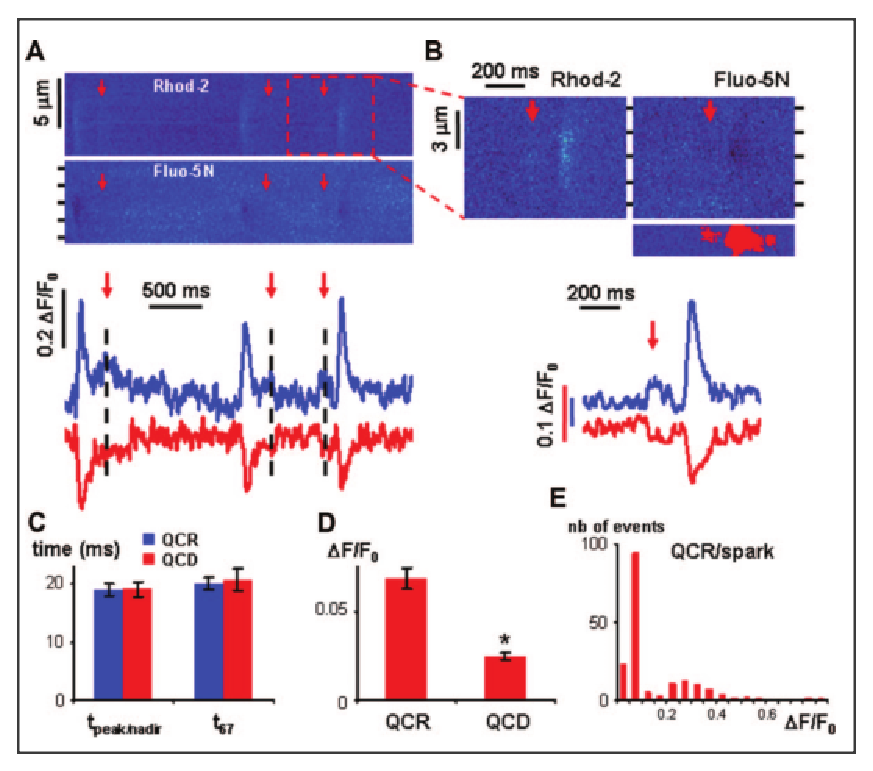
\includegraphics[height=6cm,
    angle=0]{./images/quark_brochet11.eps}}
  \caption{$\Ca$ quarks}
\label{fig:quark_brochet11}
\end{figure}


\subsection{$\Ca$ blinks}
\label{sec:calcium_blink}

Mirror the local increase subspace calcium is a local depletion of calcium in
the nanometer-sized $\Ca$ stores - the junctional cisternae of the SR and wider
SR. This lumenal $\Ca$ decreases is called $\Ca$ blinks \citep{brochet2005}.
The indicator Fluo-5N was loaded into the SR to measure this change in SR
calcium \citep{kabbara2001}. However, the change in the connected free network
SR is below detection ability\citep{brochet2011}. A possible explanation for
this is the diffusion limited caused by microanatomy structure. This concept
has been incorporated in spark model to emulate a mechanism of spark termination,
yet has not been observed experimentally at that time. \citep{brochet2011} has
reported it recently in rabbit ventricular cells.

\begin{framed}
\citep{brochet2011} used 5$\muM$ Rhod-2 AM to measure cytosolic $\Ca$. To study
$\Ca$ sparks and $\Ca$ waves, they block NCX (i.e. extracellular Na is replaced
by equimolar $\Li$). Electrical stimulation was 0.5Hz.  Using Fluo5N
(Sect.\ref{sec:fluo5N}), we can measure lumenal $\Ca$ dynamics. 

Line-scan image was generated with sampling rate 0.75-1.5ms per line and 50nm
per pixel (i.e. $0.05\mum$ per pixel).  
\end{framed}

\begin{figure}[hbt]
  \centerline{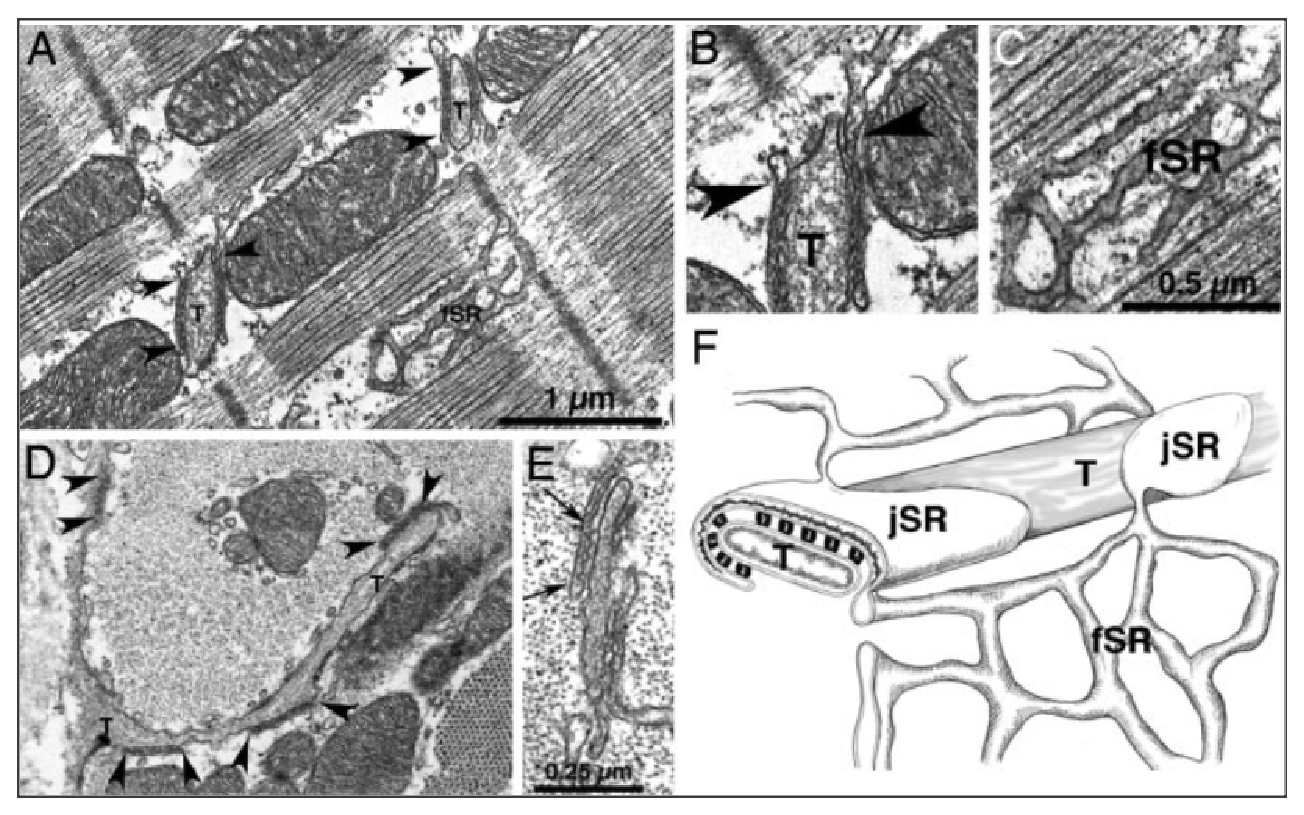
\includegraphics[height=5cm,
    angle=0]{./images/rabbit_SR_anatomy.eps}}
  \caption{SR anatomy of rabbit cardiac cells\citep{brochet2011}}
\label{fig:SRanatomy_brochet11}
\end{figure}

$\Ca$ sparks is wider and can spread to adjacent JSR,
Fig.\ref{fig:spark_blink_brochet11}. Compared to spark, blink is much more
confined, with FWHM of 0.8$\mum$.
\citep{brochet2011} measured FWHM of $1.01\pm 0.05\mum$. The nadir of the store
depletion is after the peak of the spark 10ms. The rate of refilling is 35
s$^{-1}$ (i.e. 6-fold faster than recovery of local $\Ca$ release after a
spark). To compare the change over time, the spark-blink pairs were plotted
together. The fitted data shown:
\begin{enumerate}
  \item Blinks: $\Delta F/F_0 = -0.06$, $\tau_\text{nadir} = 21ms$, and
$\tau_\text{recovery} = 33$ (ms), FWHM = 0.8$\mum$. The improved measurement
shown $\Delta F/F_0 = -0.013$,  $\tau_\text{nadir} = 32ms$ (i.e. trail the peak
of spark by 11ms, and slightly bigger FWHM = 1.0$\mum$.
\item Sparks: $\Delta F/F_0 = -0.30$, $\tau_\text{peak} = 21ms$, and
$\tau_\text{recovery} = 43$ (ms), FWHM = 2.2$\mum$.
\end{enumerate}

The magnitude of JSR depletion is about 85\% while that in the NSR is about 30-35\%.
This gradient explains a diffusion restriction connecting NSR and JSR
\citep{cheng2008cs}. In other studies, a local decrease in SR $[\Ca]$ is about
40\% \citep{brochet2005, zima2008tcas}. 

\begin{figure}[hbt]
  \centerline{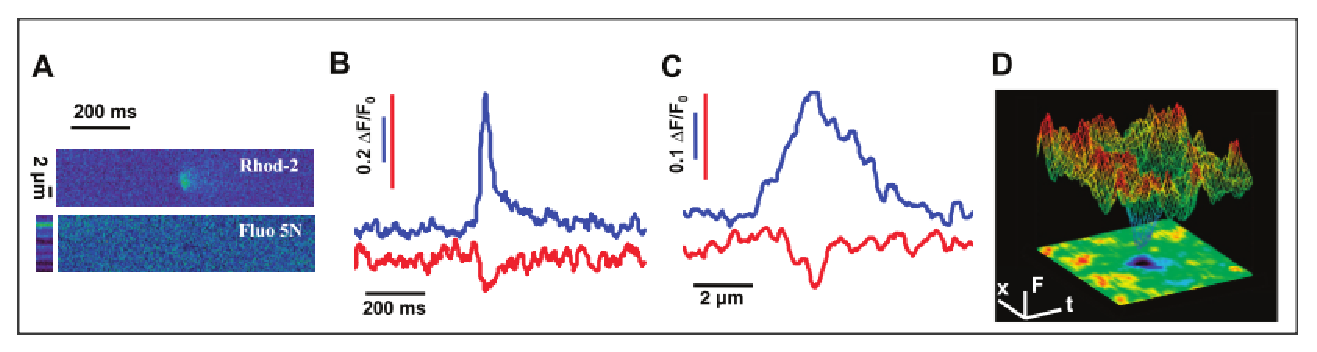
\includegraphics[height=3cm,
    angle=0]{./images/ca_blink_cheng08.eps}}
  \caption{$\Ca$ blinks mirrors $\Ca$ spark (intact rabbit ventricular
  myocyte with fluorescence fluo 5N and rhod2 in SR lumen and myoplasm,
  respectivey): (A) line-scan image is generated using F/F0), (B) time courses,
  (C) spatial profiles }
\label{fig:ca_blink_cheng08}
\end{figure}


\begin{figure}[hbt]
  \centerline{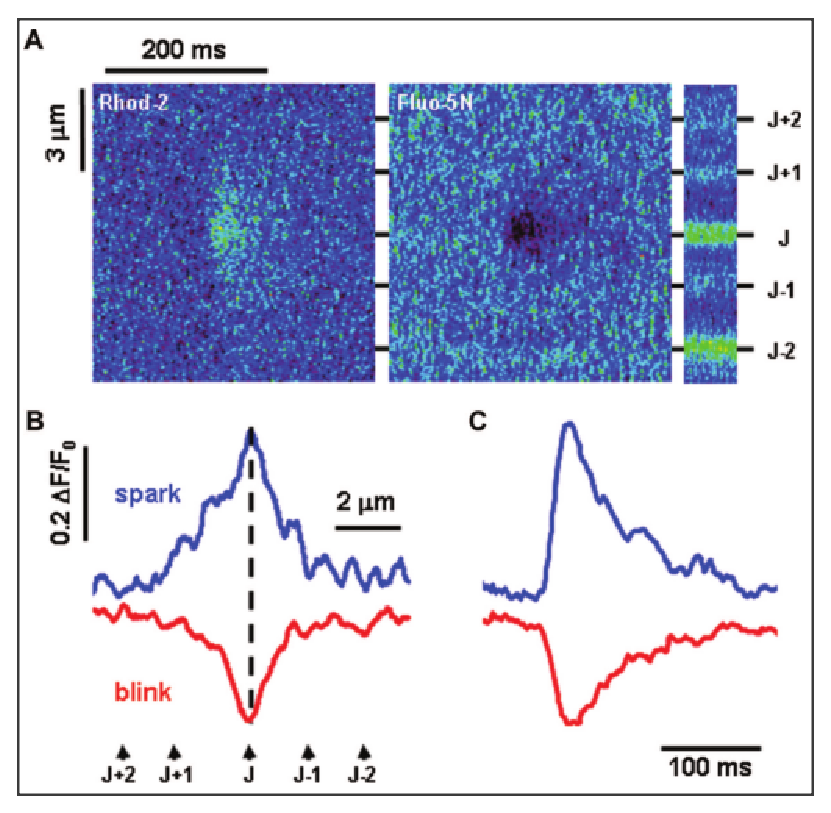
\includegraphics[height=3cm,
    angle=0]{./images/spark_blink_brochet11.eps}}
  \caption{FWHM = $1.01\pm 0.05\mum$ (blink aligned well with the JSR (J-th)).
  The $\Ca$ spark span wider, to adjacent JSR (J-1, J+1) with FWHM $2.27\pm
  0.12\mum$}
\label{fig:spark_blink_brochet11}
\end{figure}

The receovery time of spark-blink can vary widely, depending on the
cut-off. For example, spark decay ranges from 25ms (5\% cut off) to 95ms (95\%
cut-off). This can be due to blurring artifact from confocal imaging. A more
careful investigation from \citep{brochet2011}, they showed that
$t_\nadir=29.6\pm 1.4$ (ms), and $t_{67}=55.5\pm 2.6$ (ms).

\subsection{$\Ca$ embers}

$\Ca$ embers was first described as faint tail of voltage-elicited frog sparks
\citep{gonzalez2000}. Later on, $\Ca$ embers were recorded from rat skeletal
muscle under very artificial conditions \citep{zhou2003}.  For embers, FWHM was
$\sim 2\mum$ in rat and $\sim 1.5\mum$ in frog. Amplitudes are 33\% smaller and
rise times was 50\% longer in the rat. It means that the difference is
significant.


\subsection{$\Ca$ sparks with IP3}

A direct application of 10$\muM$ of IP3 produced a transient of 21\% increase in
the frequency of $\Ca$ sparks, yet accompanied by a 13\% decrease in spark
amplitude and a decrease in 7\% of SR $\Ca$ load in rabbit ventricular myocytes.
This change was inhibited by applying IP3R-antagonist: 20$\muM$ 2-APB and
heparin (0.5mg/ml) \citep{domeier2008}.


\subsection{$\Ca$ sparks in skeletal cells}
\label{sec:calcium-spark-skeletal-cell}

In skeletal cells, $\Ca$ sparks occur at the triadic junctions
(Sect.\ref{sec:triad}), not the dyadic junction as in cardiac myocytes. Before
the discovery of sparks, the movement of calcium from the release sites to the
sarcomere for frog skeletal muscle was first modeled by \citep{cannell1984}. In
skeletal muscle, the most important calcium-binding proteins are troponin (Tpn),
parvalbumin, and calsequestrin (CSQ). The binding of troponin (which reside on
the thin filaments), leads to tension production. Parvalbumin is the soluble
protein found with high concentration in the myoplasm of some muscles.
Calsequestrin is the low-affinity high-capacity calcium-binding proteins, that
serves as the main calcium buffer, localized at the junctional SR (terminal
cisternae) to allows large amount of calcium to be stored here without an
excessively high free calcium.


\section{Model a CaRU}
\label{sec:model-caru-1}

Each CaRU is modeled with two restricted compartments: the dyadic
subspace and junctional SR, as shown in Fig.~\ref{fig:CaRU}.
What we're interested is the movement of $\Ca$, i.e. the change in $[\Ca]$;
calcium fluxes are denoted by $J$. As the fluxes are defined as concentration
change per sec, all fluxes need to be defined based on a given volume. For
easily maintenance, all fluxes are defined over $V_\myo^T$.
\begin{figure}[hbt]
  \centerline{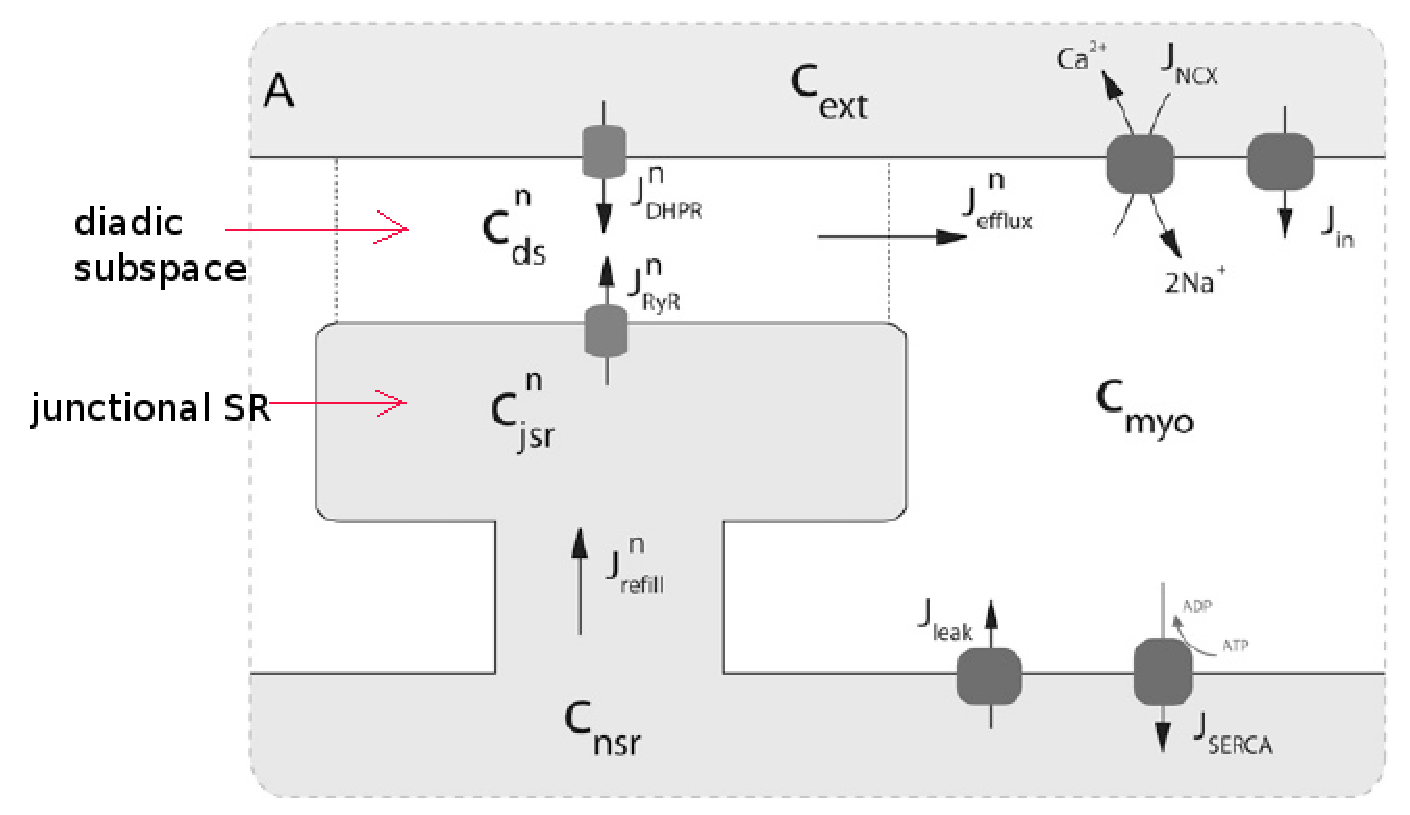
\includegraphics[height=6cm]{./images/CaRU.eps}}
  \caption{A diagram for a CaRU}
  \label{fig:CaRU}
\end{figure}


We will see all this in Chapter~\ref{chap:ap_ventricular_myocyte_localcontrol}.
Suppose that there are totally $N$ CRUsin a cardiac cell and $n$ is
used to index an individual CaRU.
\begin{itemize}

\item $J_{in}$: the background $\Ca$ flux.

\item $J^n_{DHPR}$: the $\Ca$ flux through the L-type DHPR
  (dihydropiridine receptor) channels at $n$-th CaRU.

\item $J_{NCX}$: the  $\Ca$ flux through \ce{Na+}/$\Ca$
  exchanger.

\item $J^n_{RyR}$: the  $\Ca$ flux through RyRs channels in the
  $n$-th CaRU

\item $J^n_{refill}$: the $\Ca$ flux from network SR (NSR) to the
  junctional SR (JSR) in the $n$-th CaRU.

\item $J_{leak}$: the $\Ca$ passive leak from NSR to myoplasma
  through leak

\item $J_{SERCA}$: the $\Ca$ flux from NSR to myoplasma through
  SR  $\Ca$-ATPase (SERCA) pumps.

\item $J_{efflux}$:  the $\Ca$ flux from a single dyadic subspace
  to the myoplasma.
\end{itemize}
The number of RyRs and LCCs in each CRU was mentioned in
Sect.\ref{sec:CRU_size}. 

As the change in [$\Ca$] is the central factor, the dynamics of
[$\Ca$] in different local area is examined. This process
requires knowing the concentration of $\Ca$, denoted by $c$, at
different local regions.

\begin{itemize}
\item $c^n_{ds}$ or $[\Ca]_\ds^\ii$: the [$\Ca$] in the dyadic subspace of the
  $n$-the CaRU

\item $c^n_{jsr}$ or $[\Ca]_\jsr^\ii$: the [$\Ca$] in the JSR of
  the $n$-the CaRU

\item $c_{nsr}$ or $[\Ca]_\nsr$: the [$\Ca$] in the NSR

\item $c_{myo}$ or $[\Ca]_\myo$: the [$\Ca$] in the myoplasma

\item $c_{ext}$ or $[\Ca]_o$: the extracellular [$\Ca$]
\end{itemize}
Calcium ions that escape from the dyadic subspace are unlikely to return due to
rapid dissipation into the larger surrounding cytosolic space.

When a single LCC open, $[\Ca]$ is estimated to be elevated above 10mM within
760nm of the channel mouth, Fig.\ref{fig:CRU_Sobie2006}(A). Also, the gradient
of $[\Ca]$ centered around the mount of the channel exists within the subspace.
This elavation is thought to be sufficient to activate RyRs in the jSR and
trigger a locally regenerative $\Ca$ spark from the cluster.

\begin{figure}[hbt]
  \centerline{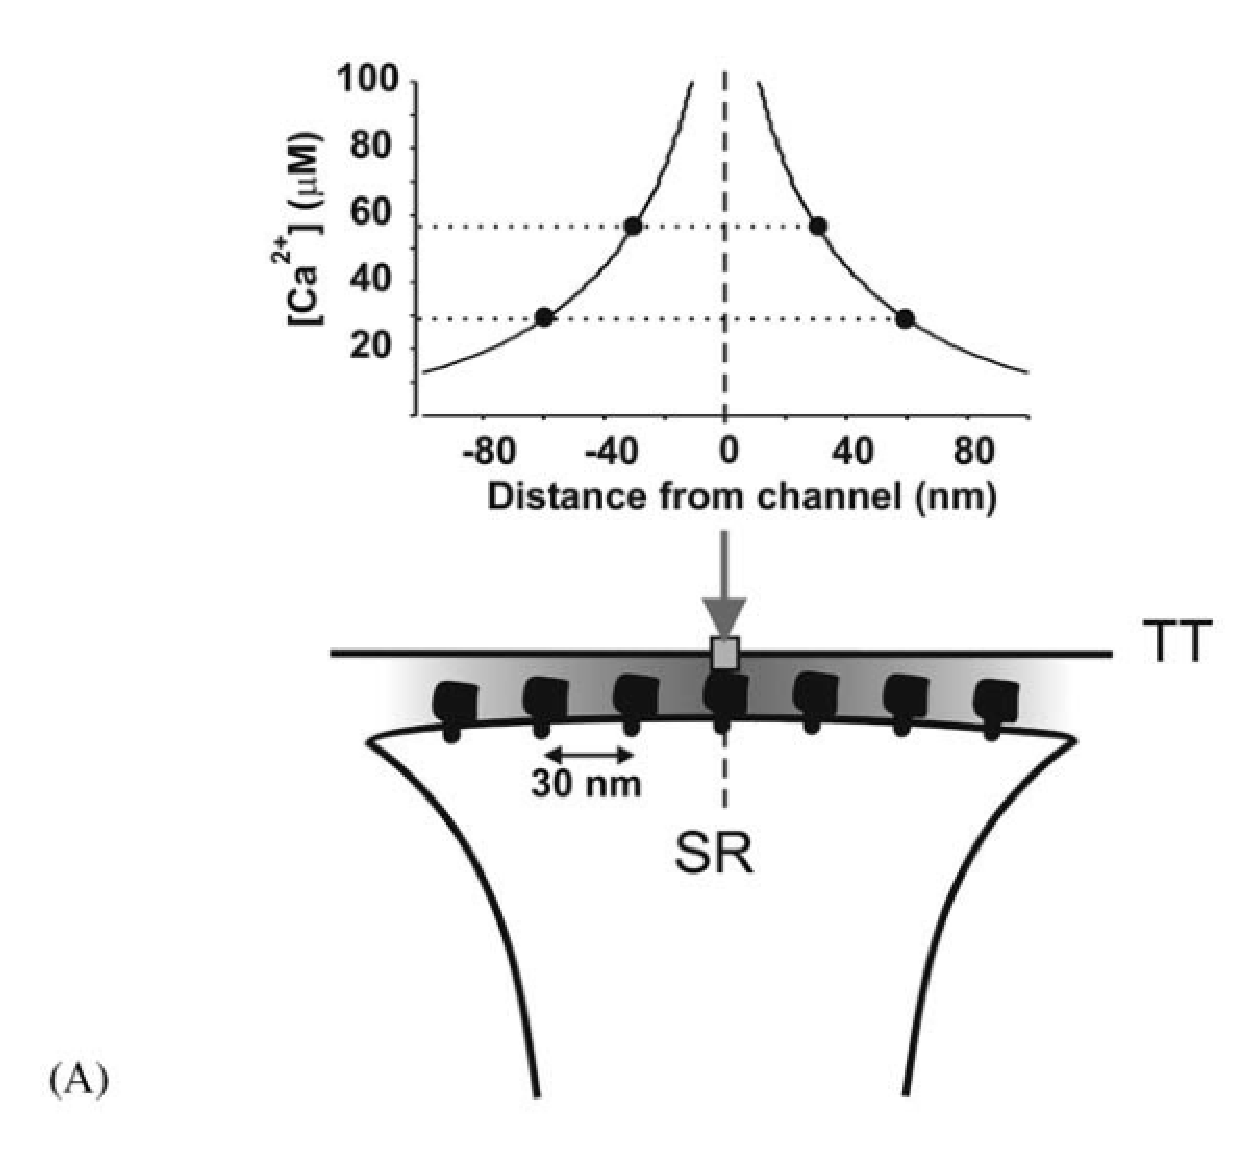
\includegraphics[height=5cm,
    angle=0]{./images/LCC_Sobie2006.eps},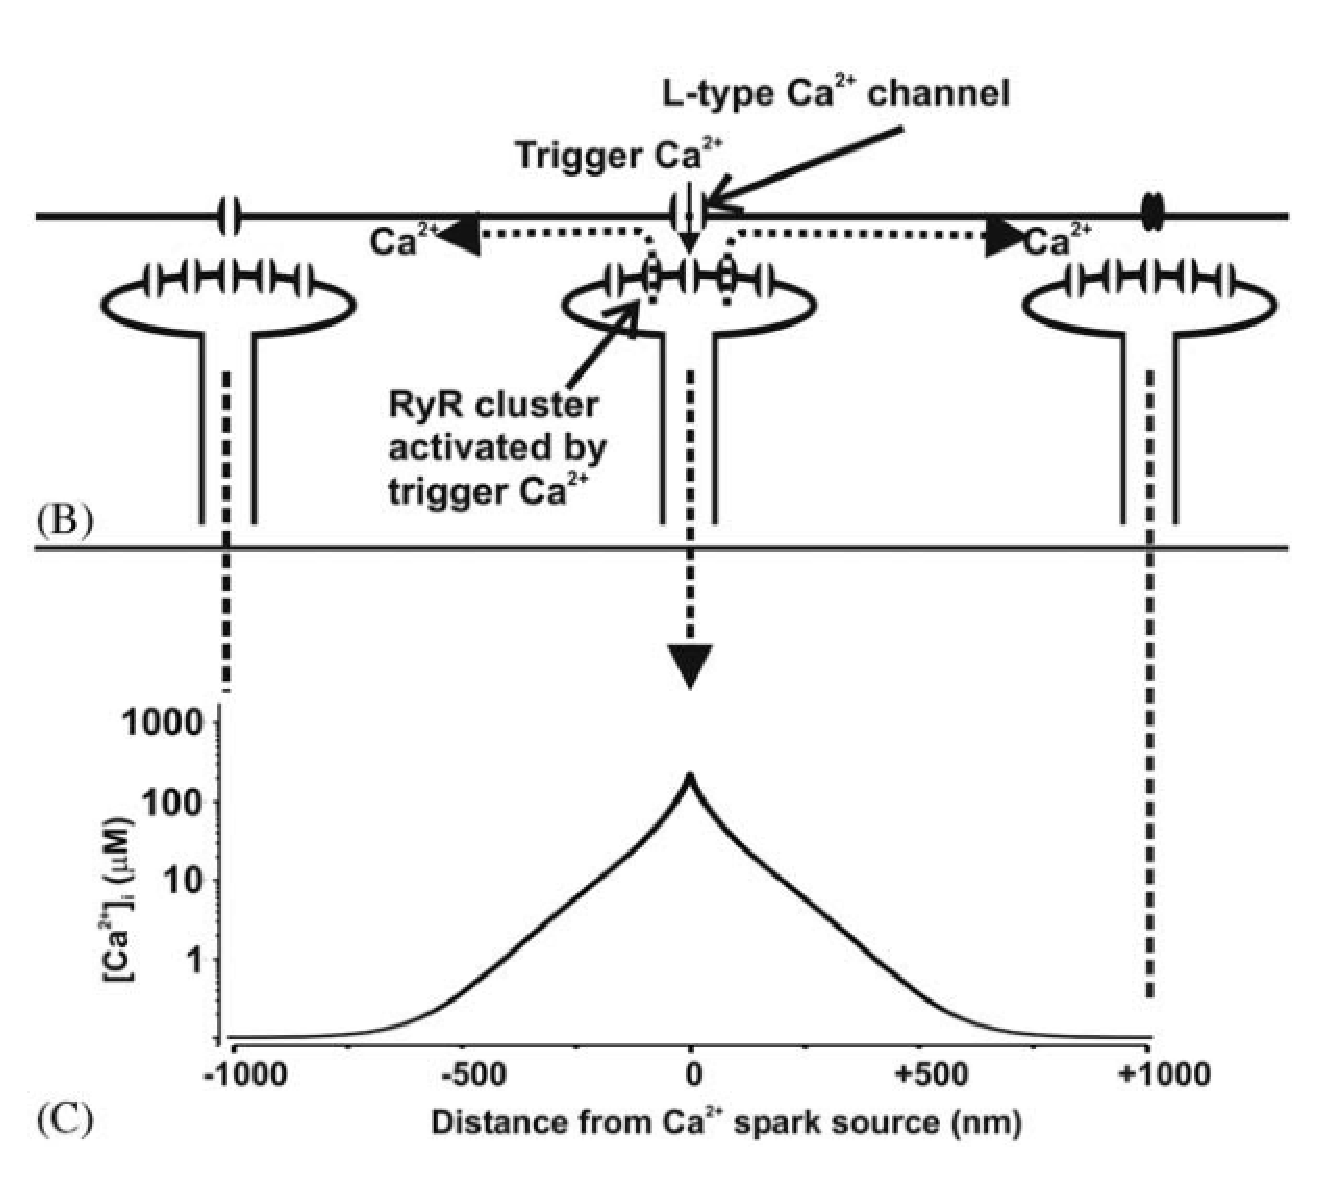
\includegraphics[height=5cm,
    angle=0]{./images/CRU_Sobie2006.eps}}
  \caption{Nano-scale and micro-scale of $\Ca$ level in heart cells
  \citep{sobie2006}: (A) a single LCC 0.5pA open for 0.5ms can trigger RyR
  located within $\pm 60$nm. (B) $\Ca$ signalling between release sites where
  $\Ca$ release from one site does not usually trigger release from neighboring
  sites. (C) $[\Ca]$ in the region surrounding the CRU using the published
  model \citep{sobie2002tcas}. At the end $\pm 500$ nm from the source, $[\Ca]$
  is elevated to 352nM at the end of an assumed of 10ms period release}
  \label{fig:CRU_Sobie2006}
\end{figure}


The release flux is either modelled as
\begin{enumerate}
  \item A single point source, as a delta function $J_\ryr\delta(r)$.
  \item A cluster of RyR, where the channels gate stochastically
  (Sect.\ref{sec:spatial-model-single}).
\end{enumerate}
 
The diffusion of calcium from the release site to the bulk can be modelled
as
\begin{enumerate}
  \item Fickian diffusion
  \item anomalous (or non-Fickian diffusion) 
  \begin{equation}
  \frac{\partial c(r,t)}{\partial t} = D_\alpha
  \frac{1}{r^2}\frac{\partial}{\partial r} \left( r^2
  \frac{\partial^{1-\lambda}}{\partial t} \frac{\partial^\beta c(r,t)}{\partial
  r^\beta} \right) + f(r,t)
  \end{equation}
  with $c(r,t)$ is calcium concentration at a distance $r$, at time $t$ to the
  release site; $D_\alpha$ is anomalous diffusion constant, $f$ is reaction
  function (representing sources or sinks). $0 < \lambda \le 1; 0 < \beta < 2$;
  when $\lambda=\beta=1$, the equation becomes Fick's law. 
  
  The range of $\beta$, $0 < \beta < 1$ or $1<\beta<2$ correspond
  to long or short jump of the random walker, respectively (or aka
  superdiffusion or subdiffusion). The spark data are
  best depicted with $\lambda=\beta = 1.25$, suggesting a subdiffusion model in
  the milieu of cytoplasm. However, the physical basic for this non-Fickian
  behavior is unclear; yet it is thought to reflect the complex microscopic and
  nanoscopic structures and viscoelastic properties of the cytoplasm. 
  
  
\end{enumerate}
 
Based on \citep{franzini_armstrong1998, franzini_armstrong1999ssd},
SR-TT contains nearly crystalline arrays of RyRs organized in
clusters. RyRs are organized in hemotetrameric units, each touching
four neighbors via a small protein, known as FK506-binding protein, at
or near the point of contact~\citep{Sharma1998, wagenknecht1997}.


\subsection[LCC influx]{LCC influx ($I_{dhpr}$)}
\label{sec:lcc-influx}

LCC - aka dihydropyridine (DHPR) - is the major type of Ca channel in
ventricular myocyte that is mediated (activated and inactivated) by voltage and
$\Ca$~\citep{lee1985icc, shirokov1993cdi}. LCC influx is the major influx
pathway of $\Ca$ across sarcolemma during each heartbeat. However, this influx
is much smaller than $\Ca$ release from SR (Sect.\ref{sec:sr-release}).  

\textcolor{blue}{The models of DHPR is discussed in
  Chap. \ref{chap:dhpr-models}}.
Even though the activation of LCC is voltage-dependent and is usually simple,
the inactivation is more complex. In the early models, the $\Ca$-induced
inactivation of LCC is thought to be a function of the bulk myoplasm, denoted by
$[\ce{Ca^2+}]_{myo}$ or $[\ce{Ca^2+}]_i$ \citep{difrancesco1985mcea,
luo1994dmc_a, nordin1993cmm}. However, $[\ce{Ca^2+}]_{ds}$ - the calcium
concentration in the diadic subspace between LCC and RyRs is generally thought
to have different dynamics than $[\ce{Ca^2+}]_{myo}$. Thus, later models suggest
that gating of LCC is the function of a local concentration of Ca in this
microdomain, known as $[\Ca]_\ds$~\citep{imredy1992scd, shannon2000pfs}. This is
consistent with the spatially and temporally localized SR $\Ca$ release events,
known as {\bf $\Ca$ sparks} which is considered as the elementary events in
cardiac cells (Sect.~\ref{sec:ceca2+-sparks}).

If the LCC is modelled in a mode-switching formula, i.e. Markov LCC
model, one way to explain the above hypothesis is that the SR release
induces the channel to the mode in which openings has a very low
probability, i.e. effectively inactivating the
channel~\citep{imredy1994mcs}. The exiting from this mode is thought to
slow down while the cell is depolarized. The effective inactivation of
the channels persists in short (20ms) compared to the much longer AP
(200ms). Many models use this mode-switching formula, e.g. in diad
models~\citep{rice1999mgg, stern1999lcm}, and in integrated cell
models~\citep{jafri1998cad, rice1999mst,winslow1999,greenstein2002}.


\subsection[SR $\Ca$ release]{SR $\Ca$ release ($I_{ryr}$)}
\label{sec:sr-release}

There are three types of RyRs: RyR type-1, cardiac RyR2, and RyR3
(read Chap.~\ref{chap:ryr-models}). In cardiac, we only focus on RyR2.
The opening of RyR is a non-linear relation to the SR $\Ca$ load
- or luminal $\Ca$. Experiments show
that~\citep{bassani1995fsr,shannon2000pfs}
\begin{itemize}
\item at low SR content (lumenal $[\ce{Ca^2+}] < 500\mu$M): $\Ca$
  release is quite small

\item at high SR content (lumenal $[\ce{Ca^2+}] > 500\mu$M):
  $\Ca$ release increase steeply
\end{itemize}
The reason is that at high luminal concentration, $\Ca$ bind to
CSQN and help CSQN forms dimers (when $[\ce{Ca^2+}]$ luminal reaches
$500\mu$M) or higher order polymers (...reaches a few millimolar).
Polymerized CSQN help reduce the $\Ca$ spark refractory periods

\begin{framed}
  Refractory periods is the time required for the excitable membrane
  to be ready for the next stimulus after returning to the resting
  stage, i.e. during that time, the stimulus cannot trigger any event.
\end{framed}

\begin{framed}
  CSQN is the primarily buffering protein, i.e. $\Ca$ holding
  protein, localized in the JSR~\citep{franzini_armstrong1987sct}. The
  regulation of luminal $\Ca$ to the sensitivity of RyRs is via
  the interaction of $\Ca$ luminal buffer CSQN with the two small
  SR proteins triadin-1 and junctin (T/J).
\end{framed}

Indeed, the behavior of SR release is quite complicated. For a fixed
trigger influx, 
\begin{itemize}
\item if the trigger influx is below a threshold, essentially little
  or no SR release occurs~\citep{bassani1995fsr, shannon2000pfs}
\item if the trigger influx is above this threshold, 
  \begin{itemize}
  \item SR release is a steeply increasing function of SR
    load~\citep{bassani1995fsr, shannon2000pfs},
  \item some found it is a linear change~\citep{janczewski1995esr}.
  \item some found it is a nonlinear function of both the gain of SR
    release (i.e. the integral of SR release flux divided by the
    integral of LCC influx) and the release fraction (i.e. the
    integral of SR release flux divided by the total [Ca] in the SR,
    including that bound to buffers)\citep{shannon2000pfs}.
    \begin{itemize}
    \item if the SR uptake is blocked, the release fraction is about
      10-60\%~\citep{bassani1995fsr}
    \item in normal condition, the release fraction is about 80\%
      \citep{trafford1999nrr}; and can be more than 100\%, suggesting
      that Ca uptake during the release process may be released again.
    \end{itemize}
  \end{itemize}
\end{itemize} 

There are different ways to model the SR release 
\begin{enumerate}
\item as a mechanism in which RyR open probability increase with SR load,
  some other factors like a positive feedback of Ca via RyR release
\item as load dependence with a representation of SR control in which
  {\bf calsequestrin} (a JSR-specific protein inside SR) is assumed to
  interact with RyR to modulate RyRs' open
  probability~\citep{ikemoto1989prc, snyder2000mmc}
\begin{verbatim} 
    prob.open  = f(Ca load, active of calsequestrin)
\end{verbatim}
  e.g. in skeletal muscle\citep{gilchrist1992icd}. Also, it assumes Ca
  binding to the cytoplasmic side of RyR can also feedback on
  calsequestrin ability to liberate RyR, i.e. active of calsequestrin
  = f(Ca binding to RyR on cytoplasmic side). Though, this assumptions
  lack experimental evidence to support, its possibility does exist
  for such complex interaction.
\end{enumerate}

The unitary RyR current, depending on conditions, vary from 0.4 to 4
pA. The number of RyR open in a single spark shown a U-shape
dependence on the unitary RyR current. 

Efforts to add CSQ into the jSR includes, but not limited to:
\citep{snyder2000mmc} (Sect.\ref{sec:snyder_2000}).

\section{Spark characteristics}
\label{sec:spark-characteristics}

A $\Ca$ spark is often characterized based on $\Delta [\Ca]$ or $\Delta F/F0$,
the full duration, full duration at half-maximal amplitude (FDHM), the full
width, the full width at half-maximal amplitude (FWHM), the rise time (time to
peak) and the half time decay $\tau$ (fitted by a single exponential function),
and maximum steepness of upstroke ($(\Delta F/F0)/$sec). The rise time is the
time (in msec) of $\Ca$ release from the SR until full peak is achieved. $\Ca$
signal mass (both the amplitude and width) correlate with the amount $\Ca$ released.
So, it's hypothesized that calcium diffusion (isotropic or anisotropic?? and the
diffusion constants), the dye diffusion constant (that may determine the spread
of the spark). $\Delta F=F-F0$ where F0 is the background value calculated by
taking the average of CaF at a few time points before the activation of sparks;
and F is the dynamics fluorescence value of CaF.

$\Ca$ sparks are highly localized both in time (duration $\sim$ 30 ms) and in
space (FWHM $\sim 2\mum$) \citep{cheng1996ecc}. The site at which this local
elevation occurs is called calcium release unit (CRU)
(Sect.\ref{sec:cru_calcium_release_unit}).
These sites are suggested to space regularly at 1.8$\mum$ intervals
corresponding to T-tubules at Z-lines \citep{shacklock1995}.
After the spark is triggered at a particular CRU, the probability for next spark
to occur at that CRU is immediately decreased and this probability slowly
recover after $\sim 400$ms.
Different hypothesis were given to explain for this
\begin{enumerate}
  \item The recovery of junctional SR  (jSR) is slow ($\sim 200$ ms) which is
  controlled by the $v_\rf$ rate from nSR to jSR.
  \item RyR channels is adapted, i.e. adaptation approach, which is modeled with
  adaptation for RyR channel.
\end{enumerate}

\citep{cheng1993cse} observed spontaneous spark in quiescent rat ventricular
myocyte. \citep{lopez-lopez1994} observed evoked spark in canine during membrane
depolarization and they hypothesized that the variable gain can be due to
$I_\Ca$ affect amount of $\Ca$ release (this is incorrect).
\citep{cannell1995b} pointed out that the gradeness of $\Ca$ release can be
adjusted by altering  the probability of spark generation, not by altering the
spark duration as it was wrongly suggested by \citep{lopez-lopez1994}. The {\bf
variable gain} is the term refering to the different gains using different
$V_\stim$, i.e. $V_\stim$ affect $I_\Ca$ which then affect spark triggering
probability and eventually affect total $\Ca$ transient.
\citep{lopez-lopez1995} shown that the influx of $\Ca$ through LCC is
more efficacious than through NCX. \citep{lopez-lopez1995, cannell1995b}
shown that the local transient is independent of voltage, as well as the
duration of the $I_\Ca$.

\subsection{Criteria to be a spark}

Using fluorescence signal, the criteria to be a spark is based on the
normalized fluorescence signal, i.e. F/F0, local peak. If the local peak
elevations exceed 1.5 times the background level, or $F/F0\ge 1.5$ or $\Delta
F/F0 \ge 0.5$, then it's a spark \citep{howlett2006}. 

There are softwares to detect sparks automatically and do other analysis too
\citep{picht2007}.

\subsection{Spark duration}

Experimental data from studies of \citep{cleeman1998,niggli1999} shown
that spark duration  is relatively constant (10-30ms) and is independent from both SR
$\Ca$ load and distolic calcium level.
$\Ca$ release during  the spark is determined by the intrinsic gating of the SR
$\Ca$ release channel  (i.e. the mean open time and the possible states under
hyperphosphorylation condition). 

\subsection{Spark peak}

Spark peak is $\approx 100$-fold increase compared to basal
level\citep{santana1996}. Definitely, it should depens on the number of channels
involved. So far, there is no significant difference between spontaneous
sparks (which require no influx $\Ca$) and evoked sparks (trigger by influx of
$\Ca$ via LCC, but not NCX). A typical $\Ca$ spark has a rapid rise ($\sim$10
ms, time to peak), and a moderately quick decay kinetics ($\sim$ 20ms, half-time
decay). The spark is confined within a sphere of diameter 2$\mum$ or $\sim$ 8 fl
by volume.

There are obstacles in evaluating spark amplitude. The sparks are recorded by
imaging using line-scanning technique. The reported amplitude depends as much on
the true amplitude of the height of the fluorescent object. Using computational
models, \citep{pratusevich1996} (Sect.\ref{sec:prat-balke-1996}) suggested a
single mode (i.e. monotonic spark amplitude distribution) for calcium spark
amplitude, based on the historogram of spark amplitude. It as then confirmed
experimentally in cardiac and skeletal muscle by \citep{cheng1999}. However,
\citep{bridge1999} found it to have a mode.

The spark amplitude is about 100 nM. At quiescent condition, the spontaneous
spark rate is low ($\sim$ 100 spark/cell/sec) \citep{cheng1993cse}. During AP,
it showed an increase of about $2.2\times 10^4$-fold, i.e. from 1 s$^{-1}$ to
144 s$^{-1}.\mum^{-1}$ in a linescan encompasing 150$\mum$
\citep{cannell1994snu}. If the opening rate is proportional to the square of the
local $[\Ca]$ concentration, then this increase in rate require the local
concentration to increase by a factor of about 150, i.e. it reaches 15$\muM$
from resting value 100nM. This local domain is termed ``fuzzy space'' by
\citep{niggli1990,lederer1990}.

It has been observed that synchronized sparks along the transverse direction
which may be the clue of peripheral RyR cluster surrounding a normal CRU
\citep{parker1996csi}.

\begin{enumerate}
  \item \citep{cheng1993cse} estimated peak $\sim 0.3\muM$ in 10ms.
  However, this value is not accurate due to the limited kinetics . 
  \item \citep{smith1998} estimated it $> 10\muM$ (averaged by microscope
  blurring in a 0.5$\mum$ region)
  \item ~\citep{collier1999}
estimated the $\Ca$ spark amplitude in rat ventricular myocytes is
$289\pm 3$nM (n=345), decay half-time is about $20.8\pm0.2$ms, and
FWHM is $1.4\pm 0.03\mum$.
\item \citep{brochet2011}, in rabbit ventricular myocytes, estimated FWHM as
$2.27\pm 0.12\mum$. (a volume of 10x greater than a blink). 
\end{enumerate}

In terms of using fluorescence, the $\Ca$ sparks double the resting $\Ca$-bound
fluorescence at the peak, i.e. $F/F0=2.0$ or $\Delta F/F0 = 1.0$. The spark
occupies a tiny region ($\sim 2\mum$ in diameter) \citep{cannell1999}. 


\subsection{Blink nadir}

Blink is the mirror depletion of $[\Ca]_\jsr$ during a spark. It's now widely
accepted that dynamic changes in $[\Ca]_\jsr$ play important regulatory roles.
The development of Fluo-5N as an indicator for SR $\Ca$ has enabled this study
\citep{Sobie2012}.

Simulation of jSR depletion requires certain assumptions about jSR volume, jSR
buffer concentration, RyR cluster size, $\Ca$ flux via single RyR, and the rate
of jSR refilling. Even though Fluo-5N is available to record SR $\Ca$, the
converting from fluorescence signal to free $\Ca$ is not straightforward.
\citep{Sobie2012} estimated that about 50,000 $\Ca$ ions are present in each jSR
before $\Ca$ release. Using single RyR current of 0.5pA, which maps to a flux of
1500 $\Ca$ ions per ms. So, with 8 opening RyR can deplete jSR $\Ca$ completely
in less than 4ms. It means that the current becomes smaller during the release
which make the flux is no longer a constant. During the release, jSR is also
refilled from the neighboring nSR as well. 

Computational models predicted strong depletion with roughly 90\%
\citep{sobie2002tcas, Ramay2010}.  Experimental data only show about 50\%
depletion \citep{brochet2005, Terentyev2008}. We're not sure which one is better
as blinks may underestimate the extent of jSR depletion


\subsection{Po (open probability of RyR2)}


Peak of $P_o$ of RyR2 was estimated about 0.76 during normal AP
\citep{jafri1998cad}. Fractional SR calcium released was estimated about 35\%
total SR calcium \citep{bassani1995fsr} using $[\Ca]_o=2$mM in ferret
ventricular myocytes. A lower $[\Ca]_o$ will yield a lower fractional of SR
$\Ca$ released. 

RyR open probability ($P_o$) was 0.001 at 10$\muM$ and increased to a maximum of
$\approx 0.5$ at 100$\muM$ and remained at this level for
about 15ms before RyR started to close \citep{laver2012}
(Sect.\ref{sec:laver_cannell_2012}).

\subsection{Spark width}

FWHM is about 2$\mum$ which is a challenging problem is modelling as no spark
model can reproduce this character of sparks. Spark sites are seperated by
$1.8\mum$ in longitudinal in resting cardiac cell. The distance is closer in
transversal direction, and more variable \citep{parker1996csi}.


\subsection{Spark frequency}

The spark frequencey can be defined in different ways: 
\begin{enumerate}
  \item number of sparks per whole-cell per sec (sparks/cell/sec)
  \item number of sparks per line-scan per sec (sparks/(100$\mum$.sec))
  \item number of sparks per volume per sec (sparks/(1$\mum^3$.sec))
\end{enumerate}

\citep{cheng1993cse} estimated spark frequency in a line-scan images as 1.6
spark/line-scane/sec (survey 70-100 sarcomeres), which can increases up to
3.53$\pm 0.75$ sparks/line-scan/sec after 1-3min upon exposuring to 100-300nM of
ryanodine. The normal spark frequency suggests a spark rate of about 100
sparks/cell/sec at rest. Whole-cell stretch (sarcomere length increase about
8\%, i.e. from 1.87$\pm 0.032\mum$ to 2.027$\pm 0.035\mum$) increase the
ventricular myocyte spark rate to 130$\pm$ 6.4\% after 5sec \citep{iribe2009}.
Spark rate increases only at the stretched region.

\citep{howlett2006} compared between normal (2.12$\pm 0.96$
sparks/(100$\mum$.sec)) vs. aged mice (5.59$\pm 1.29$ sparks/(100$\mum$.sec))
(assessed at physiological temperature $37^\circ$C) and saw an increase in
spontaneous spark rate. A similar studies conducted at room temperature gave the
similar result too \citep{zhu2005}. There are different possible reasons to
cause this increase in spark rate. However, it wasn't caused by an increase in
SR $\Ca$ load in aging heart, or increase in cytosolic calcium, or a change in
resting potential. Other possible but untested features: ATP, $\H$, calmodulin,
cADP ribose, and protein phosphatases that influce gating of RyR2s.
Spark amplitudes don't change, so the number of RyR2 per spark is the similar
between young adult and aged cells. However, spark duration is longer in aged
cell. It's suggested that RyR coupling is modified in aged cells. In essence,
this lead to significant age-related change in $\Ca$ transient at whole-cell
level too (smaller in aged cells).


\subsection{Spark: symmetric vs. asymmetric}

In cardiac cells, sparks are often asymmetric, being larger along x-axis than in
the transverse (y- and presumably z-axis) \citep{parker1996csi}. 

Important sparks characteristics includes:
\begin{enumerate}
  \item spark rise time (time to peak): $\tilde 8$ms
  \item amplitude: $\Delta F/F0 \sim 1$
  \item spark duration: 20-30ms
  \item spark spread: FWHM $\sim 2\mum$
\end{enumerate}
The most challenging problem so far is to replicate spark spread {\it in
situ}. Computational models with realistic model parameters have been able to
produce spark with FWH of 1.0-1.5$\mum$ \citep{smith1998, sobie2002tcas}.
This discrepancy has been ascribed to a few probable reasons: (1) calcium sparks
can be the result of multiple CRUs rather than a single CRU (e.g. 2 dyads on
both sides of the T-tubules), (2) RyR in the NSR (rogue RyR) might contribute to
the spatial spread, (3) the size of the dyad might be larger than it is
currently thought \citep{soeller2004}. 

\citep{izu2001lcg} claimed that $I_\LCC$ may affect to the calcium spark spread,
where larger $I_\LCC$ current can generate larger spark spread. Yet the larger
current is an unrealistic assumption. 



\section{How to simulate calcium dynamics in a microdomain}
\label{sec:spatial-model-single}

The scale of a calcium microdomain is 100-1000nm (The size of the subspace is
100-400nm in diameter, and 15nm in height). At the upper end of the considered
scale, (1000nm)$^3$ = 1 fl volume, with $[\Ca]$ = 100nM at rest, contains as
little as 60 $\Ca$ ions on average. So, even the activation of a single channel
can contribute significantly change to the dynamics of local calcium. As a
result, it's important to have an (exact) stochastic simulation of calcium.
As in a microdomain (0.5$\mum^3$), only a few 7-8 $\Ca$ ions are present on
average (at resting $[\Ca]=0.1\muM$), a more realistic simulation should include
the stochastic of $\Ca$ dynamics (both gating of channels and
reaction-diffusion of ions itself). However, the computational demand is a major
challenge.

\begin{framed}
NOTE: With the small subspace volume, at rest, the concentration 100nM
corresponds to 1 $\Ca$ ion in the subspace. This raised the validation of using
concentration to describe $\Ca$ in the subspace, and using diffusion to model
calcium transport within the dyadic subspace. Many models still assume using
concentration to quantify calcium level.
\end{framed}

Early models that do not model channels explicitly and assumed a constant
resting $\Ca$, ignoring the intrinsic stochasticity due to buffering and
diffusion, are completely deterministic, partial-differential-equation based
models \citep{smith1988, jiang1999, uttenweiler2002}. 

\citep{bhalla2004} introduced a simplified model of calcium buffering to model a
neuronal synapse using a single first-order reaction equations. A more
complicated approach where both $\Ca$ buffering and diffusion are treated
stochastically using Fokker-Planck equation \citep{winslow2006} (a
deterministic PDE describing the evolution of the probability density function
of all molecules's spatial positions).
\citep{keller2008} used Brownian dynamics simulation to study $\Ca$-dependent
signalling activated by calmodulin in a neuronal synapse. Here, each particle
wass treated explicitly, giving the most detailed picture. However, to avoid the
computational demand, $\Ca$ dynamics is typically treated on
a mesoscopic level, i.e. the algorithm tracks the total number of ions and
buffer molecules rather than the 3D path of individual reactant.

Another way is to use a {\it mixed computational approach}, i.e.
deterministic approach for calcium dynamics (reaction-diffusion, and buffering)
and stochastic algorithm to simulate channel gatings for ion channels: LCCs,
RyRs \citep{stern1997, stern1999lcm, greenstein2002, hinch2004mag} and IP3R
\citep{rudiger2007, shuai2007kmip3r, shuai2008}. This fusion of deterministic
and stochastic in hybrid simulation need to use very
small time steps, i.e. ``quasi-infinitesimal'' time increments.

The hybrid approach is a potential choice in cardiac cell modelling. To
understand how RyR distribution affects to the triggering and termination of
sparks, spatial model of a single CaRU is necessary. To model spatially the
cleft space, 10nm mesh can be used, with diffusion in 2D or 3D, depending on how
detail of the model. However, to avoid the extensive computational demand, a
{\bf mean-field approach} has also been applied where the explicit location of
individual channels are ignored. \citep{deremigio2008crs} suggested that when
single-channel models assumed a slow $\Ca$ inactivation, the kinetics of sparks
and puffs are less sensitive to the ultrastructure of RyR cluster in the lipid
bilayer. So, a mean-field approach is an acceptable approach.

\begin{framed}
  Assumption in Monte Carlo simulation: the set of channels in a diad
  is treated as a single stochastic system whose state
  (``macrostate'') is defined by specifying the Markov chain state of
  each of the individual channel. State transitionof individual
  channels are considered to take place instantaneously so that
  macrostate transition correspond to exactly a single channel
  transition. 
\end{framed}

\subsection{Gillespi's algorithm - exact stochastic}

The Gillespi method is described in Sect.\ref{sec:gillespie}. 

\begin{framed}
Transitions between functional states of channel proteins are usually modeled as
a Markov process where each state corresponds to a set of functionally
equivalent protein conformations \citep{smith2002}. The transition rates between
these states can be measured experimentally using voltage-clamp protocol. 
\end{framed}

The state vector $x(t) = (x_1(t), x_2(t), \ldots, x_N(t))$ denotes the number of
each reactant $x_i$ (i=1\ldots N) at time $t$ (NOTE: $N$ is the number of
species).

\begin{framed}
$x_i$ represent the number of ``particles'' of species $i$-th. The species can
be free $\Ca$, unbound buffers, bound Ca-buffers, channels in a given state. 

If we consider only the channels, $N$ represent the number of channel state,
$x_i$ represents the number of channels  in state $i$-th. The transition from
one state $i$ to another $j$ is  represented by $k_{ij}$. 
\end{framed}

Each of the $M$ reactions $R_j$ (j=1\ldots $M$)	has a reaction propensity
\begin{equation}
a_j(x,t) = c_j \times h_j(x,t)
\end{equation}
with $c_j$ is a volume-adapted stochastic rate constant and $h_j(x,t)$
represents the number of possible molecular combinations available for reaction
$R_j$ at time $t$. 

\begin{framed}
In simulating $\Ca$ dynamics in the microdomains, we have mono- and bimolecular
reactions:
\begin{enumerate}
  \item mono-: channel gating from one state to another, diffusion events,
  channel conductance: permeation of $\Ca$ ions through the  channel pore
  
  \item bimolecular : association and dissociation of $\Ca$ binding to
  buffer molecules and $\Ca$ channels 
\end{enumerate}

The stochastic rate constant $c_j$ is calculated from the macroscopic reaction
rate constant, i.e. $c_j=k_j$ (mono-) and $c_j=k_j/V$ (bimolecular; with $V$ is
single-voxel volume). In the classic Gillespie's algorithm, a single reaction
volume $V$ is considered. To account for diffusion events, the volume of inerest
$V_o$ is decomposed into a set of $n_v$ sub-voxels of volume $V=V_o/n_v$. 

With multiple reaction volumes, the diffusion rate is introduced using a
stochastic diffusion rate constant (of a species $i$-th, regardless of which
sub-voxel it reside, to another sub-voxel $V_k$) $d_{ik} = \frac{D_i}{(\Delta
x)^2}$, i=1\ldots $N$, and $k=1\ldots n_v$. This is described in \citep{elf2003}
where the diffusion rate depends on the macroscopic diffusion  constant $D_i$
and the voxel volume $V=(\Delta x)^3$. 

For channel gating: $h_j(x,t)$ represent the number of channels in that state.
For $Ca$ binding to buffer, $h_j(x,t)$ represent the product of $[\Ca]$ and
buffer concentration (or the product of number of free calcium molecules with
number of unbound buffer molecules)\ldots

For calcium buffering: the bimolecular is the assocaition
\begin{equation}
\ce{Ca^2+ + B ->[k^+_j] CaB}
\end{equation}
and the monomolecular is the dissociation
\begin{equation}
\ce{CaB ->[k^-_j] Ca^2+ + B}
\end{equation}

The calcium channel itself is considered as a calcium source
with conductance as a stochastic process using a simple
Poisson process \citep{wegner2009} (Sect.\ref{sec:wegner_2009_stochastic})

For transition rates are continuously changing, e.g. $V_m$-dependent or
$[\Ca]$-dependent, the random waiting time has to be calculated exactly using
either \citep{wegner2009} (purely stochastic which adopts the Langevine picture
- stochastic ODE that describes the dynamics of the number of reactants
\citep{gillespie2000}) or \citep{alfonsi2005, mazzag2005erca, rudiger2007}
(hybrid approach where $\Ca$ and buffer reaction-diffusion are deterministic,
and gating is stochastic), or \citep{winslow2006} (purely stochastic with 
Fokker-Planck equation). 

\end{framed}

In a single volume, for each chemical reaction, a random waiting time $\tau$
is calculated from the current reaction propensity and a uniformly distributed random variable
$r\sim U(0,1)$.
\begin{equation}
\tau = \frac{-\ln (r)}{a_j(x,t)}
\end{equation}
This is an exponentially distributed waiting time that represent the
distribution characteristics of a Markov systems. 

For each reactant (index $i$) and each voxel (index $k$), a random waiting time
is calculated using
\begin{equation}
\tau = \frac{-\ln(r)}{d_{ik}}
\end{equation}
Here, the diffusion events also follow an exponential waiting-time distribution. 


Then, the system is advanced according to the stoichiometry coefficients of 
the reaction that has the smallest waiting time. The current simulation time is
advanced by a time step $\tau$, i.e. $t \leftarrow t + \tau$. Then, the
system is updated, i.e. all $x_i(t)$ and $c_j$, by searching through every
reaction, and species to find the one affected by the ``just-occured'' reaction.

\begin{framed}
\textcolor{red}{The major drawback of Gillespie's algorithm is that we need a
single uniformly distributed random number for each reaction. Also, we need to
look through every thing to update necessary reactants}.

Instead of searching everything to update, only the reaction rate and waiting
time that are affected by the ``just-occurred'' reaction are updated. The important
question is how to quickly find which species/reactions are affected by one
reaction, instead of searching everything. \citep{gibson2000} resolved this
issue by building a dependency graph. 
\end{framed}


\subsection{Elf-Ehrenberg (2003) - multivoxels with diffusion}


\subsection{Krishnamurthy et al. (2007) - permeation of ions}
\label{sec:krishnamurthy_permeation}

In addition to the stochastic gating of ion channels; ion permeation
through a channel pore is also a stochastic process, introducing another source of
variability \citep{kuyucak2001, krishnamurthy2007,krishnamurthy2011}.


\subsection{Wegner-Fink (2009)}
\label{sec:wegner_2009_stochastic}

\citep{wegner2009}  derived a stochastic framework to simualte all participating
processes as a multivariate Markov process based on Gillespie's exact stochastic
algorithm with diffusion (Sect.\ref{sec:gillespie}). The example is gating of
L-type $\Ca$ channels with both $V_m$-dependent and $\Ca$-dependent.

L-type $\Ca$ channel is modeled as a Markov process with 12-state from
\citep{jafri1998cad, greenstein2002} with transition rates are based on
\citep{greenstein2002}. Mode transitions between any closed-state C in normal-mode to the
corresponding state $C'$ in Ca-mode are modelled as a buffering reaction
\begin{equation}
\begin{split}
\Ca + C \rightarrow C' \\
C' \rightarrow \Ca + C
\end{split}
\end{equation}
 
In the context of chemical reaction, the reaction constants are 'constant'.
However, $V_m$-dependent reaction rates continuously change through time.
When there's a reaction time, i.e. time-dependent reaction rate $a_j(x,t)$, is
encountered; the rates have to be updated. \citep{wegner2009}  proposed a
general formula for the waiting time $\tau$ for the continuously time-varying
rate $a_j(x,t)$ which satisfies
\begin{equation}
\label{eq:1666}
\int_t^\tau a_j(x,s) ds = \xi= -\ln(r)
\end{equation}
This can be interpreted as first we find an exponentially distributed random
variable $\xi$ from a uniformly distributed random variable $r$. Then,  we
perform integration of a non-negative reaction rate $a_j(x,t)$ until the
integrated value ``hits'' $\xi$ (NOTE: when $a_j(x,t)$ is a constant, the
formula is equivalent to Gillespie's algorithm).

Under the condition of predefined Voltage clamp, e.g. clamp from -70 mV to +20mV
for 50ms (from 25-75ms), the voltage time-course is known in advance, and thus
time waiting time when the $V_m$ change can be pre-calculated analytically.
Thus, we can easily find $\tau$. \textcolor{red}{The drawback is that under AP,
the $V_m$ can change unexpectedly and thus it's still quite computational
demand for this method.}

\begin{framed}
The equation \ref{eq:1666} is derived from the differential evolution equation
of the Markov chain \citep{norris1997}.
\begin{equation}
p(\tau|x,t) = \exp \left( - \int_t^\tau a_j(x,s) ds \right)
\end{equation}
\end{framed}


The calcium channels is treated as a calcium source, with the opening generate a
conductance event. There are two opening state O and $O_\ca$
\begin{equation}
\begin{split}
\ce{O -> O + Ca^2+} \\
\ce{O}_\ca \ce{-> O}_\ca + \Ca
\end{split}
\end{equation}
The single channel current $i_\ca$ is assumed to be voltage-dependent
\citep{jafri1998cad}, and thus the $\Ca$ permeation rate $\rho$
\begin{equation}
\rho = \frac{i_\ca \times N_A}{2F}
\end{equation}
with $F$ is Faraday constant, $N_A$ is Avogadro number. Then, the number of
$\Ca$ ions released follow a Poisson distribution, and the waiting time between
single conductance events are exponentially distributed
\citep{krishnamurthy2007} (Sect.\ref{sec:krishnamurthy_permeation}). Even though
a Poisson model is simpler given the results obtained from molecular dynamics simulation  \citep{kuyucak2001}, it's
still more realistic than assuming a constant current  model being used by
\citep{keller2008}.

 They model the system with
\begin{table}[hbt]
\begin{center}
    \begin{tabular}{lccccc}
        \hline
        Reactant & $k^+$ ($\muM^{-1}$.ms$^{-1}$) &  $k^-$ (ms$^{-1}$) & D
        ($\mum^2/s$) & $B_T$ $(\muM)$ & References        \\
        \hline \hline
        $\Ca$ & & & & 200 & \\        
		$B1$ & 0.1 & 0.1 & 100 & 100 & \\
        B2 & 0.01 & 0.01 & 100 & 100 &\\
        B3 & 0.001 & 0.001 & 100 & 100 & \\
        Fluo-4 & 0.234 & 0.175 & 100 & 50 & \citep{uttenweiler2002} \\
        CaM & 0.1 & 0.038 & 0 & 24 & \citep{smith1998} \\
        SL & 0.115 & 1  & 0 & 1124 & \citep{smith1998}
    \end{tabular}
\end{center}
\caption{Kinetic constants and diffusion coefficients (NOTE: $K_D=k^-/k^+$)}
\label{tab:wegner_2009_param}
\end{table}

As LCC current disturb the local chemical equilibrium, diffusion has to be
incorporated into the model. A multivoxel cubes to extend the Gillespie's
algorithm as introduced by \citep{elf2003} was incorporated. This however
increases the complexity. To reduce the computational demand, a single-voxel
algorithm with diffusion was used. Here, a single voxel contain the LCC and
is put in the center. Then, every diffusible reactants inside this voxel can
exchange with ``constant pools'', i.e. all diffusion rates (i.e.
concentrations) are held constant.

A stochastic permeation rate constant is computed based on average channel
conductance (Sect.\ref{sec:wegner_2009_stochastic}).

\subsection{Hoang-Trong et al. (2012)} 

Ultra-fast Markov Chain Monte Carlo simulation: 

\section{Experiments}

\subsection{Kurebayashi-Harkins-Baylor (1993) - skeletal muscle}
\label{sec:kurebayashi1993}

\citep{kurebayashi1993} used Fura red to measure resting calcium level in frog
skeletal muscle, with experiments at 16$^\circ$C. Fura red is better than fura-2
as the major absorbance fluorescence-excitation band is in the visible
wavelength, not ultra-violet wavelengths like fura-2. The fluorescence ratio R
of the signal was determined at the resting condition $R_r=F_{420}/F_{480}$, and
following the AP
\begin{equation}
R'=\frac{F_{420}+\Delta F_{420}}{F_{480}+\Delta F_{480}}
\end{equation}
Using a proper {\it in vitro} callibration to convert $R$ to $f$, then the
apparent dissociation constant between $\Ca$ and Fura red, $K_D$, was estimated
using the formula \ref{eq:Kd_harkins}. Using the data in
Fig.\ref{fig:Kd_furared_kurebayashi93}, the best fit of $K_D$ was
0.36$\muM$ (without aldolase), and 1.59$\muM$ (with aldolase).


\begin{figure}[hbt]
 \centerline{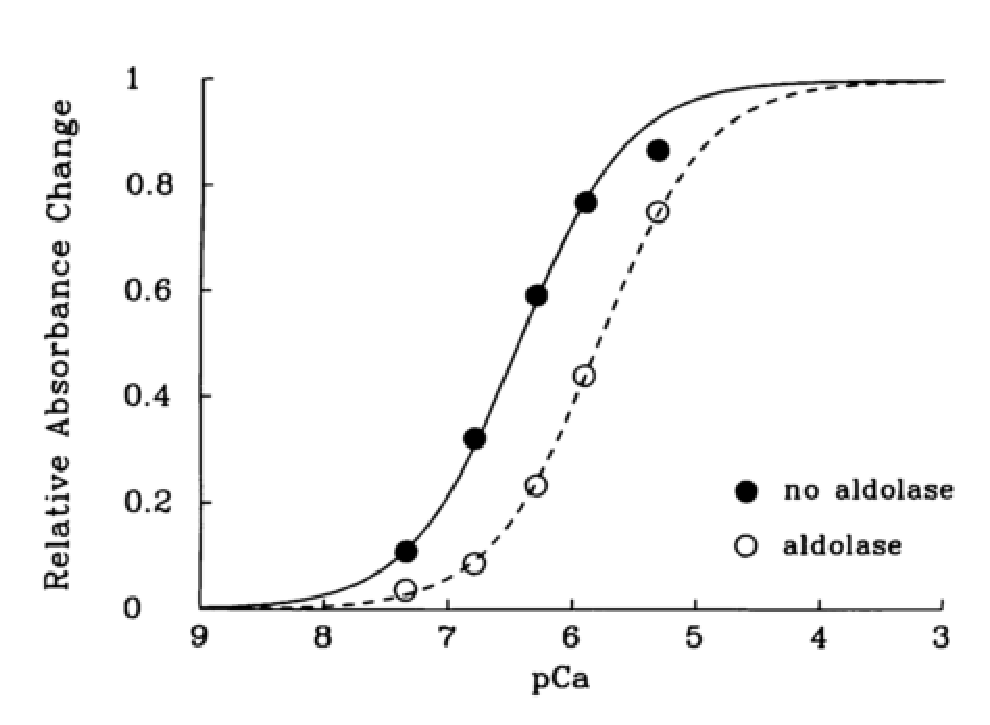
\includegraphics[height=4cm]{./images/Kd_Furared_kurebayashi93.eps}}
\caption{Relative amplitude of Fura red at different calcium level. Each curve
is the least-square fit of 1:1 binding curve. The best fit of $K_D$ was
0.36$\muM$ (without aldolase), and 1.59$\muM$ (with aldolase)}
\label{fig:Kd_furared_kurebayashi93}
\end{figure}

The apparent diffusion constant of Fura red {\it in vivo} was estimated about
16$\mum^2/s$, while the expected value is about 100$\mum^2/s$.  It means that a
large fraction of indicator was bound to relatively immobile myoplasmic
constituents. $f_r$ is the fraction of Fura red in $\Ca$-bound form in resting
fibers, which was estimated about 0.15. So, the resting free $[\Ca]_\rest$ was
estimated about 0.19-0.28$\muM$. This range is higher than previous
measurements. Previous measurements showed $[\Ca]_\rest =50$nM (cut fiber) and
less than 60nM in intact fibers; peak $\Delta [\Ca]$ in a single AP is
20-30$\muM$ (cut fiber) and 10-15$\muM$ (intact fibers).

\subsection{Harkins-Kurebayashi-Baylor (1993) - skeletal muscle}

\citep{harkins1993} studied the resting calcium level in skeletal muscle using
Fluo-3, with experiments at 16-17$^\circ$C. Previously, studies used aequorin
(Sect.\ref{sec:aequorin}) and $\Ca$-selective microelectrodes estimated $[\Ca]_\rest$
in the range 0.02-0.12$\muM$. 

Data from experiments using Fura red showed a higher resting value 0.2-0.3$\muM$
\citep{kurebayashi1993} (Sect.\ref{sec:kurebayashi1993}). To estimate free
$[\Ca]_i$, a novel calibration method was suggested with Fluo-3.
The results support the conclusion that $[\Ca]_\rest$ is at least 0.1$\muM$ and
can be as large as 0.3$\muM$. \citep{harkins1993} estimated different factors
that may affecting the measurement of $\Delta F/F$ signal.

The {\it in vivo} $K_D$ was estimated using the formula
\begin{equation}
\label{eq:Kd_harkins}
\frac{F-F_\min}{F_\max-F_\min}= f = \frac{[\Ca]}{[\Ca]+K_D}
\end{equation}
with $K_D$ was chosen so that the right-side fit to the data in the left-side;
$F$ is the fluorescence intensity (fluorescent of calcium-bound
fluorescence under 1:1 binding ratio CaF).

The resting fluorescent $f_r$ measured just prior to stimulation which is
related to $F$ in the form
\begin{equation}
F = F_\min + f_r \left( F_\max - F_\min \right)
\end{equation}
with $F_\max, F_\min$ are intensity levels that can be measured if all the
indicator molecules in the measurement region were either $\Ca-$bound or
$\Ca$-free, respectively. In other words, $F_\max $ is the saturation level of
CaF, and $F_\min$ is the self-fluorescent of Fluo-3 itself. [NOTE: In
simulation, we can safely set $F_\min=0$, $F_\max=\ldots$].

Also, $\Delta F$ is related fo $\Delta f$ by
\begin{equation}
\Delta F= F - F_\min = \Delta f \left( F_\max - F_\min \right)
\end{equation}
with $\Delta f = \Delta[CaF]/F_T$

To estimate $K_D$, they assumed, as shown in Fig.\ref{fig:fluo3_harkins93}(A)
\begin{enumerate}
  \item binding of dyes to protein (aldolase), forming PD, $K_2$
  \item binding of $\Ca$-bound Fluo-3 (CaD) to protein, forming CaPD with
  $K_{1}$
  \item binding of $\Ca$ to dye, forming CaD with $K_{D1}$
  \item binding of $\Ca$ to protein-dye complex, forming CaPD with $K_{D2}$
\end{enumerate} 
PD has a lower affinity to $\Ca$ than free dye, i.e. $K_d=$1.92$\muM$ vs.
0.51$\muM$, respectively. CaD has a lower affinity for protein than free dye,
i.e. $K_d=1378\muM$ vs. 366$\muM$, respectively.  When $\Ca$ is released, CaD
rises. The loss of dye D is compensated by the unbinding of dye from its
protein-bound form (PD$\rightarrow$ P + D). The dynamics increase of D, and
the greater diffusion of CaD over CaPD should decreases the amplitude and
broaden the spark. 

\begin{figure}[hbt]
 \centerline{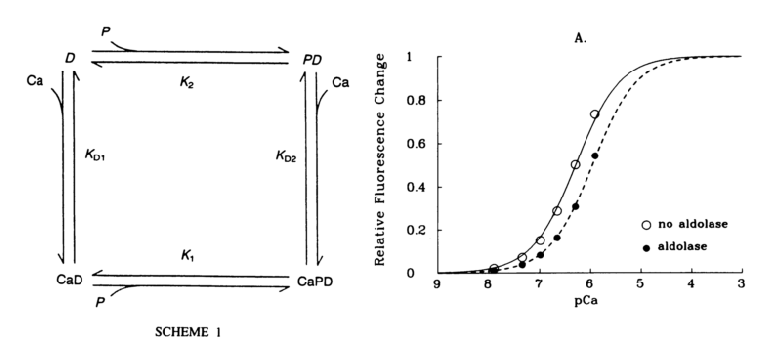
\includegraphics[height=4cm]{./images/Fluo3_harkins93.eps}}
\caption{(A) Schematic diagram of Fluo-3 in the system; (B) Estimation of
fluorescence in solution of the indicated pCa minus that measured in zero
$[\Ca]$ in solution, with and without aldolase}
\label{fig:fluo3_harkins93}
\end{figure}


In the absence of 55mg/ml Aldolase, $K_D=0.51\muM$ (prevously \citep{4} reported
as 0.40$\muM$). Using these information, we assign $K_{D1}=0.51\muM$ and
$K_{1}=1.378$mM. Using the law of mass action, it requires $K_{D2}\times K_2 =
K_1\times K_{D1}$. Then, under the assumption $K_2\times K_{D2}=703 \muM^2$),
using least-square fit, Fig.\ref{fig:fluo3_harkins93}(B), $K_2=336\muM$,
$K_{D2}=1.92\muM$.

If we implicitly consider aldolase in the system, the effective single-site
$K_D=1.09\muM$, which is between $K_{D1}$ and $K_{D2}$. This value of $K_D$ was
2.1x higher when without Aldolase. The inrease here is somewhat less than that
reported in Fura-2 and fura-red, where the factor is 3.3 and 4.4, respectively.
The best fit of $k_+=15.2 \muM^{-1}$, and $k_{-}=37.5$s$^{-1}$, with
$K_D=k_-/k_+=2.47\muM$. For the fit, $f_r $ was assumed to be 0.082, and
$[\Ca]_\rest=0.22\muM$.

The total concentration of dye ($D_T$) is also unknown. A table of different
estimation was given in Tab.5 of the paper. In
Fig.\ref{fig:fluo3_transient_harkins93}.

\begin{figure}[hbt]
 \centerline{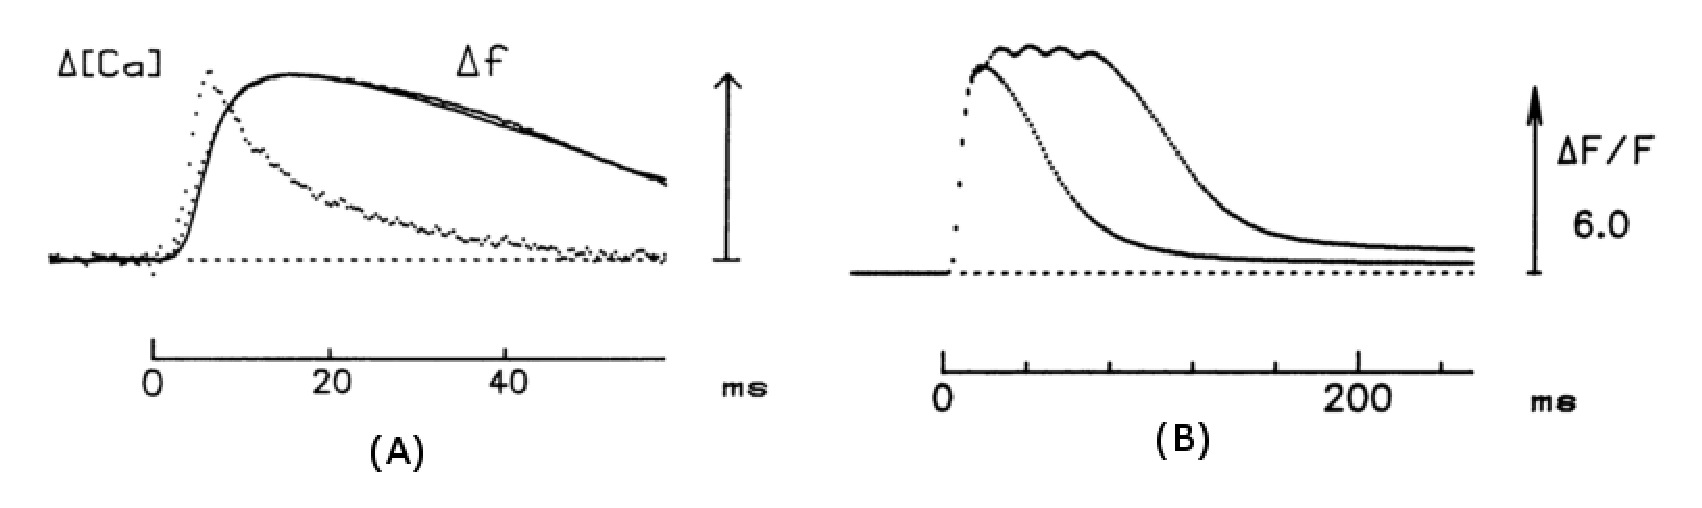
\includegraphics[height=3cm]{./images/Fluo3_transient_harkins93.eps}}
\caption{(A) The peak $[\Ca]_i$ was 15.3$\muM$. The peak $\Delta f$ was assumed to be 0.656
(with $\Delta F/F=7.3$). (B) Fluorescent changes in response to one shock or a
train of five shocks separated by 15ms.}
\label{fig:fluo3_transient_harkins93}
\end{figure}


\subsection{Cheng et al. (1993)}
\label{sec:spark_cheng1993}

~\citep{cheng1993cse} first recorded local elevation of calcium in quiescent
cardiac cells using fluorescence Fluo-3 and line-scanning confocal microscopy,
Figure.\ref{fig:spark_Cheng1993}. $\Ca$ sparks is the term to coin this
elementary event. \textcolor{red}{$\Ca$ sparks evoked by depolarization were not
actually observed at this time} (Sect.\ref{sec:lopez-1994}).
The spark reflect spontaneous calcium release in small regions of the cell, with
frequency 1.3 spark/sec in a thin ($<1\mum$) confocal image section of the cell.
There was no sparks observed using Ryanodine $>1\muM$, which suggest RyR is the
calcium release channels of $\Ca$ sparks, while reducing ryanodine concentration
down to 100-300nM, the spark rate increase from 1.6 to 3.53 sparks per line-scan
image.

The region of local increase $[\Ca]_i$ appeared to restricted into a circular
area with diameter 3.0$\mum$. The line-scan data showed that the elevation time
to peak is about 10ms (the same as evoked transient), and the half-time decay
($t_{1/2}$) is 22.3$\pm$1.12 (ms) (while decay of evoked transient is slower,
164ms). The peak of a normal $\Ca$ sparks is between 200 to 300 (nM). The small
sparks have peak $\sim 200$ (nM) and macro sparks have peaks $\sim 533$ (nM).
The free calcium is calibrated using the method described in
Sect.\ref{sec:cheng-et-al_subsect}.

\begin{figure}[hbt]
  \centerline{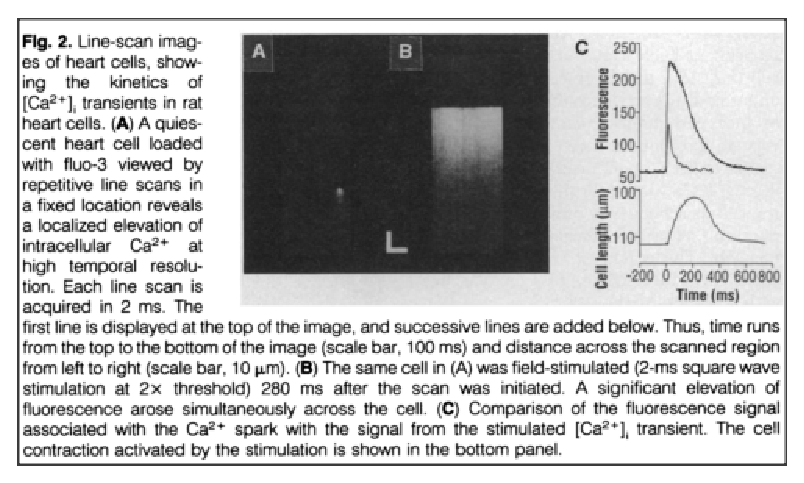
\includegraphics[height=5cm,
    angle=0]{./images/spark_Cheng1993.eps}}
\caption{Line-scan image of $\Ca$ sparks}
\label{fig:spark_Cheng1993}
\end{figure}

They also observe low-amplitude spark of long duration which may suggest RyR
open at sub-conductance state. However, \textcolor{red}{not many computational
works incorporate this subconductance state}. The opening rate at rest is very
low (0.0001 s$^{-1}$), which gives 100 sparks/cell/second. In a spark, the
estimated $[\Ca]_i$ increase in a region of 2$\mum$ across was $\sim 270$ nM,
compared to the resting value 100nM, the half-time decay time is $\sim 25$ms.
Under $\Ca$ overload (increasing SR $\Ca$ content by using high $[\Ca]_o=10$
(mM)), the opening rate increases 4x, and can trigger $\Ca$ wave. At the
point where the wave start, a 'macrospark' occurred, with the peak of about
533nM. The speed of $\Ca$ wave was detected as 70 ($\mum$/s).

The flux of $\Ca$ release is modelled as
\begin{equation}
J = \beta.\Delta[\Ca]_i . V. T^{-1}
\end{equation}
with $\beta = 100$ is buffering power of the cell for $\Ca$ released; 
% (defined as
% $\frac{[\Ca]\text{ release}}{[\Ca]\text{ increased}}$); 
$\Delta[\Ca]=0.2 $ ($\muM$) is concentration  change during the spark, $V=10$fl
(volume of the subspace); and $T=10$ (ms) is the time taken for the rise of
$\Ca$. So $J=2\times 10^{-17}$ (mol/s) or $2\times 10^{-11}$ ($\muM$/s). This
corresponds to total RyR current  to be 4 (pA). Early experimentally
data showed that single channel current $i_{1ryr}=3$ (pA) at 0 (mV). So, they
suggested $\Ca$ spark is the result of opening/closing of a single RyR channel
(or a small number of channels acting in concert).

\subsection{Lopez-Lopez et al. (1994)}
\label{sec:lopez-1994}

\textcolor{red}{\citep{lopez-lopez1994} now show $\Ca$ sparks recorded under
membrane depolarization condition}, in a volume of 2$\mum^3$ (other
studies:\citep{cannell1995b}).
They provided additional data to support the idea that $\Ca$ transient is the
summation of stochastic, independent local events, similar to $\Ca$ sparks. The
difference in these local events were accounted for the difference in the size
of the unitary $I_\Ca$.

All experiments were done at room temperature (21-23$^\circ$). Here, Bio-Rad
MRC-600 line-scanning confocal imaging system was used with Fluo-3 excited at
light 488nm, and measured at wavelengths greater than 515nm. The objective lens
was a plan-apo, oil-immersion lens of magnification x60 and numerical aperture
NA=1.4 (Nikon Inc.). The {\bf line-scan image} is a 2D picture with x-axis is
time, y-axis is the spatial information. The analog recording on each line (i.e.
fluoresence at a fixed time point at different location on a single line) were
digitized into 768 pixels, giving pixel dimensions of 0.271$\mum$, and
2.60$\mus$. It means each pixel represent fluorescence within 0.271$\mum$ region
in wide, measured within 2.60$\mus$. It takes 2ms for scanning the whole-line
and moving the probe back to the original position for the new scan. By scanning
512 times, the data is recorded duging the time period of 1.024(sec). If we
extract one line along the x-axis, we get the {\bf line $[\Ca]_i$ transient }
plot.
 
\begin{framed}
The reason of choosing 768 pixels per line in spatial is that if it takes
2.6$\times 10^{-3}$ (ms) to record a pixel, and the number of pixel is $n$. So,
with the interval of 2(ms) for the next line, this time is enough to record
$n=2/(2.6\times 10^{-3})\approx 768$ (pixels).
\end{framed}

Under that condition, the optical section (z-axis) is about 1.0$\mum$, and the
point being scanned is limited by the diffraction limit 1.0$\mum$. It means
that the recorded pixel actually contains fluorescence arising from points as
far away as 1.0$\mum$ in depth, and 0.271$\mum$ in wide. Typically, a single
pixel in the line is approximated as the fluorescence within the volume
1$\mum^3$.
 
For the quantification of local $\Ca$ transient using the so-called {\bf line
$[\Ca]_i$ transient} at a single point, each new pixel on this line represent
the $[\Ca]_i$ during 2ms (not 2$\mus$). Rather than using the center value, the
new pixel value is the averaged from 4 adjacent pixels along the scan-line.
So, the final pixel represent the averaged fluorescence within a region of
volume 2$\mum^3$ with temporal resolution 2ms per pixel.
 
The result also support the idea that global $[\Ca]_i$ transient is the result
of the summation of local events triggered by unitary $I_\Ca$ currents. It has
been shown that $I_\Ca$ at negative membrane potential (e.g. -30mV) is more
efficacious to induce SR $\Ca$ release that that at positive membrane potential
(e.g. +40mV).
This is coined as {\bf variable gain} \citep{niggli1990,wier1994lce}. The former
is related to low $P_o$ but large unitary $I_\Ca$ current, while the latter is
related to high $P_o$, but small unitary $I_\Ca$ current. In both cases, if the
total $I_\Ca$ influx is the same, but the transient is smaller in the latter
case, then it can be inferred that either the local $\Ca$ transient is smaller
or less frequent. \textcolor{red}{It was wrongly to choose the first
hypothesis}. Later, it will be shown that the spark characteristic is
independent from the $\Ca$ influx. So, it must be the less frequent of spark 
triggering in the case of positive potential.
 

\subsection{Cannell-Cheng-Lederer (1994)}

Previous studies using wide-field microscope weren't able to resolve the spatial
non-uniformities of $\Ca$ transient. Another factor that limit the capabilities
is the short period of time where non-uniformity of $\Ca$ transient occur
(within 10ms) while the conventional image acquisition time is $\sim 30$ ms.
\citep{cannell1994snu} showed that $\Ca$ sparks at different CRUs are not
triggered at the same time upon depolarization. Even at the same time, the delay
varies from beat to beat. \textcolor{red}{This suggest a stochastic nature of SR
$\Ca$ channel activation}. This non-uniformities are enhanced by the adding of
$\Cd$, suggesting the primary sources of spark activation is the current through
LCC.
In overall, this suggests stochastic gating of channels play a major role in
spark initiation/termination and models of EC-coupling should consider
stochastic behavior to adequately describe behavior at sarcomeric and
subsarcomeric levels.

Bio-rad MRC 600 line-scanning confocal imaging system. The objective lens is
Nikon Neofluor 40x NA=1.3. The axial resolution (z-axis) is 0.8$\mum$ and x-y
resolution is under 0.4$\mum$ as measured at FWHM with 0.1$\mum$ fluorescent
beads. Using Fluo-3 with excitation wavelength 488nm. 

STIMULATION PROTOCOL: 2ms voltage pulse with the stimulation pulse set to 1.5x
threshold. 

\subsection{Lopez-Lopez et al. (1995)}
\label{sec:lopez-lopez-et}

D 600, a methoxyl derivative to verapamil, can reduce the mean open channel
lifetime and the frequency of opening without changing the amplitude or the
length of time until the first opening observed (i.e. not chaning first latency)
\citep{mcdonald1989}. ~\citep{lopez-lopez1995} used verapamil to reduce $P_o$ of
LCC, but keep the amplitude of single channel and the same first latencies
(about 0.2ms).
With 10$\muM$ verapamil, using voltage clamp (with holding potential -40mV) with
depolarization during 200ms and $V_\stim$ vary from -30mV to +100mV (with
increment +10mV), local $\Ca$ transient has been observed without cell
contraction at all pulse potential. The result shown no effect of potential on
amplitude and image area could be detected, i.e. the peak 201$\pm$8.86 nM, and
image area 104.8$\pm$4 pixels (Fig.2 of the paper) which is similar to
spontaneous $\Ca$ sparks observed in \citep{cheng1993cse}
(Sect.\ref{sec:spark_cheng1993}).

\begin{framed}
The area is defined as the number of pixels at which the $[\Ca]_i$ exceeds the
half-amplitude of the spark. The latency (waiting time) is measured as the time
elapsed from the onset of the pulse depolarization to the time at which
$[\Ca]$ reaches the peak and then minus 5ms (which is the averaged time to
peak). 
\end{framed}

\begin{figure}[hbt]
  \centerline{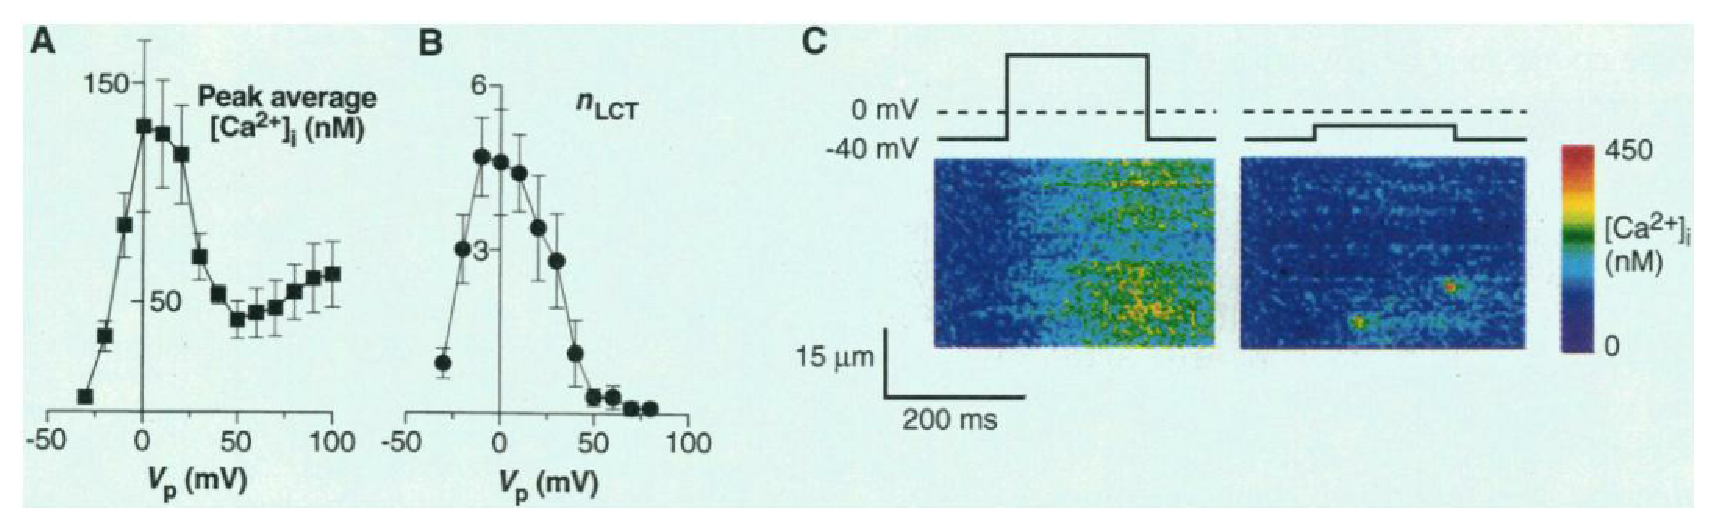
\includegraphics[height=3cm,
    angle=0]{./images/lopez-lopez_spark1995.eps}}
  \caption{(A) Peak average local $[\Ca]_i$ transient vs. $V_m$; (B) number of
  local transient vs. $V_m$; (C) Sparks are obvered more at moderate $V_m$,
  rather than at high positive $V_m$}
  \label{fig:lopez-lopez_spark1995}
\end{figure}

Tested with different pulse potential, ~\citep{lopez-lopez1995} shown that most
local calcium ($[\Ca]_\ds$) was evoked within 40ms. The number of evoked local
$\Ca$ transient decrease rapidly during the pulse potential from -20mV to +10mV
which can be fitted by an exponential distribution with $\tau_{LCT}$. It's
unclear for the relationship at pulse potential more negative or more positive
than this range. 

To compare the time course of single LCC opening (e.g. the slow componentn
$\tau_s$ of inactivation of LCC at 20-25$^\circ$) and the time course of this
latency $\tau$, generally, $\tau_{LCT}$ is smaller than $\tau_s$; yet both have
U-shaped when plotting with $V_m$. So, $\tau_\LCT$ is $V_m$-dependent like
$\tau_s$ of L-type $\Ca$ channel. $\tau_s$ vary from about 550ms at $V_m=-10$mV,
$\tau_s=100$ms at +10mV, and $\tau_s=250$ms at +30mV.

% At more negative or more positive, the time constant is
% less than, yet not sure if can be fitted by exponential.

They suggested that the amplitude of $i_{1\dhpr}$ is important in probability of
triggering evoked spark. At a particular voltage, the relative probability for
trigger a spark $P_\LCT$ is calculated as
\begin{equation}
  \label{eq:1420}
  P_\LCT = \frac{n_\LCT}{n_{\LCT,max}}
\end{equation}
with $n_{\LCT,\max}$ is the total number of local $\Ca$ transients
that occur at a selected potential, e.g. +10mV, and $n_\LCT$ is the number of
events at a particular latency bin of the histogram at that potential.
Another way to calculate this value is
\begin{equation}
  \label{eq:1421}
  P_\LCT = k . P_{i,\LCT}.P_{o,L}
\end{equation}
with $P_{o,L}$ is the prob. a single LCC open, $P_{i,LCT}$ is the
prob. that the influx current will trigger the SR $\Ca$ release, and
$k$ is the scaling factor to make $P_\LCT = 1$ at pulse -40mV.

As shown in Fig.\ref{fig:lopez-lopez_spark1995}, the $[\Ca]_i$ follow the
bell-shaped relationship with the $V_m$ from -50mV to +50mV. Due to the biphasic
dependency of $I_\Ca$ on $V_m$, the influx is smaller at very positive membrane
potential, which is the causes for the lower global calcium transient. At very
high positive $V_m$, the increase in peak $[\Ca]_i$ is the result of $\Ca$ entry
through $\Na/\Ca$ exchanger (NCX). However, the peak is still lower than
that at 0mV. It means that the influx of $\Ca$ through LCC is more effective in
triggering local $[\Ca]_i$; while the high potential is effective in trigger
calcium waves.

\subsection{Cannell-Cheng-Lederer (1995)}



\begin{figure}[ht]
  \centerline{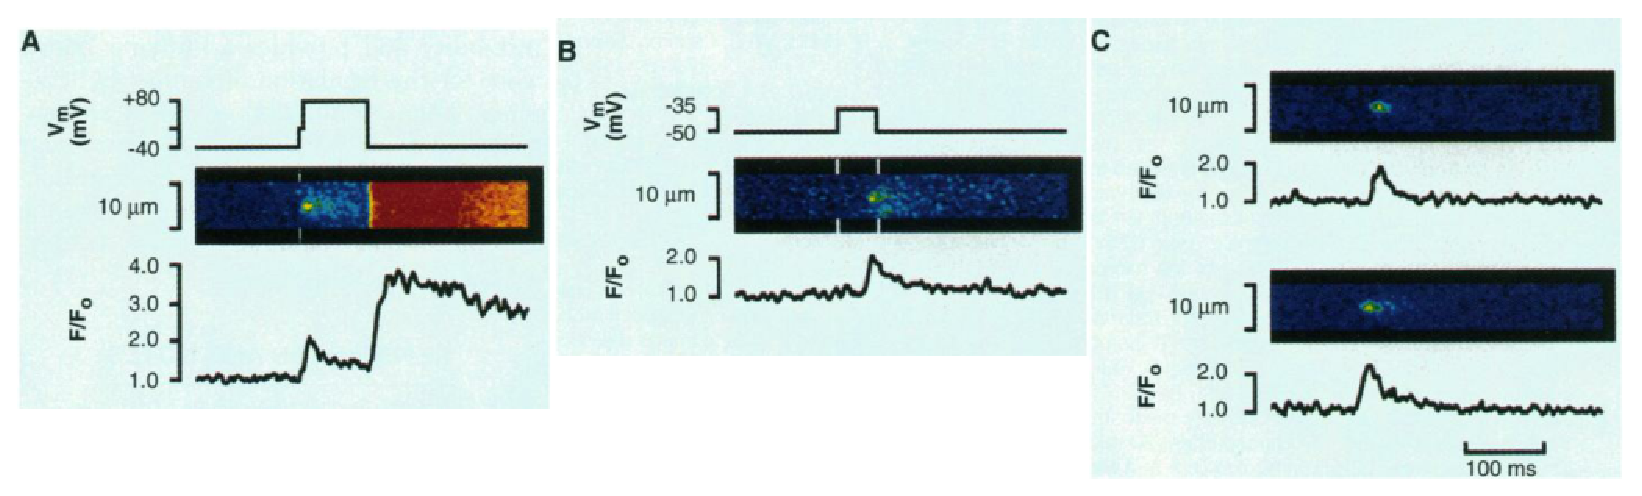
\includegraphics[height=3.5cm,
    angle=0]{./images/spark_cannell1995.eps}}
    \label{fig:spark_cannell1995}
    \caption{(A) Depolarization from -40mV to -5mV for 0.75ms can trigger a
    spark with a latency less than 2ms. The peak F/F0 was 2.08 at 10ms. The
    more positive potential +80mV trigger the global transient. (B)
    Depolarization from -50mV to -35mV trigger a spark with latency 32ms. The
    peak was 2.07 at 10ms. (A) Spontaneous $\Ca$ sparks at holding potential
    -80mV with 100$\muM$ $\Cd$ to block $I_\Ca$; the peak F/F0 was 2.18 at
    10ms}
 \end{figure}
    
Fig.\ref{fig:spark_cannell1995} shown almost similar $\Ca$ sparks
characteristics at different conditions (evoked and spontaneous). In Fig.(B) the
small depolarization is used to trigger only single LCC channel opening, and the
high latency can be accounted for the small $P_o$ of LCC. So, it's suggested
that the spark triggering probability is dependent upon the influx of $\Ca$, but
the spark characteristics (amplitude, duration, kinetics, spatial size) is
determined by the intrinsic gating of RyRs channels. Under normal condition, the
$\Ca$ sensitive of RyR is very low, and can be increased under
hyperphosphorylation settings.

\section{Pratusevich-Balke (1996)}
\label{sec:prat-balke-1996} 


~\citep{pratusevich1996} aimed to create a model that can be used to create a
theoretical-line scan images of an idealized $\Ca$ sparks.
The theoretical image is generated using the 3D data from the simulation,
convolved with a three-dimensional point-spread function (PSF) for each time
point. Also, to make the image looks more realistic, noise is added.

AIM: A major challenge in quantifying $\Ca$ sparks is the unknown position of
spark origin. So, the variation in spark amplitudes can be due to the unaligned
position of the focused laser beam with the center of the CRU. They explored the
effect of photon noise and out-of-focus events on the fidelity of the $\Ca$
spark measurements.


\subsection{Hypothesis analysis}
\label{sec:hypothesis-analysis-12}

The model is developed based on certain assumptions:
(1) all endogenous buffers and exogenous buffers are assumed stationary, (2)
only contractile regulatory protein Troponin-C (endogenous) and Fluo-3
(exogenous) are buffers, with single binding site, (3) not whole-cell, but
subcellular regions was simulated, (4) there is no $[\Ca]_{ds}$ incorporated,
(5) closed-cell simulation (no net flux across plasma membrane), (6) SR $\Ca$
release is assumed from a single source (with square pulse).
 
% \subsubsection{PSF}
% \label{sec:psf}
%  
% Using Nikon Diaphot TMD inverted microscope to which Bio-Rad MRC-600
% confocal imaging system is attached,
% The objective lens is planar-apochro-mat oil-immersion 60x magnification and
% NA=1.4. The lens can move in the z-axis with the step of 0.02$\mum$.
% 
% The PSF is measured by imaging a fluorescent bead 0.1$\mum$ in diameter, taking
% 16 optical sections along the z-axis with 0.28$\mum$ interval. The pinhole
% diameter is 2.5mm, providing a trade-off between the axial resolution and the
% signal collection. As a result, the measured PSF is
% highly asymmetric, with FWHM is 0.48 $\mum$ in the $y$ dimension
% and 1.30$\mum$ in the z-dimension. These values are smaller than those in
% conventional epifluorescence microscopes.

The main source of noise in a confocal microscopy system is the shot noise of
photomultiplier tube~\citep{sheppard1992}. The noise was simulated simply by adding a normally
distributed r.v. at each spatialtemporal point of $[\CaF]$, so that the addition
doesn't change the mean of the signal and the std. was proportional to the mean
wih a coefficient. The proportionality coefficient (usually 0.5) was varied
until the appearing of the constructed image similar to experimental record. The
PSF being used is FWHM$_{x,y}=0.48\mum$, FWHM$_z=1.30\mum$.
 
\subsubsection{Simulated cell volume}
\label{sec:simul-cell-volume}



\begin{figure}[ht]
  \centerline{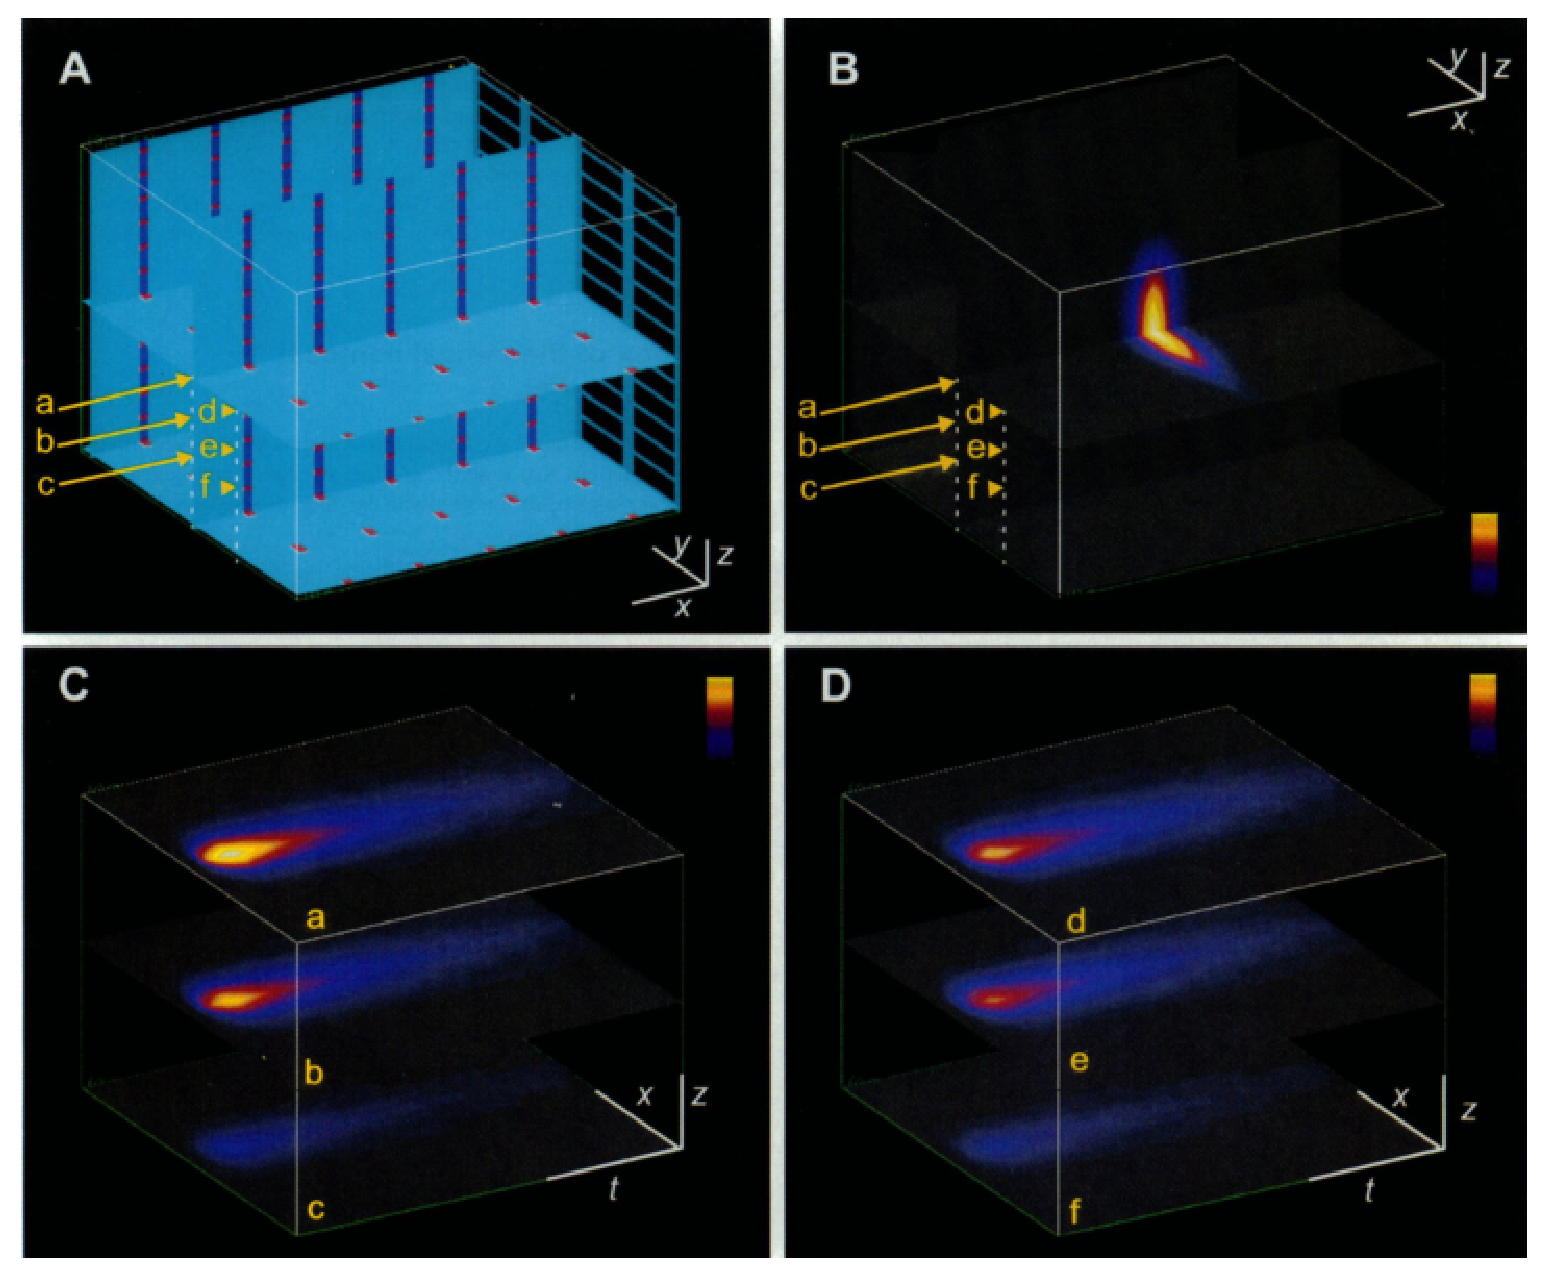
\includegraphics[height=9cm,
    angle=0]{./images/pratusevich_spark2.eps}}
  \caption{A view of $\ca$ sparks from different scan lines. (A)
    subcellular schematic diagram: T-tubules are magenta bars; CRUs
    are red elements on magenta bars; SR, in which $\ca$ uptakes
    occurs, are blue elements. (B) 3D confocal image. (C)-(D) six
    different views of $\ca$ sparks as if (a) scanning through the
    origin of $\ca$ sparks, (b) defocused (displayed downward) by
    1.08$\mum$, and (c) 2.16$\mu$m; and (d-f) displaced literally by
    0.54$\mum$ with the same depth as in (a-c). NOTE: Calibration bars in
    (A-B): x=2.16$\mum$,y=0.68$\mum$, z=1.35$\mum$; in (C-D): t=50ms,
    x=2$\mum$, z=0.54$\mum$.
    \textcolor{red}{The color scale span the range of ratio $F/F_o$
      from 1.0 to 3.0 (estimated $[\ca]_i \sim 100$ to 364 nM)}}
  \label{fig:pratusevich_spark2}
\end{figure}
\clearpage

Due to the highly computational demand to simulate the whole-cell, a
subcellular region of the mammalian ventricular myocyte was simulated.
\textcolor{red}{The volume need to be large enough so that both PSF
  and $\Ca$ image could decay to values well below a fraction of
  percent of their respective maximum level, at the borders of the
  simulation space}.  So, they chose an area equivalent to
\begin{itemize}
\item 6.5 sarcomeres long (x), -6 sarcomeres wide (y), and 17
  sarcomeres depth (z).

\item or equivalent to the volume of size 11.92 $\mum$ x 2.97 $\mum$ x
  8.64 $\mum$ (in the x, y, and z directions, respectively).
\end{itemize}


\subsubsection{Buffers}
\label{sec:buffers-2}

It's assumed that $\ca$ binds only to dyes (Fluo-3) and a single
endogenous buffer (ligand or Troponin-C), following the law of mass
action with single binding site.  \def\lig{{\text{lig}}}
\def\dye{{\text{dye}}}
\begin{equation}
  \label{eq:1116}
  \begin{split}
    \ce{Ca + F <=>[k^+_\dye][k^-_\dye] CaF} \\
    \ce{Ca + lig <=>[k^+_\lig][k^-_\lig] Calig} 
  \end{split}
\end{equation}
Both buffers are assumed to be stationary (i.e. $D_F=0, D_\lig=0$)\citep{berlin1994iccb}.
So, the change $d[\ca]/dt$ caused by the binding/unbinding is given in eq.~\eqref{eq:1036}
\textcolor{red}{This work neglect the possibility of diffusion of fluorescence,
and $\Ca$ that was bound to diffusible $\Ca$-binding ligands}.



\subsubsection{Calcium-release site}
\label{sec:calcium-release-site}

They studied spontaneous sparks, so no DHPR was examined. One
limitation is that the cluster of RyR has not been taken into
account. Instead, the SR $\Ca$ release was modeled as a single point
source with rectangular pulse of $\Ca$ current $i_\ca$,
eq.~\eqref{eq:1035}.

\subsubsection{Calcium uptake}
\label{sec:calcium-uptake}

The model of SERCA pumps was based on Michaelis-Menten approach for
simplicity, with Hill coefficient $n=4$
(Sect.~\ref{sec:mich-ment-appr}). So, the change of calcium is given
in eq.~\eqref{eq:1037}.



\subsection{Mathematical model}
\label{sec:mathematical-model-18}

Each voxel on the image is a single grid element in the subcellular
region. The index of the grid element (voxel) are denoted as $(i,j,k)$
in 3D. At each grid element, $\Ca$ involves in (1) binding with Fluo-3
and Troponin-C, (2) diffuse from one grid point
to another; (3) being uptake by SERCA pumps, (4) being released from
the SR. % The dynamics of calcium is given by the sum of components
% associated with diffusion, uptake, and binding to ligands.
\begin{enumerate}
\item Reaction with dyes and endogenous buffer (ligand)
  \begin{equation}
    \label{eq:1036}
    \frac{d[\Ca]_{ijk}}{dt} = k^-_\dye[\CaF] - k^+_\dye[\Ca][\ce{F}] + 
    k^-_\lig[\Calig] - k^+_\lig[\Ca][\ce{lig}] 
  \end{equation}
  Total concentration: Fluo-3 is 50$\muM$, and Intracellualr ligand is 134$\muM$.
To ensure binding reactions is fast enough compared to diffusion, the forward
rate $k^+$ was chosen large enough, $k^+_\dye=k^+_\lig=108\muM^{-1}$.s$^{-1}$.
 $k^-$ are adjusted so that the $K_d=k^-/k^+$ fit to experimental data, i.e.
$k^-_\dye=50$ (s$^{-1}$).
For ligand, $k^+_\lig=108 \muM$.s$^{-1}$, and $k^-_\lig=63$s$^{-1}$.
%   
%   with
%   \begin{itemize}
%   \item $k^-_\dye = 50$s$^{-1}$, $k^+_\dye = 100\muM^{-1}$.s$^{-1}$
%   \item $k^-_\lig = 63$s$^{-1}$, $k^+_\lig = 100\muM^{-1}$.s$^{-1}$
%   \end{itemize}

  We also need 4 ODEs for $[\ce{lig}], [\Calig], [\ce{F}]$ and
  $[\CaF]$.  Initial values for $[\ce{lig}], [\Calig], [\ce{F}]$ and $[\CaF]$ are
  derived from equilibrium with the resting free $[\ca]_i=0.1\mu$M
  (Sect.~\ref{sec:slow_rapid-bufferings}), and $[\ce{F}]_T=50\mu$M,
  $[\ce{lig}]_T=134\mu$M.

\item Diffusion: using Fick's law~\citep{crank1975}
  \begin{equation}
    \label{eq:1034}
    \begin{split}
      d[\Ca]_{ijk}/dt &= D\nabla^2 [\Ca]_{ijk} = \\
      & D_x([\Ca]_{i+1,j,k}-2[\Ca]_{i,j,k}+[\Ca]_{i-1,j,k})/dx^2  \\
      + & D_y([\Ca]_{i,j+1,k}-2[\Ca]_{i,j,k}+[\Ca]_{i,j-1,k})/dy^2  \\
      + & D_z([\Ca]_{i,j,k+1}-2[\Ca]_{i,j,k}+[\Ca]_{i,j,k-1})/dz^2 
    \end{split}
  \end{equation}
  with $D_\Ca=600\mum^2$/s (diffusion of unbound $\ca$ in aqueous
  solution)~\citep{hodgkin1957}
  (\textcolor{red}{next models use a smaller diffusion
    coefficient}). The diffusion of $\ca$ in SR was decreased by a
    factor of 5, i.e. 20\% of the diffusion in the cytosol. We also
    have another ODE for $d\ca_{ijk,sr}/dt$.


\item SR $\Ca$ release is modelled as a rectangular pulse
  $i_\ca=1.4$pA (with duration 12ms) that enter the center voxel from
  an adjacent cell
  \begin{equation}
    \label{eq:1035}
    d[\Ca]_{ijk}/dt = \frac{i_\ca}{F.z_\Ca.U_v}
  \end{equation}
with $F$ is Faraday constant, $z_\Ca$ is the valence of $\ca$, $U_v$
is the volume of the grid element (voxel).
% \begin{eqnarray*}
%   U_v = 0.271\times 0.135\times 0.135 = 4.94e-3 \;\;\;\mu \text{m}^3
% \end{eqnarray*}
Grid elements $dx=0.271\mum$, $dy=dz=0.135\mum$. Voxel volume
$U_v=dxdydz=4.94\times 10^{-3}\mum^3$, Fig.~\ref{fig:pratusevich_spark2}. So,
totally, we have $44\times 22\times 64=61,952$ grid elements (pixels).

\item The SERCA pump is modeled as pump-leak approach using classic
  Hill equation with $\eta=4$
  \begin{equation}
    \label{eq:1037}
    d[\Ca]_{ijk}/dt =
    v_{max}\left[\frac{[\Ca]_{ijk}^\eta}{(K_m)^\eta+[\Ca]^\eta_{ijk}} - \frac{[\Ca]^\eta_\rest}{(K_m)^\eta+[\Ca]^\eta_\rest}\right]
  \end{equation}
  with $v_\max= $ (peak amount of $\ca$ bound to SERCA per unit area
  of SR element $U_a=3.65\times10^{-2}\mum^2$), $K_m=2.89\times10^{-7}$M is
  Michaelis constant.

  The peak amount of $\Ca$ bound to SERCA per unit area of SR element,
  we use
\begin{equation}
  \label{eq:1038}
  v_\max = k_\max.A_p.U_a
\end{equation}
with $k_\max=20$ s$^{-1}$ is SERCA-pump turnover rate, $A_p=5\times
10^{-14}\mu$mol/$\mum^2$ is SERCA pump density. Then $v_\max\approx
44,444\mu$M.s$^{-1}$.


\end{enumerate}


\subsection{Numerical solving}
\label{sec:numerical-solving}

They used a special programming language for finite-difference
approximation call FACSIMILE (AEA Technologies, Harwell,
UK). Mass conservation control (i.e. no net charge in $\Ca$ or other
variables) and no-net-flux boundary condition were used.  The time
steps were automatically adjusted by FACSIMILE; and the output was
sampled at every 2-ms interval, as in experimental line-scan images
obtained by Bio-Rad MRC 600 confocal microscope. Computational and Image
Analysis used IDL. 



\begin{framed}
  These dimensions were convenient because the pixels of our actual
  line-scan confocal images are also 0.271 p.m in x and because the
  voxels of the actual PSF (see below) are integral fractions of
  0.271, that is, 0.068 p.m (x) by 0.068 p.m (y) by 0.271 p.m (z).
\end{framed}

\textcolor{red}{The intra-CRUs distances are 2.16$\mum$ in x and
  0.675$\mum$ in y}.
The SR is assumed to be every where to sequester back the $\Ca$ via SERCA pumps.
Fig.~\ref{fig:pratusevich_spark2} show the simulated volume, in which the SRs
(blue elements in Fig.(A)) are modeled with 2 sets of parallel planes
0.675$\mum$ apart, one is normal to the z-axis, the other is normal to the
y-axis.



% \subsection{Reconstruct theoretical confocal image}
% \label{sec:reconstruct-image}
% 

\subsection{Analysis}
\label{sec:analysis-16}

The color scale F/F0 span the range of 1.0 to 3.0 (estimated $[\Ca]_i$ from
100nM to 364nM), Fig.\ref{fig:F_F0_pratusevich1996}.

The raw image is added with noise first, before applying the convolution
operator with the PSF for blurring. To find the FWHM, the image is smoothed with
a median filter, which decreased slightly the $\Ca$ spark amplitude ($< 3-5\%$).

\begin{figure}[ht]
  \centerline{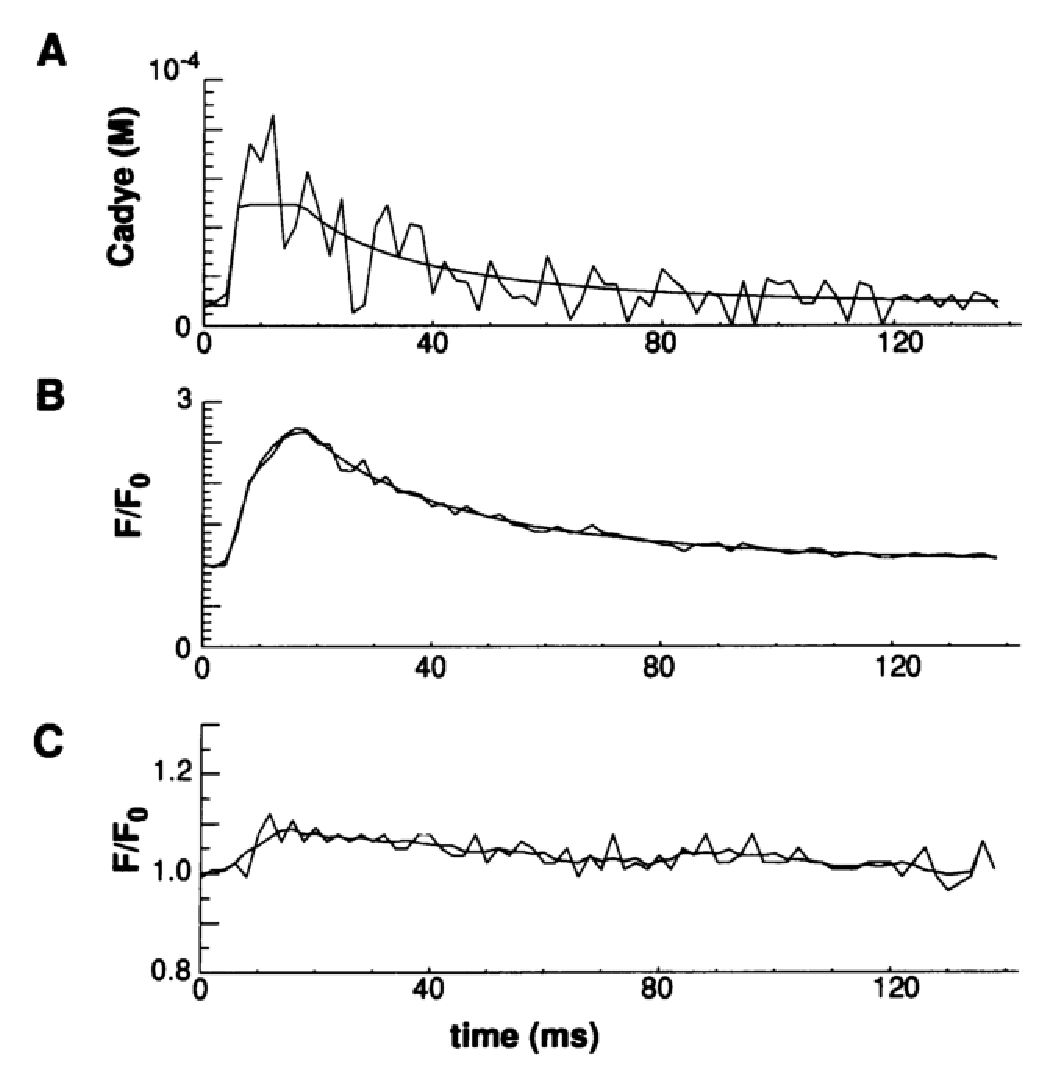
\includegraphics[height=3.5cm,
    angle=0]{./images/F_F0_pratusevich1996.eps}}
    \label{fig:F_F0_pratusevich1996}
    \caption{Simulation with noise, time course of (A) CaF, (B) F/F0 at the center, and (C) F/F0 at the off-center} 
 \end{figure}
 
Using convolution operator, the image was constructed as discrete
convolution of $[\CaF]$ and the PSF
\begin{equation}
  \label{eq:1039}
  I(x,y,z,t)|_{t=t_i} = [\CaF](x,y,z,t)|_{t=t_i} \star PSF(x,y,z)
\end{equation}
with $\star$ denotes convolution operator. To achieve this, we convert
the convolution to multiplication using 3-D Fourier transform of
$\CaF$ and the PSF, which is available in IDL as a procedure. This
requires $[\CaF]$ and $PSF(\cdot)$ has the same dimension and their
voxels are of the same size.
\textcolor{red}{That's why the grid element was chosen of the same
  size as the PSF voxel}.


To produce a line-scan image (i.e. scanning a long a single line in 2D), we need
to go through a number of steps:
\begin{enumerate}
\item extract a single line from 3D data I(x,y,z,t), by fixing $y$ and $z$,
sampling to arrive at a 2D array of intensity of distribution along the $x$ and
$t$ dimensions. 
\item simulate level-adjustment during 8-bit analog-to-digital
  conversion (to bring the simulated image quantatively close to the
  images obtained experimentally) by linear scaling the intensities
  between 0 and maximum value $I_\max$ ($I_\max$ is set above the
  maximal value of $I(x,y,z,t)$. 

  % The new intensities are represented by $F$.
\item mimics the determination of $[\Ca]_i$ from fluo-3 images by
  dividing all image intensity levels by values of resting
  $[\Ca]_{i,rest}$, i.e. $[\Ca]_i/[\Ca]_{i,rest}$. This is the pseudo-ratio
  $F/F_o$ as we assumed that $[F]$ is directly proportional to $[\CaF]$.
  However, it's better to  consider $\Ca$-bound fluorescence and use
  $F/F_o=[\CaF]/[\CaF]_{rest}$.
  
\end{enumerate}
The model predicted a monotomic spark amplitude distribution when the
scan line is positioned randomly w.r.t the origin of the $\Ca$
spark. Result: at $[\Ca]_i$ peak, the FWHM of the image intensity
distribution are 0.74, 1.14 and 2.84$\mum$ in x,y, and z direction
respectively. 

In this model, the author used an unrealistically large value $v_\max\approx
44,444\mu$M.s$^{-1}$ for the SERCA, compared to the value reported
by~\citep{bassani1994rir} 208$\mu$M.s$^{-1}$ In addition, they use a high free
$\Ca$ diffusion coefficient $D_\ca=600\mum^2$.s$^{-1}$. The  explanation is
that the model has not incorporated the mobility of the exogenous buffer
(Fluo-3), which can help spreading $\Ca$ further.~\citep{smith1998} showed
that neglecting this may introduce large errors in the amplitude, time to peak,
relaxation, and spatial spreading of the simulated sparks
(Sect.~\ref{sec:smith-et-al}).


\section{Smith et al. ($\ca$ puffs) (1996)}
\label{sec:smith-et-al-1}

$\Ca$ puffs is the local regenerative release of $\Ca$ via clusters of
IP$_3$R/$\Ca$ channels, followed by
$\Ca$-inactivation~\citep{smith1996}.
\begin{enumerate}
\item for plasma membrane $\Ca$ channels, $[\Ca]_{ds}$ is a function
  of single-channel current which is largely determined by membrane
  potential and external $\Ca$ concentration~\citep{}

\item for intracellular $\Ca$ channels, $[\Ca]_{ds}$ is largely
  determined by luminal $\Ca$ concentration~\citep{}
\end{enumerate}

Cellular $\Ca$ buffers effectively reduce free $\Ca$ concentration,
and localize $\Ca$ signaling by reducing the effective diffusion for
$\Ca$. 

$\Ca$ indicator dyes (e.g. Fluo-3) are mobile $\Ca$ buffers. These
mobile buffers have an additional ``sink'' effect, i.e. further reduce
free $[\Ca]$. 


$\Ca$ buffs were analyzed based on the rapid buffering approximation
near a $\Ca$ source. The used parameters were more relevant to {\it
  Xenopus oocytes}, rather than cardiac cells. The study show an upper
bound on the source strength to produce a given $\Ca$-bound indicator
dye profile.

\subsection{Mathematical analysis}
\label{sec:math-analys}

The local calcium $\Ca_{ds}$ can 
\begin{enumerate}
\item diffuse to the cytosol with diffusion constant $D$: 
  \begin{equation*}
    D\nabla^2[\Ca]_{ds}
  \end{equation*}
\item react with buffers: $\ce{Ca^2+ + B_j <=>[k^+][k^-] CaB_j}$
  \begin{equation*}
    R_j = k^-([B_j]_T-[B_j])-k^+[\Ca][B_j]
  \end{equation*}

\end{enumerate}

\section{Parker et al. (1996)}
\label{sec:parker-et-al}

~\citep{parker1996csi} \textcolor{red}{observed 'subsparks' events (later known
as calcium quarks). They also observed that a spark often involves two or more CRUs
synchronized at a Z-line (due to the nearer distance between them along this
direction) within the delay a few milliseconds}, Fig.\ref{fig:spark_parker1996}.
The last part, they conclude the diffusion of calcium is anisotropic (i.e.
spherically asymmetric), Fig.\ref{fig:spark_parker1996_2}.

\begin{figure}[hbt]
  \centerline{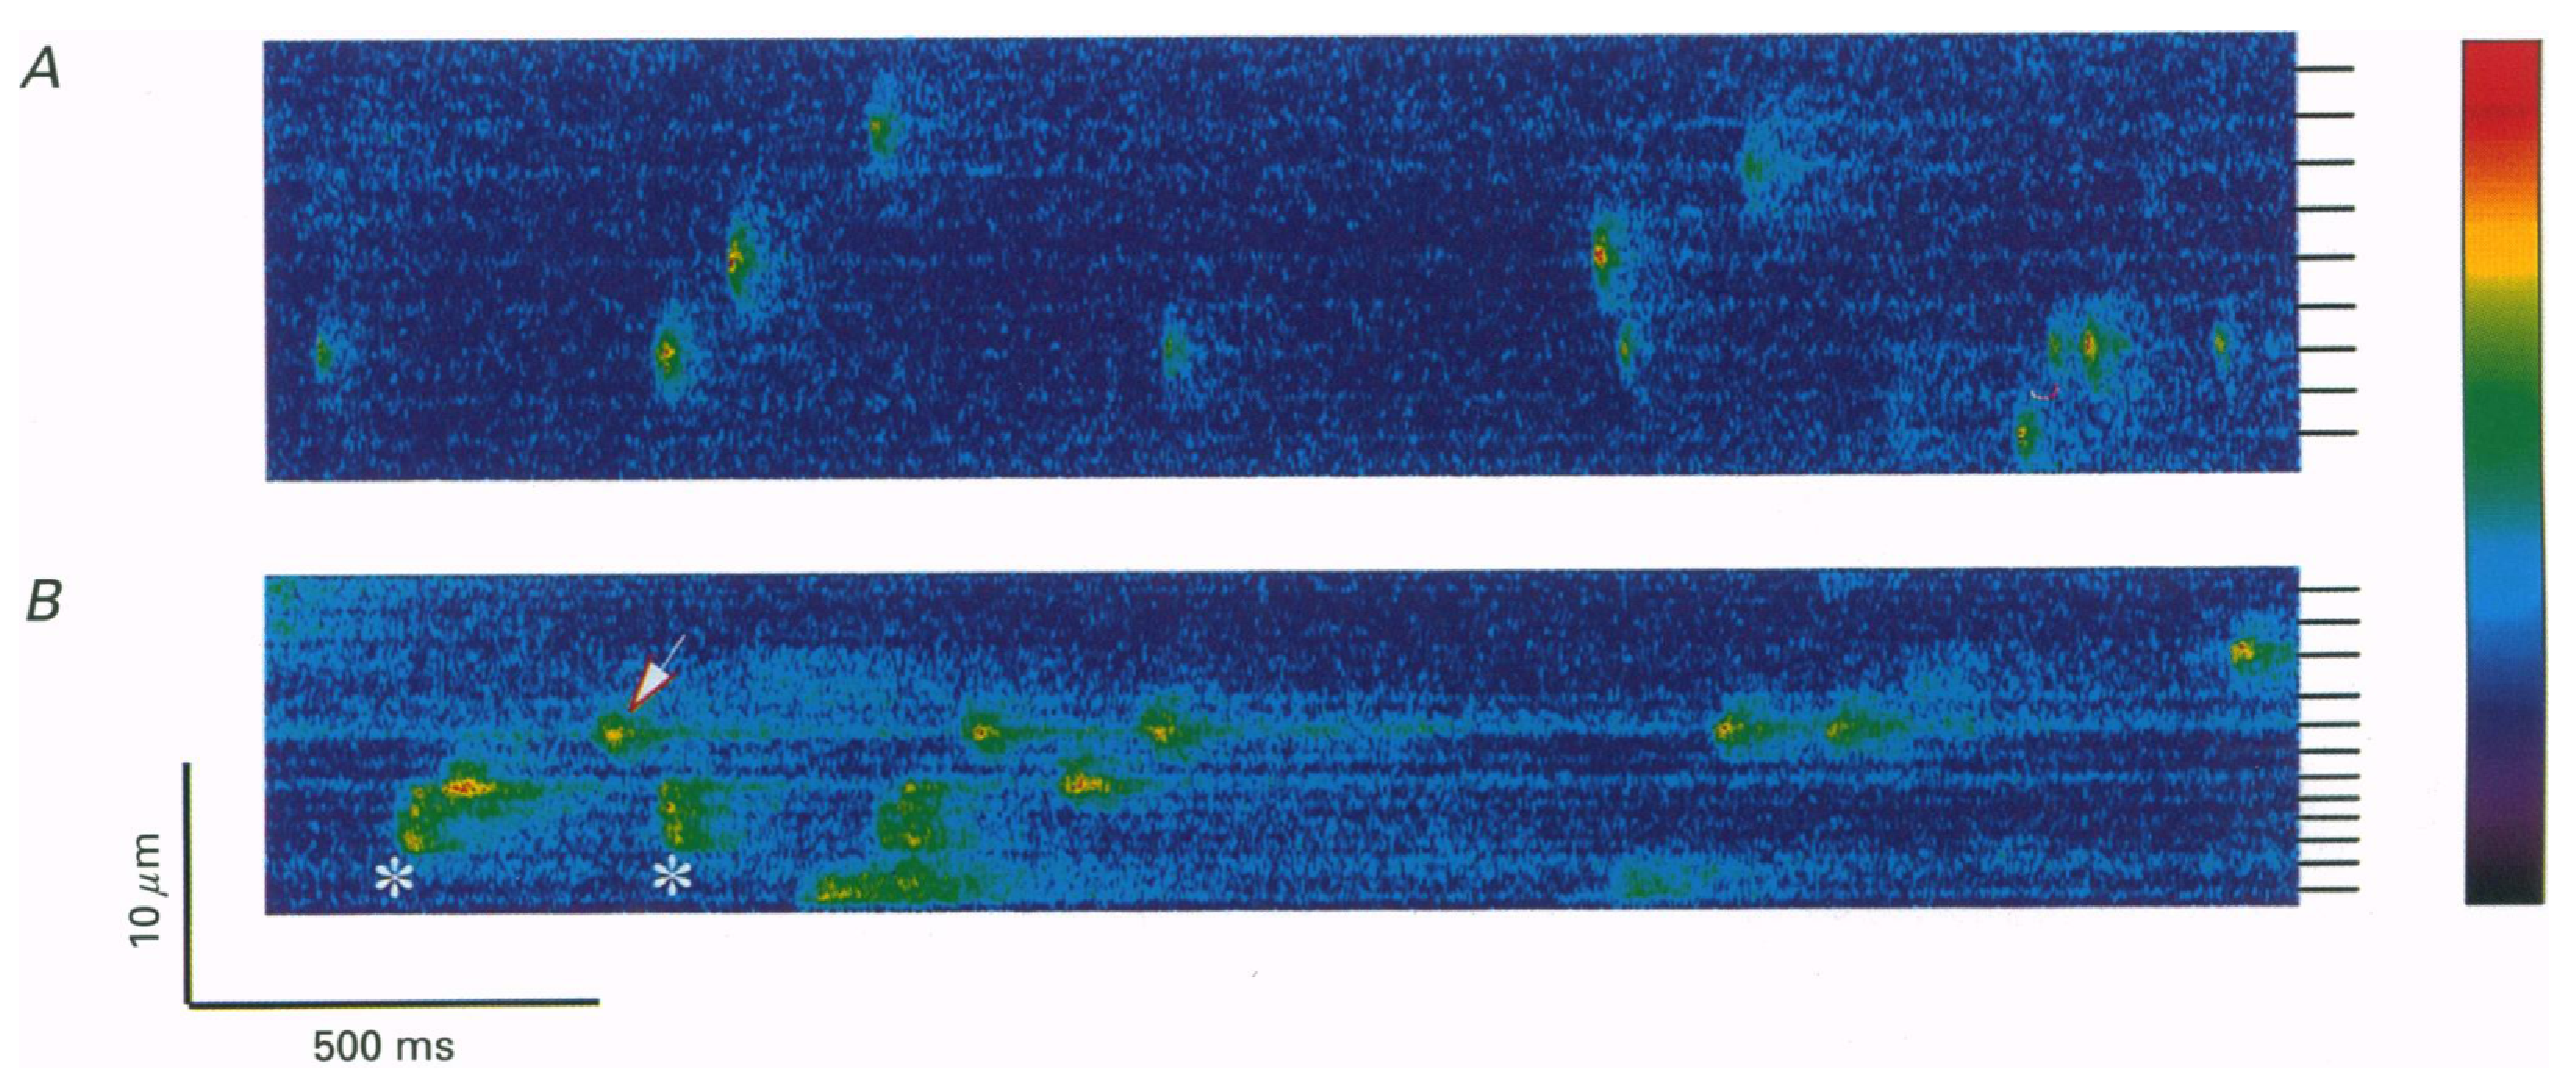
\includegraphics[height=5cm,
    angle=0]{./images/spark_parker1996.eps}}
  \caption{Line at the right mark positions of all CRUs showing sparks
  throughout 15sec recording periods. (A) scan line along the long axis of a
  cell (x-axis); (B) scan line along the trasversal axis (asterisks showing
  synchronized $\Ca$ sparks at multiple CRUs; the arrow indicates $\Ca$ sparks
  at only one CRU.)} 
  \label{fig:spark_parker1996}
\end{figure}

They used ``home-made''  stationary point confocal microscope (with spatial
resolution $\sim 0.3\mum$ in line-scan mode, better than BioRad MRC 600 system,
and sub-millisecond temporal resolution in stationary point mode). Nikon Diaphot
inverted microscope with a x 60 plan-apo oil-immersion objective (NA=1.4) to
transmit only the central of the Airy disk.
This allows continuous recording up to 25sec. The emission wavelength is 488
nm and excited wavelength is $> 515$ nm. The PSF measured using 0.1$\mum$
fluorescent beads was FWHM=0.31$\mum$ laterally and FWHM=0.41$\mum$ axially. The
photon counts was based on 0.1$\mum$ pixel size and sampled at $10\mus$
interval. 5$\muM$ Fluo-3 AM (Molecular Probes, Inc.).

\begin{figure}[hbt]
  \centerline{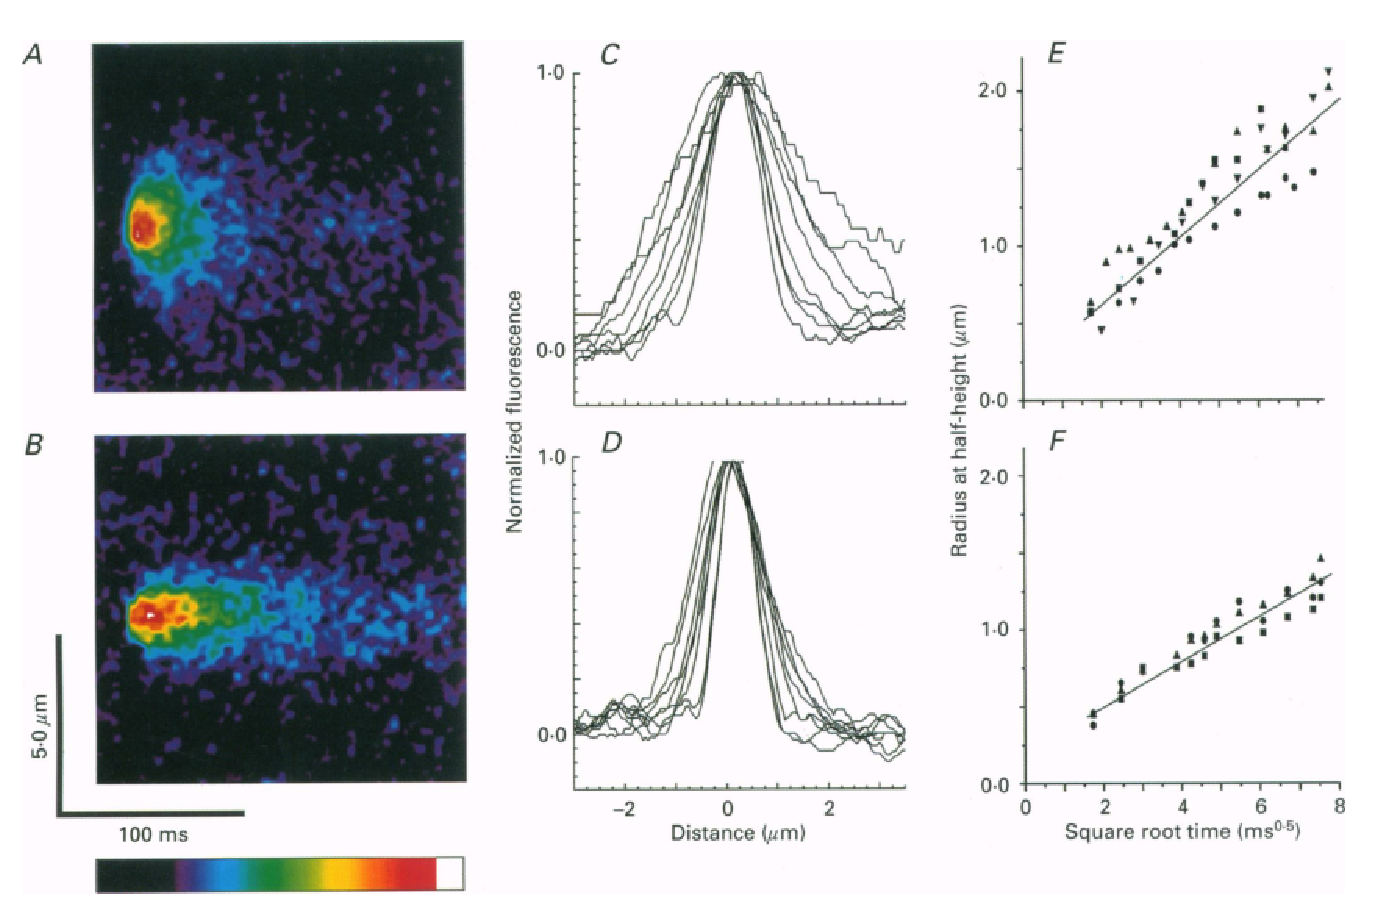
\includegraphics[height=5cm,
    angle=0]{./images/spark_parker1996_2.eps}}
  \caption{$\Ca$ sparks in longitudinal and transversal}
  \label{fig:spark_parker1996_2}
\end{figure}

The single line-scan is about 20$\mum$ long every 3ms. The scan line traject
along the x-axis of the cell or trasversely (parallel to striations). The
fluorescence signal is recorded as $\Delta F/F0$. They model calcium diffusion
as anisotropic with $D_\ca = 17.1\mum^2$/sec in longitudinal and $D_\ca =
7.9\mum^2/$sec in the transversal direction. The values were calculated based on
the formula
\begin{verbatim}
D=(slope)/(-4ln2)
\end{verbatim}
with the slope is derived from the spread of fluorescence signal
(spark profile Fig.2 E and F in the paper). It's properly better reflect the
diffusion of $\Ca$-bound indicator than free $\Ca$. \textcolor{red}{These are
small values compared to those measured recently}. \textcolor{blue}{They
claimed that the diffusion within cardiac myocyte is anisotropic}. Synchronous
activation was not observed between CRUs on different Z-lines (probaly due to
the long longitudinal distance 1.8$\mum$, compared to shorter distance axially
0.76$\mum$).  

\section{Langer-Peskoff (1996)}
\label{sec:Langer-Peskoff_96}

\citep{langer1996} modeled a cleft space as a circular region with radius
0.2$\mum$ and height 0.012 $\mum$, i.e. the volume $1.5\times 10^{-3}\mum^3$.
They modeled 11 LCCs in the cleft. So, with 5500 LCCs in the cell (estimated by
\citep{isenberg1995}), there are 500 clefts. As they assumed 67\% of the cleft
volume is occupied by the feet, i.e. the total cleft volume is
0.25$\mum^3$.

$[\Ca]_\ds$ level reaches 600$\muM$ at the center and 100$\muM$ at the periphery
of the cleft. This is much higher compared to other data. 


\section{Soeller-Cannell (1997)}
\label{sec:soeller-cannell_97}

\citep{soeller1997} \cite{cannell1997} shown that surface charge can affect
calcium movement, i.e. to occur more rapidly that 

They simulate evoked $\Ca$ sparks using
$i_{1\dhpr}=0.2$ pA. The result shown $[\Ca]_\ds \approx 73\muM$. In larger
diads ($\ge 400$nm in diameter), $[\Ca]$ decayed more slowly than in smaller
diad (100-200 nm in diameter), though peak calcium are similar. By varying
$i_{1\dhpr}$ from 0.02-0.2pA, the level of $[\Ca]$ is proportional to this
change. 

The dyadic gap is $\sim 15$ nm high \citep{Radermacher1994}. The width is highly
variable (from 60nm to 200nm).

\section{Song-\ldots-Cheng (1997)}

\citep{song1997} used the threshold of $\Delta F/F0$ larger than 0.4 to detect
spark. Rat myocytes was loaded with 10$\muM$ Fluo-3 AM. The microscope is Zeiss
LSM-410 inverted confocal microscope in line-scan mode with Zeiss Plan-Nefluar
x40 oil immersion lens (NA=1.3). The PSF of the microscope is
FWHM$_{x,y}$ = 0.5$\mum$ and FWHM$_{z}=1.0\mum$, determined from imaging
0.09$\mum$ fluorescent beads. The temperature was 23$^\circ$. SR $\Ca$ release
is obtained by applying 400ms puffs of 15mM caffeine. 

Each image has 512 lines, and 512 pixels per line. The interval for each line is
4.38ms and each pixel is recorded based on space of 0.156$\mum$ width.

$[\Ca]_i$ was estimated from $\Delta F/F0$ using pseudo-ratio method of
\citep{cheng1993cse} (Sect.\ref{sec:spark_cheng1993}).



\section{Smith et al. (spark formation) (1998) }
\label{sec:smith-et-al}

~\citep{smith1998} aimed to study what cellular features determine the size,
amplitude, and kinetics of a $\Ca$ spark and how the spatiotemporal properties
of the fluorescence fluo-3 signals (an exogenous buffer) observed in confocal
imaging are related to the space-time dynamics of the underlying local $[\Ca]_i$
signal. They also present and discuss versions of the model that include
anisotropy, subcellular inhomogeneities of $\Ca$ handling mechanisms, and $\Ca$
release from a spatially extended $\Ca$ release site. 

The model is extended from \citep{pratusevich1996}
(Sect.\ref{sec:prat-balke-1996}), by (1) adding new endogenous buffers
(Camodulin, SR buffer, SL buffer), (2) Fluo-3 as mobile buffers, (3) using more
realistic parameters values. However, the diffusion is in 2D only, not 3D. For
simplicity, the SR calcium release is modeled as a single point source with a
time-dependent source strength $\sigma_\ryr$
\begin{equation}
J_\ryr = \sigma_\ryr \delta(r)
\end{equation}
with $r$ is the distance from the release site, $\delta(\cdot)$ is a Diract
function. So the release is a sharply peaked function, which doesn't look like a
spark indeed. The form of $\sigma$ reflect the amount of calcium release through
a single channel of current 2pA openning during 10-ms. Experimentally, the local
increase of fluorescence $\Delta F/F0 \sim 2.0$ and the time constant for the
decay is 20ms. 

\begin{figure}[hbt]
  \centerline{\includegraphics[height=5cm,
    angle=0]{./images/smith_spark.eps}}
  \caption{$\Ca$ sparks (A) model, (B) experimental linescan (produced
    by aligning 12 sparks from rat ventricular myocytes by averaging
    twice by adding the original image and their spatially reversed
    image. Scale bar = 2$\mum$, time = 200ms (left to right). (C) and (D)
    Fluorescence profiles at 5 different times after the beginning of an
    in-focus}
  \label{fig:smith_spark}
\end{figure}

Similar to the work of~\citep{pratusevich1996}, the formation of $\Ca$
spark is formulated as the reaction-diffusion-advection problem
% As we know that the $\ca$ spark is the dynamics of free
% $[\ca]_{ss}$. $\ca$ in the subspace can be in
\begin{enumerate}
  % \item in free form $\ca$

\item reaction (source + sink):
  \begin{itemize}
  \item $\Ca$ bind to $\Ca$-binding proteins (endogenous and
    exogenous $\Ca$ buffers).  The buffers can be stationary buffers
    B, i.e. $\ce{CaB_i}$ with $i$ can be CaM,
    SR\footnote{$\ca$ bind to membrane phospholipids}, SL buffers; or
    mobilized exogenous dye F (fluo-3) buffer, i.e. $\ce{CaF}$

  \item $\Ca$ is sequestered back to the SR by SERCA pumps

  \item $\Ca$ is released from the SR.
  \end{itemize}

\item diffusion: $\Ca$ diffuse from the subspace to the cytoplasm. 

\item advection: the diffusion of $\Ca$-bound mobile buffers
  facilitate the diffusion of $\Ca$
\end{enumerate}




\subsection{Hypothesis analysis}
\label{sec:hypothesis-analysis-9}

% An enhancement to~\citep{pratusevich1996}
% (Sect.~\ref{sec:prat-balke-1996}) is (1) using mobile buffer (so
% advection part is added), (2) more stationary buffers.

% \subsubsection{Calcium and fluxes}
% \label{sec:calcium-fluxes}

\subsubsection{Buffers}
\label{sec:buffers}

Exogenous buffer (dye fluo-3) now serves as a mobile buffer, though very
limited. There are 4 endogenous buffers: Troponin C and Calmodulin, SR buffer,
and SL buffer. The authors treat sarcolemma (inner leaflet) and sarcoplasmic
reticulum (outer leaflet) as two low $\Ca$-affinity, high capacity binding sites
where $\Ca$ binds to the phospholipids on the membrane. In this model, it's
assumed that all buffers, except fluo-3, are immobile (or stationary).

\begin{framed}
  Sarcolemma (SL) contains all the membrane anionic phospholipids
  (phosphatydilserine (PS) and phosphatydilinositol (PI)) and 75\% of
  the membrane's zwitterionic phosphatidylethanolamine (PE). They are
  low-affinity $\Ca$ with $K_d=1.1$mM, but are abundant (900$\mu$M
  cell water)~\citep{langer1996}. 
\end{framed}


Typically, each buffer is assumed to have one $\Ca$-binding site.
\begin{equation}
  \label{eq:954}
 \ce{ B_i + \Ca \ce{<=>[k^+_{i}][k^-_{i}]} CaB_i}
\end{equation}
with $K_d=\frac{k^-}{k^+}$ the dissociation constant.  It's assumed that the dye
is conserved, so the concentration of the dye, at all times, is given by $[F] =
[F]_{tot}-[\ce{CaF}]$~\citep{wagner1994erb}. A similar assumption is applied to
stationary buffers as well, i.e.  $[B_n] =[B_n]_{tot}-[\ce{CaB_n}]$.


\begin{table}[hbt]
  \begin{center}
    \caption{Dye (fluo-3) and endogenous $\ca$ buffers}
    \begin{tabular}{ccccc} 
      \hline
      Buffers $B_n$ & $k^+_n$ ($\frac{1}{\mu M.s}$) & $k^-_n$ (s$^{-1}$) &
      $[\ce{B_n}]_{total}$  & $K_n (\mu M)$ \\ 
      \hline\hline
      Fluo-3 & 80  & 90 & 50 & 1.13 \\
      Calmodulin (CaM) & 100 & 38 & 24 & 0.38 \\
      Troponin C & 39 & 20 & 70 & 0.51 \\
      SR membrane & 115 & 100 & 47 & 0.87\\
      SL membrane & 115 & 1000 & 1124 & 8.7 \\
    \end{tabular}
  \end{center}
  \label{tab:Smith_98_Fluo3}
\end{table}

\textcolor{red}{Using the assumption of fast buffering
    approximation}~\citep{smith1996}
  (Sect.~\ref{sec:slow_rapid-bufferings}), the concentration of a mobile
  buffer is
  \begin{equation}
    \label{eq:1030}
    \phi_j = D_j[B_j]_TK_j
  \end{equation}
  However,
  \textcolor{blue}{the validity of this assumption depends how much
    buffers were used in the simulation},
  e.g. the accuracy of the approximation decreases if high concentration
  of dyes is used.
  
Cytoplasmic environment also alter the interaction between the
indicator and $\Ca$, thus slowing both the dissociation (from 200-700
s$^{-1}$ in solution to 90 s$^{-1}$ in skeletal cell) and association
rate ( $\sim 1000\mu$M$^{-1}.s^{-1}$ in vitro to
80$\mu$M$^{-1}.s^{-1}$ in vivo). So, the dissociation constant
$K_{d.F}$ increases from 0.4$\mu$M to nearly
1-3$\mu$M~\citep{harkins1993}. So, the authors used
$k^+_{F}=80\mu$M$^{-1}.s^{-1}$) and $k^-_F=90$s$^{-1}$,
Table~\ref{tab:Smith_98_Fluo3}. 

\subsubsection{Fluxes}
\label{sec:fluxes-7}

The flux, in the direction of forming $\Ca$, is
\begin{equation}
  \label{eq:963}
  \begin{split}
    J_i &= k^-_{i} [\ce{CaB_i}] - k^+_{i}[\ce{B_i}][\Ca] \\
    &= k^-_{i} [\ce{CaB_i}] - k^+_{i}([\ce{B_i}]_{tot}-[\ce{CaB_i}])[\Ca]
  \end{split}
\end{equation}
The contribution of NCX was ignored due to its minor role in
regulating $[\Ca]_i$ at rest in rat ventricular
myocyte~\citep{blake1994}. 

\begin{enumerate}
\item $J_\ryr$: $\ca$ release from the SR, the channel modeled as a
  virtual point source rather than an extended release site (See
  Sect.~\ref{sec:smith-et-al-1}).

\item $J_\buf$: reaction of $\ca$ with various immobilized
  $\ca$-binding proteins (endogenous $\ca$ ``buffers'')

\item $J_\serca$ ($J_\text{pumps}$): re-sequestration of $\ca$ into
  the SR via ATP-dependent transport.

\item $J_\dye$: reaction of $\ca$ with the fluorescence dye (an
  exogenous buffer).
\end{enumerate}
The mathematical forms of these fluxes are given in
Sect.~\ref{sec:fluxes-1}.
\textcolor{red}{Another assumption is that the initial concentration
  profile of the indicator is uniform}.
So, for each component that define $J_i$, $[B_i]_T$ is the total
concentration.

\subsubsection{Diffusion coefficients}
\label{sec:diff-coeff}

The isotropic diffusion (i.e. uniform in all direction) of  $[\Ca]_i$, $[\tF]$
and $[\CaF]$ is being used. Also, it is assumed that the diffusion of the Fluo-3 
is not affected by the binding of $\Ca$ (i.e. $D_\tF=D_\CaF$), and the initial
concentration is uniform.

\begin{itemize}
\item $D = 700-780\mu$ m$^2/s$ (diffusion of free $\ca$ in aqueous
  solution of physiological ionic strength)~\citep{wang1953}. This
  value, in the cytosol, is often reduced by a factor of 2-2.5
  (probably due to viscosity and other organelles). Thus, models use
  the values ranging from $100\mu$ m$^2$/s~\citep{langer1996}, to
  $600\mu m^2/s$~\citep{pratusevich1996}.
  \textcolor{blue}{ The authors use $D_C = 250\mu m^2/s$}.


\item The spark model was calculated under the assumption that the
  fluorescence signal is proportional to local concentration of $[\ce{CaF}]$ (in
  the absence of optical blurring). A part of fluo-3 interact with large
  molecular weight proteins (Sect.~\ref{sec:fluo-3}) that immobilize the dye.
  Thus, either we need to incorporate the reaction of $\Ca$ with protein-bound
  dye in the model, or, following Smith et al. eliminating the dye
  immobilization reaction and use a smaller diffusion constant of the dye from
  the calculated value $D_F=90\mum^2$/s, with $D_F=20\mum^2/s$. 
  \textcolor{blue}{In the model, i.e. $D_F=20\mu$m$^2$/s}.
 
\end{itemize}

\subsection{Mathematical model}
\label{sec:mathematical-model-14}

Correspondingly, there are 6 different ODEs to solve $[\Ca]_i$, $[\tF]$,
$[\CaF]$, $[\CaM]$, $[\CaSR]$, $[\CaSL]$, as shown in eq.~\eqref{eq:957},
eq.~\eqref{eq:957_b}, eq.~\eqref{eq:957_c}... Each term is explained as follows

\begin{enumerate}
\item $D_\text{C}\nabla^2 [\Ca]$: cytosolic $\ca$ diffusion of free
  calcium (assuming isotropic)

\item $D_{\ce{F}}\nabla^2[\CaF], D_\text{F}\nabla^2[\tF]$: The effect of
  both exogenous and endogenous $\ca$ buffers is complicated by the
  fact that buffers and dyes may be mobile and thus capable of
  diffusing in both free and bound forms. However, for simplicity,
  \textcolor{red}{it's assumed that only dyes can diffuse, all
    endogenous buffers are immobilized}.
  The diffusion of F is independent from $\ca$-binding, so $D_{\ce{F}}$
  is the same for both $[F]$ and $[\CaF]$.
\end{enumerate}

\subsubsection{calcium dynamics}
\label{sec:calcium-dynamics}

The formation of a $\Ca$ spark can be viewed as a
reaction-diffusion-advection problem (NOTE: $[\Ca]$ here refers to
$[\Ca]_{ss}$)
\begin{eqnarray}
  \label{eq:957}
  \frac{\partial [\Ca]}{\partial t} &&= D_C\nabla^2[\Ca] + J_\text{dye}
  + J_\buf + J_\serca + J_\leak + J_\ryr \\
  \label{eq:957_b}
  \frac{\partial [\CaF]}{\partial t} &&= D_\CaF\nabla^2 [\CaF] -
  J_\text{dye} \\
  \label{eq:957_c}
  \frac{\partial [\CaBi]}{\partial t} &&= -J_i\\
  \label{eq:957_d}
  \frac{\partial \tF}{\partial t} &&=  D_F\nabla^2[\tF] + J_\text{dye}
\end{eqnarray}
with $D_C, D_F$ are diffusion coefficients for the free calcium, and
the $\ca$-bound fluo-3, $B_i$ are CaM, SR and SL stationary buffers.

\subsubsection{The fluxes}
\label{sec:fluxes-1}


Using the assumption of rapid buffering approximation, the flux of the
fluo-3 dyes and each endogenous buffer, in the direction of creating
$\Ca$, take the form as shown in eq.~\eqref{eq:963}, i.e.
\begin{eqnarray}
  \label{eq:964}
  J_\dye &&= k^-_{F}  [\CaF] - k^+_{F} ([\ce{F}]_{tot}-[\CaF]) [\Ca] 
\end{eqnarray}
and
\begin{eqnarray}
  \label{eq:1032}
  J_i &&=  k^-_{i}  [\ce{CaB_i}] - k^+_{i} ([\ce{B_i}]_{tot}-[\ce{CaB_i}]) [\Ca] \\
  J_\buf &&= \sum J_i =  \sum_{i=\text{CaM,SR,SL}} k^+_{i}
  ([\Ca]_{ss}[\ce{B_i}] - k^-_{i}([\ce{B_i}]_{tot} - [\ce{B}]_i)
\end{eqnarray}

The model of SERCA pumps uses Michaelis-Menten approach with classic
Hill equation~\citep{bassani1994rir} (Sect.~\ref{sec:mich-ment-appr}),

\begin{eqnarray}
  \label{eq:952}
  J_\serca &&= \frac{v_{serca,max}}{1+(K_{m,\serca}/[\Ca])^m}\\
\end{eqnarray}
and the leak need to balance SERCA pumps at resting, i.e. when
$[\Ca]_i$ is at background concentration ($c_\infty =[\Ca]_{rest}=
0.1\mu M$) is
\begin{eqnarray}
  \label{eq:1117}
  J_\leak &&= -J_\serca(c_\infty) =
  -\frac{v_{serca,max}}{1+(K_{m,\serca}/[c_\infty])^m}
\end{eqnarray}
with $K_{m,\serca}=184$ nM, $m=3.98$ is the cooperative binding number,
$v_{serca,max}= 208 \mu M/s$.


The SR $\Ca$ release current is
\begin{equation}
  \label{eq:1118}
  J_\ryr = \sigma_\ryr \delta(\vec{r})
\end{equation}
with $\sigma_\ryr=i_\ca/(z_\ca.F)$ is the time-dependent source strength
($\mu$M/s), $F=9.648\times 10^4$ coul/mol (Faraday constant), and
$\delta(\vec{r})$ a Diract delta function, i.e.
a sharply peak function indicating the focal release of $\Ca$ at the origin.
$\sigma_\ryr$ is equivalent to 10-ms pulse of 2pA injected into the
infinite medium.


\begin{framed}
  A proper model for SERCA pumps need to consider $[\Ca]_{sr}$. Better
  models for SERCA pumps, than using classic Hill equations, are
  described in Chap.~\ref{chap:serca-pumps-models}.
\end{framed}


% \subsubsection{Others}
% \label{sec:others}

% The ionic current $i_\ca=2$pA (elemental $\ca$ release via SR). 

\subsection{Numerical solving}
\label{sec:numerical-solving-1}

Dirichlet (absorbing) boundary condition are used. 

\subsection{Analysis}
\label{sec:analysis-14}

This model is more realistic than the one described
by~\citep{pratusevich1996} in that mobility of buffers has been
incorporated . However, it's simpler as the previous model has 3D simulation.


The realistic point-spread-function (PSF) allows us to simulate the contribution
of ``out-of-focus'' signal and to illustrate the effect of axial and radial
off-center sampling of $\ca$ sparks. The PSF is 3D Gaussian function, like
\citep{pratusevich1996}, with FWHM$_z=0.9\mum$ and FWHM$_{xy}=0.4\mum$. The
model PSF is anisotropic. Fig. \ref{fig:smith_spark} displayed the (B)
experimental data and (A) simulated spark. The result spark: FWHM = 1.4$\mum$ at
30ms after release was terminated which is about half of that observed
experimentally 1.7-2.2$\mum$.

Simulation results are reported as $F/F_o$, i.e. $[\CaF]_{avg}/[\CaF]_\infty$,
where $[\CaF]_\infty$
\begin{equation}
  \label{eq:969}
  [\CaF]_\infty = \frac{c_\infty[F]_T}{K_F+c_\infty}
\end{equation}
is the resting fluorescence (the concentration of CaF when
the dye is in equilibrium with the background $[\Ca]_i$ concentration at rest,
i.e. $c_\infty = 0.1\muM$.  The spark peak varied nearly porportion to the
source strength, when changing from 0.5pA-4pA. Source
strength has very small effect on decay time; and no effect on FWHM. FWHM is a
challenging problem.

In the model , the decay time is strongly effected by both the endogenous and
exogenous buffers. At normal setting, decay time is 25ms, while using only dye
(50$\muM$) as the buffers, the decay time reduced to 4ms; and if adding a small
amount of dye (+0.1$\muM$), the decay time is now 38ms.

By changing SERCA activity (from 0x to 10x), it didn't affect the FWHM. Changing
the dye parameters also didn't help with increasing FWHM. To increase FWHM to a
typical experimentally observed FWHM $\sim 1.6\mum$ (at 10ms) and keeping F/F0
$\approx 2$, they have to blur the spark significantly, i.e. larger PSF with
FWHM$_z=2.4\mum$, FWHM$_{xy}=1.2\mum$, increasing source strength 3x (i.e.
6.0 pA). This is not the same as setting of current confocal microscopes; and
the source amplitude 3-fold (i.e.
large $I_\Ca$ current 6pA). They observed that FWHM of $\Ca$ sparks is pretty
insensitive to model parameters.


\section{Izu et al. (1998) }
\label{sec:izu-et-al}

The variation in spark amplitudes is caused by 2 main factors:
positional variations of the linescan position, and the intrinsic
different in CaRU properties. ~\citep{izu1998} shown that, in theory,
the two factors can be separated.
\textcolor{red}{They proposed a mathematical formula that tell the
  relation between the probability distribution of source strength
  $\alpha$ (by adjusting RyR current or channel open time) and the
  $\Ca$ sparks amplitude histogram $N(\alpha)$}.

The model consider explicitly the immobilized and mobilized Fluo-3 with the
fraction is $\beta$. Diffusion of free Fluo-3 in skeletal muscle is
20$\mu$m$^2$/s, which is about 5x smaller than the predicted value based on its
molecular weight. An explanation for this is that a large part of the dye bound
to immobilize protein (78\%) and only 22\% is freely to
move~\citep{harkins1993}.  \citep{smith1998} ignored the reaction of
immobilizing dye (Sect.~\ref{sec:smith-et-al}). Here, ~\citep{izu1998}
considered $\Ca$ bind to immobile protein-bound dye explicitly,
i.e.~\citep{izu1998} modeled the Fluo-3 in two groups: the mobile Fluo-3, and
immobile Fluo-3 with the fraction ratio is $\beta$.
\begin{itemize}
\item $\beta=5$ (or in guinea pig, measured using Fura-2, the ratio is
  $\beta=2$~\citep{blatter1990}).

\item The parameters were estimated at room temperature
  20-25$^\circ$C, except for~\citep{harkins1993} where $\beta=5$ was
  estimated at 16$^\circ$C. The author didn't consider the temperature
  difference.
\end{itemize}
So, the fluorescence is the combine of $\Ca$-bound immobilized and mobilized
indicators ($G_i+G_m$). Using $\beta = 5$, the FWHM of spark is $1.38\pm 0.9$,
while using smaller value ($\beta=2$), it can help increases FWHM $= 1.83\pm
1.01$. The half-time decay for $\Ca$ spark is $\sim 20$ ms which is closed to
$\beta = 5$. 

The diffusion of free calcium $D_\ca = 600\mum^2/$sec. As immobilized Fluo-3 are
considered explicitly, they used the true $D_F=90\mum^2/$sec, rather than
20$\mum/$sec. The total Fluo-3 is 50$\muM$.

They did
\begin{enumerate}
\item create a model simulating calcium spark which is affected by
  \begin{enumerate}
  \item calcium release from SR RyR as a point source with single channel
  current 1.4pA and open time 10ms, $\beta = 5$.
  \item calcium diffusion into the cytoplasma
  \item calcium bind to endogenous buffers (Troponin C) and
    exogenous buffer (Fluo-3).
  \end{enumerate}
\item generate linescan image from the pseudo-confocal optical
  signal, i.e.  CaF (calcium-bound fluo-3). The random fluctuation of
  fluorescence signal (due to photon and other sources) is emulated.
\item using novel automatic spark detector.
\end{enumerate}

\textcolor{red}{Assumption}: 
\begin{enumerate}
\item mass transport of $\Ca$ and mobile Fluo-3 are assumed to follow
  Fick's law and the reaction rates are governed by mass action
  kinetics.
\item SR $\Ca$ release is modeled simply as a point source
  $J_\ryr(\delta)$ with $\delta$ is a delta function,
  eq.~\eqref{eq:1445}. So $J_\ryr=0$ at any point other than the
  origin.

\item reaction and diffusion occur radially symmetrical,
  i.e. isotropic. So, a simpler formula is utilized
  \begin{equation}
    \label{eq:1442}
    \nabla^2 = \frac{\partial^2}{\partial r^2} +
    \frac{2}{r}\frac{\partial}{\partial r}
  \end{equation}
\item diffusion of Ca-bound Fluo-3 and free Fluo-3 are the same

\item initial condition: no spatial gradient, all at equilibrium.

\item SERCA pump is not included, as~\citep{gomez1996} pointed out
  that 80\% of the decline in CaF signal is due to $\Ca$ diffusion and
  binding to buffers. Then, SR calcium leak is ignored as well. 
\end{enumerate}

Based on the above assumptions, the dynamics of calcium is

\begin{equation}
  \label{eq:1449}
  \frac{dc}{dt} = D_C.\nabla^2c + J_\ryr(\delta) +
  R
\end{equation}
with $D_C$ is diffusion of free calcium, with $R$ is the reaction
term. The reaction term represent the calcium reaction with buffers,
eq.~\eqref{eq:1444}.

To model the affect of diffusion, the spatial domain is modeled as a
sphere, extending from $0<r<L$. Then, this spatial domain is
discretized into $N$ spherical shell of equal length $h=L/N$.  The
$i$-th compartment ($1\le i\le N$) is a spherical shell bounded by
radius $r_i=ih$ and $r_{i+1}=(i+1)h$, with volume $\Delta V_i=4\pi
h^3(i^2+i+1/3)$.  The inner and outer surface areas are $A_i=4\pi h^2
i^2$ ($\mu$m$^2$) and $A_{i+1}=4\pi h^2(i+1)^2$, respectively.

\begin{itemize}
\item The origin of the sphere is the location of the point source
  where SR calcium is released. 

\item The zero-th compartment is the subspace with calcium dynamics is
  modeled as in eq.~\eqref{eq:1443}. As the calcium elevation in the
  microdomain is not displayed, we can assumed the zero-th
  compartment, which is in this case of zero volume or the origin
  point.
  

\item For a compartment $i$-th ($1\le i \le N-1$), if we assume the
  positive direction of the calcium diffusion is from the inner
  compartment to the outer compartment, the change of calcium in the
  $i$-th compartment is given in eq.~\eqref{eq:1446}


\item The outermost compartment $c_N$ is

  \begin{equation}
    \label{eq:1448}
    \begin{split}
      \frac{dc_N}{dt} = \frac{J_N A_N}{\Delta V_N} + R_N
    \end{split}
  \end{equation}

\end{itemize}




Let $f_a(a)$ be the probability density function (PDF) of Ca2+ spark
amplitudes, i.e. the prob. of finding a Ca2+ spark whose amplitude is
between $a-\delta a/2$ to $(a+\delta a/2)$ is $f_a(a)\delta
a$. Likewise, let $f_\alpha(\alpha)$ be the PDF of the source
strength. $\alpha$ can be the strength of $i_\ryr$ for a fixed channel
open time or the opening time of a fixed channel current




\subsection{Mathematical analysis}
\label{sec:math-analys-5}

\begin{enumerate}
\item Calcium subspace:
  \begin{equation}
    \label{eq:1443}
    \frac{d[\Ca]_\ds}{dt} = \frac{dc_0}{dt} = D_C.\nabla^2[\Ca]_\ds + J_\ryr +
    R_0
  \end{equation}
  with $D_C=600\mu$m$^2$/s. $R_0$ is the flux in the direction of
  forming free calcium in the reaction of calcium with buffer $B_j$ in
  the 0-th compartment (there are three different ones being
  considered). Using isotropic diffusion assumption
  (eq.~\eqref{eq:1446}), the simpler form is
  \begin{equation}
    \label{eq:1450}
    \frac{dc_0}{dt} = 3D_C\frac{c_1-c_0}{h^2} + J_\ryr + R_0
  \end{equation}


\item SR Calcium release: the point-source $\Ca$ release is
  \begin{equation}
    \label{eq:1445}
    J_\ryr(\delta) = \frac{i_\ryr}{zF}
  \end{equation}
  with $i_\ryr = 1.4$pA.


\item Calcium dynamics in one compartment:
  \begin{equation}
    \label{eq:1446}
    \frac{dc_i}{dt} = \frac{J_iA_i-J_{i+1}A_{i+1}}{\Delta V_i} +
    R_i
  \end{equation}
  with
  \begin{equation}
    \label{eq:1447}
    J_i = -\frac{D_C}{h}(c_{i}-c_{i-1})
  \end{equation}

\item Buffers: can be Troponin C, Fluo-3 mobile $\Fm$, and Fluo-3
  immobile $\Fi$.
  \begin{equation}
    \label{eq:1444}
    \begin{split}
      R_j &= R_\Bi + R_\trpn + R_\Bm = \sum_l k^-_l ([\B_l]_T-[\B_l]) - k^+_l[\Ca][\B_l] \\
      \frac{d[\Bi]}{dt} &= R_\Bi \\
      \frac{d[\TRPN]}{dt} &= R_\trpn \\
      \frac{d[\Bm]}{dt} &= D_\Bm \nabla^2[\Bm] + R_\Bm
    \end{split}
  \end{equation}
  with $[\F]_T=[\Fi]+[\Fm]+[\CaF_i]+[\CaF_m]$ and
  $[\Fi]/[\Fm]=\beta=5$; 

\item The rate-limiting step of most calcium reactions is the
  dehydration of calcium ions and is $\sim$ 200-700
  $\mu$M$^{-1}$.s$^{-1}$~\citep{hague1977}. So,~\citep{izu1998} chose
  the middle value, $k^+=400\mu$M$^{-1}$.s$^{-1}$. The reverse rate
  constant $k^{-1}$ was calculated using the dissociation constant
  $K_d=400$nM, i.e. $k^{-1}=160$ s$^{-1}$.

\item Buffer
  \begin{enumerate}
    
  \item $[\TRPN]=123\mu$M~\citep{berlin1994iccb}, with
    $k^+=100$\tunitkp, $k^-=100$ s$^{-1}$ so that 
    $K_d=1\mu$M (a value close to 0.96$\mu$M estimated by~\citep{berlin1994iccb}
  
  \item 
  \end{enumerate}
\end{enumerate}


\subsection{Numerical analysis}
\label{sec:numerical-analysis-7}

The model was solved on a workstation (IBM RS 6000), with Facsimile
software.  They use L=6$\mu$M and N=600. The spatial resolution was
chosen as $r=0.015\mu$m. Experimental data is obtained from homemade confocal
microscope system \citep{parker1997} with FWHM$_{xy}=0.31\mum$ and
$FWHM_{xy}=0.41\mum$. 

The concentration at $r=6\mu$m did not vary over the short simulation
(200ms). So, any of the usual boundary condition (Dirichlet, Neumann,
or Robin) would give essentially similar results.

Point-spread function (PSF) is Gaussian normalized to unity with
FWHM$_z=0.35\mum$ and FWHM$_{xy}=0.4\mum$. They decided to set both the same to
simlify the calculation without sacrifying much the result. The 3D convolution
is done on the volume of $64^3$ voxels, measured 3.6$\mum$ along x- and
y-direction and 4.5$\mum$along z-direction. The image is generated with each
pixel is 0.1$\mum$ by 3ms.


Each pseudo-line-scan images has size 166 pixels (500ms) by 256pixels
(25.6$\mu$m) took $\sim 2$min. They can get FWHM $\sim 2\mum$ similar to that in
rat ventricular cells \citep{gomez1996}.

\subsection{Data analysis}
\label{sec:data-analysis-7}


(\textcolor{blue}{We should add SERCA pump and implement a full
  stochastic model of CaRU}). The role of mobile Flu-3 and immobile
protein-bound Fluo-3 should be considered explicitly, if possible. In
that case, diffusion constant of mobile Fluo-3 should be used as
90$\mu$m$^2$/s. 

A better understanding of modeling spark requires an accurate single
RyR channel current. This is practically challenge in several ways,
when we need to control ion concentrations. The value being used is
small compared to newer experimental data.~\citep{izu2001lcg} proposed
a model to resolve this (Sect.~\ref{sec:izu-...-wier}). 



\section{Rice-Jafri-Winslow (1999)}

\citep{rice1999mgg} modeled a subspace with a single L-type $\Ca$ channels and 8
RYRs channels gating stochastically (Sect.\ref{sec:rice-jafri-winslow}). 


\section{Jiang et al. (1999) - skeletal muscle}


\citep{jiang1999}


\section{Collier et al. (1999)}
\label{sec:collier-et-al}

Steady-state SR $\Ca$ load were maintained using the following
protocol:
\begin{enumerate}
\item 3 conditioning depolarizations (pre-pulses) of 100 ms duration
  from -80 mV to 0 mV at 1Hz.
\item then the cell was depolarized back to -50mV with 500ms ramp to
  promote $\Na$ channel inactivation 

\item then depolarized to various membrane potentials for 200ms. 
\end{enumerate}
The above protocol was repeated 30-40 times in each cell
examined. Then,
\textcolor{red}{the membrane current data was analyzed using pCLAMP
  software}. Before measuring $I_\CaL$, $\K$ and $\Na$ channels are
  blocked. The experiments were performed at room temperature. To
  minimize cell damage due to photobleaching, illumination was limited
  to 300ms by using electronic shutter.

Initiation of laser light scanning was synchronized with $V_m$-clamp
and the opening of the shutter. Line-scan image was obtained by
repeatedly scanning the laser beam along a single raster line oriented
with the long axis of a cell at 2ms
interval~\citep{cheng1993cse, cannell1995b}. 

The pixel of the image correspond to 0.138$\mu$m. The image is then
calibrated using low-pass filter, averaging 3 pixel in each scan line
and 2 pixels across scan line.
\textcolor{red}{This is done by using MetaMorph software (Universal
  Imaging, USA)}.

To detect $\Ca$ sparks, events with rapid rise in fluorescence
intensity ($\le$ 10ms) that larger than or equal 2 standard deviation
($2\sigma$) above the mean base line amplitude are analyzed for
amplitude, duration and ``{\it $\Ca$ spark waiting time}'' (i.e. time
from the beginning of the $V_m$-clamp to the initial rapid increase of
fluorescence intensity).
\textcolor{red}{The tool is a custom-designed software}.

$[\Ca]_\myo$ is calculated from Fluo-3 fluorescence intensities using
pseudo-equation in~\citep{cheng1993cse} assuming {\it in situ}
$K_D=2.5\mu$M and basal calcium $[\Ca]_\myo=100$nM
(Sect.~\ref{sec:spark_cheng1993}).

\subsection{Affect of $\Ca$ channel blocker}
\label{sec:affect-ca-channel}

Adding $0.1\mu$M of nifedipine, peak $I_\CaL$ amplitude, in the
depolarization of +50mV, was reduced from 105pA to 33pA; as well as
the exponential time constant for current decay increased from 51ms to
63ms. 

To determine whether nifedipine affect opening probability $p_o$ of
LCC channel, the ``coupling ratio'' was used. This ratio is defined as
the ratio the number of sparks over the integral of $I_\CaL$ current
during the voltage step, e.g. we can use 10ms (the time when $I_\CaL$
reaches the peak). The two ratios are not significantly different. So
\textcolor{red}{nifedipine doesn't affect the opening prob. $p_o$}.

Nifedipine doesn't affect the time constant for current decay as well,
e.g. $56\pm6$ms (with nifedipine) and $68\pm5$ms (absence
nifedipine).
\textcolor{red}{It agrees with the hypothesis that nifedipine reduce
  the amount of LCC channels availability, rather than modifying the
  kinetics of the channels}.


However, as nifedipine reduce the $I_\CaL$ amplitude and number of
sparks, nifedipine clearly reduce mean global calcium transient.

\subsection{$V_m$ on $I_\CaL$ and $\Ca$ spark occurrence }
\label{sec:v_m-i_cal-ca}

\subsubsection{With nifedipine}
\label{sec:with-nifedipine}

At $V_m=-30$mV, neither $I_\CaL$ nor $\Ca$ sparks displayed a clear
time dependence during depolarization. 

At $V_m=+30$mV or $V_m=+20$mV, $I_\CaL$ was larger and displayed a
time-dependent decay that could be fitted with a simple exponential
function, $\tau\sim 25$ms. The $\Ca$ sparks waiting time is
$\tau\sim30$ms, which is not significant different from that of
$I_\CaL$.
\textcolor{red}{It agrees with the hypothesis that the opening of
  single LCC can trigger the spark at +20mV and +30mV}.
As nifedipine concentration are so high in the cell, the chance that
more than one LCC channel opening within a cluster would be remote.

\begin{framed}
\end{framed}

\subsubsection{Absence nifedipine}
\label{sec:absence-nifedipine}

The depolarization at +50mV was chosen to maximize the chance for
multiple LCC channels to open, increasing the coupling efficiency
between LCC and RyR2s, and inactivation of $I_\CaL$ is complete. At
this $V_m$-clamp, the time constant for $\Ca$ spark occurrence
(waiting time) is $96\pm 11$ms. Mean while, the time constant for
$I_\CaL$ was $56\pm6$ms. 

Student's t test shown this difference is significant. And with longer
waiting time, it means the spark occurrence is lower.
\textcolor{red}{Noting that when the time constant of $\Ca$ spark
  occurrence is equal to or lower than the time constant of $I_\CaL$,
  $\Ca$ sparks are being triggered by a single LCC channel}.
So, this agrees with the hypothesis above, opening of a single LCC
channel is enough.






\section{Holligworth-\ldots-Baylor (2001) (frog skeletal muscle)}
\label{sec:hollingworth-2001}

\citep{hollingworth2001} used home-built confocal scanner whose PSF was etimated to
be $\sim 0.21 \mum$ in x- and y- (lateral), and $\sim 0.51 \mum$ in z, which is
similar to those being used in \citep{parker1997,wier2000}.
The pixel resolution was 0.1$\mum$ in x and y direction, and 0.25$\mum$ in z direction
(along the light path).

For fibers in R.{\it temporaria}, the spatially averaged $\Delta F/F$
elicited by an AP were larger in the present study ($14.2\pm 0.8$) than in the
other studies (6.8 in \citep{harkins1993}, and 6.5 in \citep{hollingworth2000}).
In R.{\it pipiens}, $\Delta F/F$ is even larger ($18.6\pm 0.9$).
\textcolor{red}{The reason is that smaller resting myoplasmic $[\Ca]$ produce a
smaller resting F, and eventually larger $\Delta F/F$}. 

In $[\K]=2.5$ (nM), $V_m=-80$ to -90 (mV), the frequency of spontaneous
(resting) sparks was 0.04-0.05 per sarcomere per second, with 9-10 sarcomeres
per cells, it's about 40-50 sparks per cell per second. For $[\K]=13$(mM),
$V_m=-60$ to -65 (mV), the frequency increases about 10-fold. Spark properties
was similar in x and y direction.

\begin{enumerate}
  \item rise time $\sim 4$ (ms)
  \item peak aplitude: $\sim 1\times \Delta F/F$
  \item decay time constant: $\sim 5$ (ms)
  \item full duration half maximum (FDHM): $\sim 6ms$ (in cut fiber, it's
  longer 9-15ms)
  \item late offset: $\sim 0.01 \times \Delta F/F$
  \item FWHM : $\sim 1.0\mum$ (in cut fiber, it's wider 1.3-2.3$\mum$)
  \item mass (calculated as amplitude $\times 1.206\times $ FWHM$^3$): 1.3-1.9
  $\mum^3$ (in cut fiber, the mass is larger 3-10 fold, explained by the
  increase in flux during $\Ca$ release and the reduce in $\Ca$ buffering
  power in myoplasm).
\end{enumerate}

Shortly after the injection, Fluo-3 concentration was measured as
$F_\tot=225\pm7 \muM$. Confocal recording was made after 20-80 min of the
injection, and was measured at 50-300$\mum$ along the fiber axis from the
injection site. Based on diffusion, the average
indicator concentration during confocal recording was estimated to be
$[F]\sim 100\muM$.

\subsection{Line-scan image generation}
At first, for each recorded (x,t) image, the intensity F(x,t) was first
corrected.

Then, at each t, F(x,t) was then multiplied by the ratio: fitted value of
F(0) over the fitted value of F(t).

Finally, the resulting F(x,t) was converted to $\Delta F/F$ image using
\begin{equation}
\label{eq:1512}
\Delta F/F(x,t) = \frac{F(x,t)-F(x)}{F(x)}
\end{equation}
with F(x) is the spatial profile of resting fluorescence, the time-average of
all F(x,t), the spatial profile of resting fluorescence. 

\subsection{Spark detection}

Spark detection algorithm written in IDL, using algorithm similar to that in
\citep{cheng1999} with threshold $\Delta F/F_\text{threshold} = 0.3$. 


F(x,t) was first
corrected for a small, time-dependent decay in fluorescence.
\begin{equation}
F(x,t) = F(x,t) + A_1 exp(-\frac{t-t_1}{\tau_{on}}) \;\;\text{if }t_1\le t\le
t_2
\end{equation}
then, using the fitted value of F(0), i.e. F(0) = F(0) + exp(\ldots).
\begin{equation}
F(x,t) = F(x,t) \times F(0)
\end{equation}
finally, the resulting F(x,t) is converted to $\Delta F/F$ image using
\begin{equation}
\Delta F/F(x,t) = \frac{F(x,t)-F(x)}{F(x)}
\end{equation}
F(x) is the time-average of all F(x,t), the spatial profile of resting
fluorescence. 

\section{*Izu-...-Wier (2001) - large current and/or super-cluster}
\label{sec:izu-...-wier}

Typically, a spark is reported with $\Delta F/F0\sim 1$  and FWHM $\sim 2$.
These sparks are generated by a current of about 1-2pA from SR calcium release.
However, none computational models have been successfull in reproducing FWHM of
this high, i.e. the simulated FWHM is relatively small $\sim 1-1.4\mum$.

~\citep{izu2001lcg} claimed that the reported peak is small and is due to
out-of-focus spark. In addition, they can measure spark with peak F/F0 to 6
\citep{wier2000}. So, they hypothesized that 
\begin{enumerate}
  \item A realistic model should produce large peak $F/F_o>6$ which thus  
  requires a much larger underlying $\Ca$ current, i.e. 20-30pA. These large
  $\Ca$ sparks can reach FWHM$\sim 2\mu$m. 
  \item  Another possibility is that the existing of super cluster of CRUs,
 e.g. 4 CRUs firing simultaneously, which requires a large, yet smaller current
 5-10pA per cluster.
\end{enumerate}


\subsection{Hypothesis analysis}
\label{sec:hypothesis-analysis-20}

Calcium can binds to free endogenous buffer B and free fluorescent calcium
indicator dye fluo-3 F. \textcolor{blue}{The assumption: free
  $\Ca$, free F, and Ca-F are mobile, with the latter two having the same
  diffusion constant; endogenous buffers are stationary}. In vivo, the dye can
  be free, calcium-bound or protein-bound or calcium-bound-protein-bound.  
The binding of protein has immobilize the
dye~\citep{blatter1990,harkins1993}, thus reducing the mobility of
dye.~\citep{izu1998} examined this explicitly
(Sect.~\ref{sec:izu-et-al}). 

The role of protein in reducing the mobility of the dye has been implicitly
taken into by using a (smaller) effective diffusion constant, similar to
~\citep{smith1998} (Sect.~\ref{sec:smith-et-al}): $D_D=20\mu$m$^2$/s.
However, anisotropic diffusion was assumed in the model. So they used
\textcolor{blue}{$D_{Cy}=D_{Cz}$} in cardiac cell. So, $D_{Dx}=20\mum^2/s,
D_{Dy,Dz}=10\mum^2/s$. The dissociation constant of Fluo-3 $K_d=1.125\muM$,
i.e. $k^+_F=80$ [1/($\mu$M.s)], $k^-_F=90$ (1/s) \citep{smith1998}. The total
buffer Fluo-3 is $[F]_T=50\muM$.


Diffusion constant of free calcium is $D_{Cx}=300\mum^2/s$,
$D_{Cy,Cz}=150\mum^2/s$ \citep{baylor1998}.  \textcolor{blue}{The binding is
assumed instantaneous and simple one-to-one binding reaction}.
\begin{equation}
  \label{eq:1429}
  \begin{split}
      \ce{Ca + F <=>[k^+_F][k^-_F] CaF} \\
      \ce{Ca + B <=>[k^+_B][k^-_B] CaB} \\      
  \end{split}
\end{equation}

% 
% However, here, the authors used Smith et
% al. approach (Sect.~\ref{sec:smith-et-al}), by using a smaller
% diffusion constant than the measured value. 

To model calcium release from CaRU, a simple point source
$J_\sr.\delta(r)$ is utilized, with $\delta(r)$ is a Diract
delta-function, eq.~\eqref{eq:1432}. 

SERCA pump is modeled with simple Hill-based equation,
eq.~\eqref{eq:1433}. 



\subsection{Mathematical analysis}
\label{sec:math-analys-4}

\begin{enumerate}
\item Calcium change
\begin{equation}
  \label{eq:1425}
  \frac{d[\Ca]}{dt} = \nabla\cdot(D_C.\nabla [\Ca]) + J_\sr \delta(r) + J_\leak
  - J_\pmca - J_\CaF - J_\CaB - J_\serca
\end{equation}
with $J_\CaF$ is the flux in the direction of forming CaF.
\begin{equation}
  \label{eq:1426}
  \begin{split}
    J_\CaF &= k_F^+[\Ca].([\F]_T-[\CaF]) - k_F^- [\CaF]\\
    J_\CaB &= k_B^+[\Ca].([\B]_T-[\CaB]) - k_B^- [\CaB]\\
  \end{split}
\end{equation}

$J_\leak$ is a constant and is adjusted so that it balances out the fluxes
$J_\leak-J_\serca =0$ at rest ($[\Ca]=100$nM). 

\item Fluorescent mobile
  \begin{equation}
    \label{eq:1427}
    \frac{d[F]}{dt} =  \nabla\cdot(D_F.\nabla [\F]) - J_\CaF
  \end{equation}

\item Endogenous buffer (stationary)
  \begin{equation}
    \label{eq:1428}
    \frac{d[\B]}{dt} = - J_\CaB
  \end{equation}

\item Calcium release is modeled as a point source (all-or-none
  behavior)
  \begin{equation}
    \label{eq:1432}
    J_\sr = \frac{I_\sr}{z_\ca F}
  \end{equation}
with $F$ is Faraday constant.
\item SERCA pump is modelled using classic Hill equation (not
  thermodynamic model)
  \begin{equation}
    \label{eq:1433}
    J_\serca = v_\serca \frac{[\Ca]^\etaserca}{[\Ca]^\etaserca+K_\serca^\etaserca}
  \end{equation}
  with $v_\serca = 200\mu$M/s, $K_\serca=184\times 10^{-3}\mu$M,
  $\etaserca=4$~\citep{balke1994} (Sect.~\ref{sec:balke-et-al}).
\end{enumerate}



\subsection{Numerical analysis}
\label{sec:numerical-analysis-6}

% To prove that a minimum current is required to generate wide spark, they use a
% Gaussian function to approximate the spark profile G(x,y,z) as the concentration
% of the Ca-bound fluorescence at a particular time.
% FWHM of the spark increases as the reaction speed up.

The simulation always start with chemical species at equilibrium, and no
gradient at different grid point of the same cellular compartment. Zero-flux
boundary conditions are used in all cases, i.e. by checking to ensure
concentration of species at boundaries were within 0.1\% of the resting values.

The model was solved using Facsimile (AEA technologies, UK) with
method of lines. The spatial differential was approximated using
center differences (Euler method) for anistropic diffusion. 

To check the accuracy of the simulation, they halved the spatial step
size and compare it with the original step size 0.01$\mu$m. However,
such high resolution is not possible. Thus, larger spatial step size
were used, either 0.05$\mu$m or 0.1$\mu$m.

\subsection{Data analysis}
\label{sec:data-analysis-6}

The simulated data was convoled with a 3D Gaussian kernel that approximate the
PSF of the microscope being used in the experiments, i.e. FWHM$_{x,y}=.25\mum$
and FWHM$_x=0.52\mum$ to emulate the blurring effect (see
Sect.\ref{sec:confocal-line-scan}). The line-scan image has 512 lines with
256pixels per line, with each pixel has resolution 0.1$\mum$ and time interval
3ms between lines. The size of the kernel was 128x128x128 (corresponding to a
spatial length of 3$\mum$ in all directions).

The effect of calcium binding to dye can be simulated by adjusting $k_\on$ and
$k_\off$ while keeping $K_d$ unchanged. To do so, both was multiplied with a
factor $\alpha$ which can be unity, less than or greater than unity. They showed
that FWHM increase with the reaction speed-up (Fig.2C). When equilibrium
condition is hold, i.e. the speed-up is extremely large, the current required to
generate spark with FWHM $\sim 2\mum$ is smallest. The lower bound of calcium
current to generate a spark with FWHM $\sim 2\mu$m was 11pA, using assumptions:
infinite reaction rates, and no endogenous buffers. 
Otherwise, under realistic condition, the lower bound is now 20pA.

Using large current ($20-30$pA), the spark amplitude (F/F0) vary 6-12
depending on the buffer. A change in $K_d$ has a strong effect on the calcium
release, e.g. $K_d$ changed from 500nM to 1$\muM$ changed $I_\SR$ by about 36\%
increase. 

A supercluster of RyRs was simulated by using 4 clusters of RyRs firing
simultaneously, with a distance 0.4$\mum$ longitudinal direction and 0.8$\mum$
axial direction, which is in rough approximation to 4 CRUs surrounding a single
myofibril at the Z-line. The result showed that if each CRU carries 2pA, the
FWHM is only 1.2$\mum$, while if each CRU carries 5-10pA, the FWHM is 2$\mum$.

\citep{izu2001lcg} using Harkins buffer model \citep{harkins1993}, demonstrated
that although this model produce a better spreading of fluorescence, to achieve
FWHM $\sim 2\mum$, a larger current is required. The most striking feature is
the spark amplitude in Smith model \citep{smith1998} is about 2x those from
Harkins model. In Harkins model, the protein-free dye has $K_{d1}=0.51\muM$,
while protein-bound dye has $K_{d2}=1.91\muM$. As most $\Ca$-bound is in the
protein-free form (CaD), rather then CaPD; so the peak is closed to $K_{d1}$
which is 6.1; while that in Smith model, the peak is closed to $K_d=1.125\muM$,
which is about 12.25.

\begin{framed}
For any dyes, the maxium achievable amplitude is $1+\frac{K_d}{[\Ca]}$.
\end{framed}

\textcolor{red}{CONCLUSION: The results shown are unrealistic (too large
current for a $\Ca$ spark), i.e. the model is not correct}. 

% To generate line-scan image, typically spherical symmetrical of fluorescence
% distribution with Gaussian profile is assumed, e.g. Sect.\ref{sec:smith-et-al},
% with FWHM (full-width at half-max) is 1.0$\mum$. This is because recorded $\Ca$
% sparks are indeed Gaussian profile. However, the true (unknown) data are not
% spherrically symmetrical \citep{parker1996css}, where FWHM in the longitudinal
% is about 2.0 $\mum$ in both cardiac and skeletal cells.



\section{Sobie-...-Jafri (spark termination, 2002)}
\label{sec:sobie2002_jafri}


~\citep{sobie2002tcas} developed a computational spark model known as
``{\bf a sticky-cluster}'' model in which $\ca$ terminations
  depends on 2 factors.
\begin{enumerate}
  \item the influence of luminal $\ca$ (i.e. SR $\Ca$) on RyR gating,
    i.e. RyRs are more likely to be triggered when luminal $\Ca$ is elevated. 
    
  \item coupled gating between RyRs in a cluster
\end{enumerate}

\citep{sobie2002tcas} studied spark statistics: duration, frequency. Here, the
coupling factors are ad-hoc, i.e. no account to release site geometry or
nearest-neighbor interactions. The mean-field approach is used for state
aggregation, i.e. no individual channels' states are examined; instead the state
transitions are based on the number of RyRs in each state.
% The coupled gating is formulated using formulation of allosteric coupling that
% is minimal compared to Stern's \citep{stern1999lcm}, 

The model assumes isotropic diffusion (spherical symmetry) of calcium. Calcium
can bind to Fluo-3 and stationary buffers. The assumptions: SL buffers are
confined to within 300nm of the clusters and decrease in concentration linearly
with distance from the RyR cluster. For Fluo-3, the dissociation constant $K_d
= 0.5\muM$ (compared to value 1.13$\muM$ used by \citep{smith1998}). 

\subsection{Hypothesis analysis}
\label{sec:hypothesis-analysis-8}

As spark termination is independent from spark triggering, the study of spark
termination doesn't require the gating of DHPR. So, they model DHPRs as a single
megachannel, Fig.~\ref{fig:Sobie_Jafri2002}.
In other words, they \textcolor{red}{assume DHPRs all close or open together}.
With 20,000 CRUs per cells, and $10^6$ RyRs per cells, it's assumed that there
are 50 RyRs per CRU. These RyRs are assumed to gate independently, except for a
``coupling'' or cooperativity factor: CF$_\text{close}$, CF$_\text{open}$
(Sect.\ref{sec:ryr-gating}).

The single channel $i_{1ryr}=0.07$pA is smaller than any estimated single
channel RyR current. However, the author feel it may be a realistic estimate of
the physiological RyR flux. \citep{mejia-alvarez1999} estimated
$i_{1ryr}=0.35$pA based on condition: 150mM cytosolic $\Cs$, 0mM cytosolic
$\Mg$, and 2mM lumenal $\Ca$. Using 1mM lumenal $\Ca$ and 1mM $\Mg$, this yields
a value about 0.07pA (if we use linear interpolation the previous result).

\begin{figure}[hbt]
  \centerline{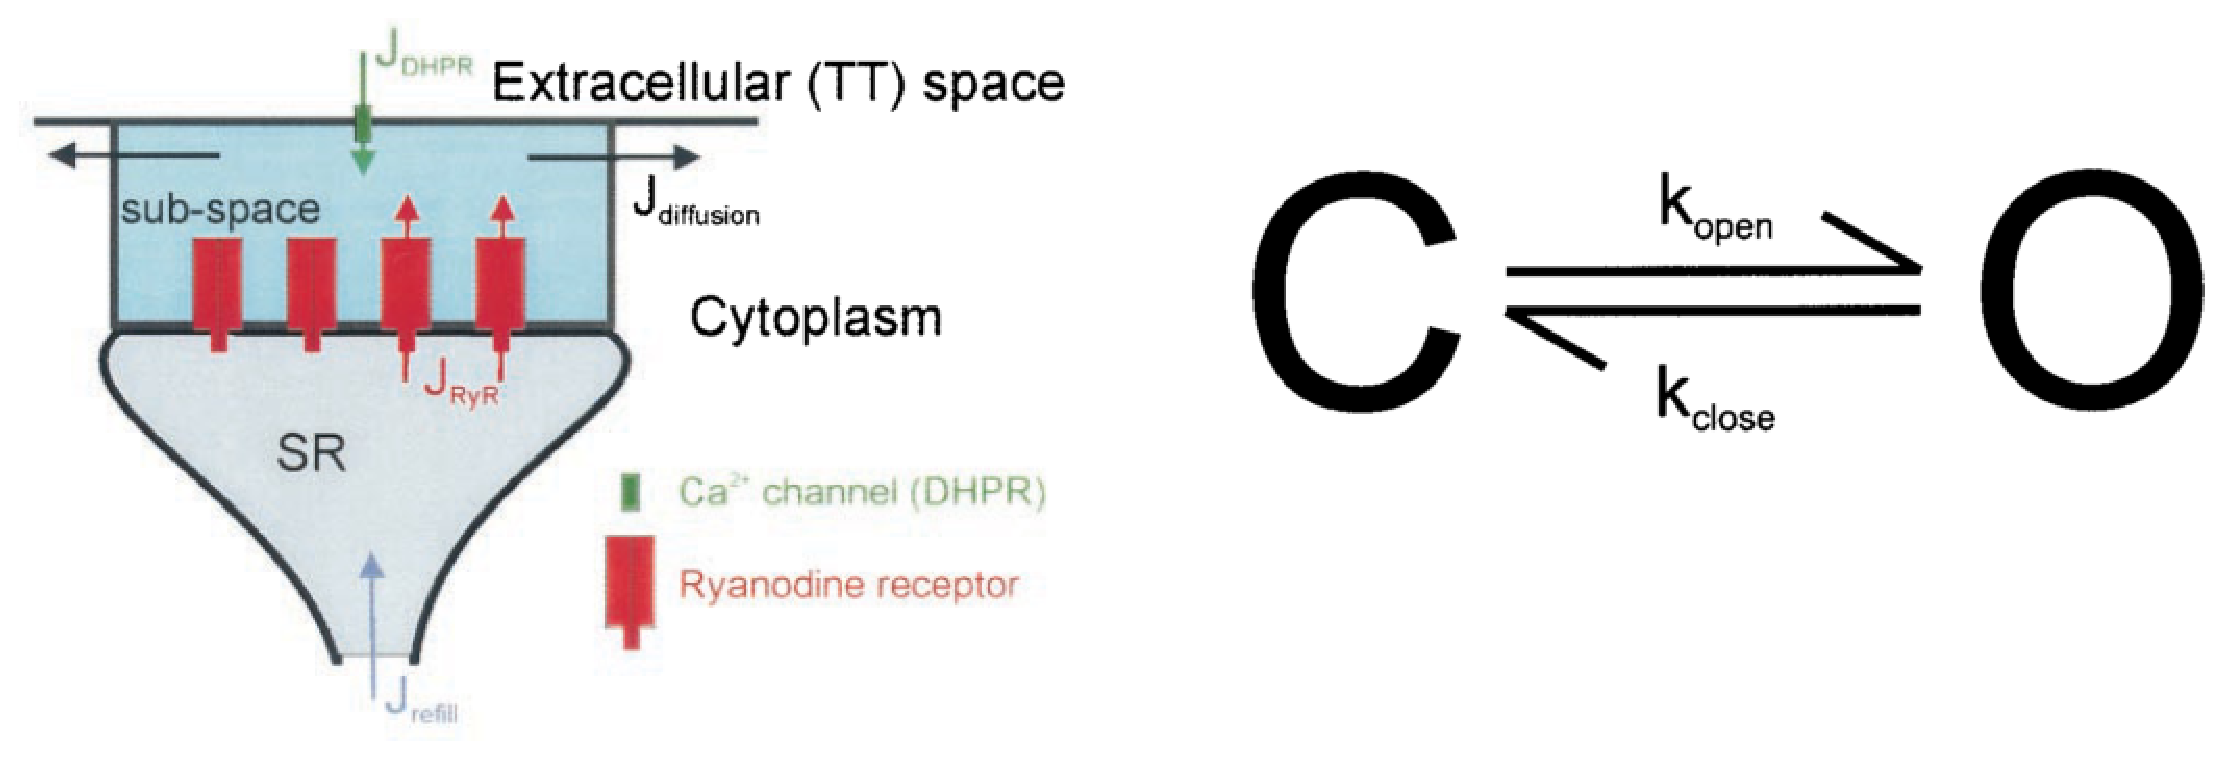
\includegraphics[height=3cm,
    angle=0]{./images/Sobie_Jafri-2002.eps}}
  \caption{Schematic diagram for the model of a subspace: a single DHPR
    + a cluster of RyRs. The arrows show the fluxes of calcium}
  \label{fig:Sobie_Jafri2002}
\end{figure}

Fig.~\ref{fig:Sobie_Jafri2002} shows the schematic diagram of a single
subspace being studied. The fluxes with the notations are standardized
as follows
\begin{enumerate}
\item $J_\text{release} = J_\ryr$ (rather than using $J_\ryr$ to refer
  to single RyR flux, and $J_\text{release}$ to refer to total RyR
  flux)
\item $J_\text{diffusion} = J_\ef$
\item $J_\dhpr$
\end{enumerate}

The spark model is similar to~\citep{smith1998}
(Sect.~\ref{sec:smith-et-al}), with 2 exceptions:
\begin{itemize}
\item SL buffers are confined to within the region 300nm of the CRU, the
concentration is linearly decreased with distance from the CRU
\item Fluo-3 $K_d=0.5\muM$ (rather than 1.13$\muM$). In order to make the time
course of the spark more closely resembled the experimentally observed data.
\end{itemize}

\subsection{Mathematical model}
\label{sec:mathematical-model-13}

In this model, bulk myoplasmic $\Ca$ and network SR $\Ca$ are assumed
to be constant. So, there are only two places where $\Ca$ changes
overtime: in the subspace and in the junctional SR.

\subsubsection{$[\Ca]_{ss}$}
\label{sec:calcium_subspace}

\begin{framed}
  The first important step is to define the reference volume for the
  flux. One way is to use the subspace volume e.g. $V_{ss}$ where
  contain the calcium concentration we first examine,
  e.g. $[\Ca]_{ss}$. Then, in the next parameters, e.g. $[\Ca]_{jsr}$,
  if we reuse these fluxes, we will map them to the corresponding
  volume by multiplying $V_{ss}/V_\text{jsr}$.

  In the destination volume is assumed to be much larger than the
  source volume, we can ignore that. 
\end{framed}

The dynamics of $[\Ca]_{ss}$ in a single subspace is given by the ODE
\begin{eqnarray}
  \label{eq:950}
  \frac{d[\Ca]_{ss}}{dt} = J_\ryr + J_\dhpr - J_\ef - J_\buf
\end{eqnarray}
with the individual fluxes are
\begin{eqnarray}
  \label{eq:951}
  J_\dhpr &&= \left\{
    \begin{array}{lc}
      0 &  (\text{ if DHPR closes})  \\
      \frac{\overline{I_{dhpr}}}{z_\ca F V_{ss}}   & (\text{if DHPR opens})
    \end{array}
  \right. \\
  J_\ryr &&=  N_\ryr^\circ v_\ryr ([\Ca]_{jsr} - [\Ca]_{ss}) \\
  J_\ef &&=  \frac{[\Ca]_{ss}-[\Ca]_\myo}{\tau_\ef} \\
  J_\buf &&= \sum_{i=\text{CaM,SR,SL}} k^i_{on} [\Ca]_{ss}[B_i] -
  k^i_{off}([B_i]_{tot} - [B]_i)
\end{eqnarray}
with
\begin{itemize}
\item $z_\ca=2$ the valence, F is Faraday constant and $\overline{I_\dhpr}
  = -0.5$(pA) is the single channel current.

\item $v_\ryr = 4000 (s^{-1})$ (or $D_\ryr$ in the original paper) is
  the rate of $\Ca$ through a single open RyR channel, and
  $N_\ryr^\circ$ is the number of RyR open.

\item $[\Ca]_\myo$ being held at a constant value. 

\item $[B_i]$ is the unbound buffer concentration, $[B_i]_{tot}$ is
  the total buffer concentration (bound+unbound) of buffer i which can
  be either calmodulin (CaM), buffer in SR or SL
\end{itemize}

% \begin{framed}
%   The time constants $\tau$ were chosen roughly equivalent to diffusion over
%   8-13nm (in myoplasm), and 0.5-1.58$\mu$m (in NSR), depending on the
%   true or effective diffusion constant for $\Ca$ is assumed. 
% \end{framed}

The geometry parameters of a single subspace are given in
Table~\ref{tab:Geometry_param}. The time constants $\tau$ is selected based on
their different characteristic distances, with are roughly equivalent to the diffusion
over a spatial scale of, 8-13nm and (in the myoplasm) 0.5-1.58$\mum$ (in the
NSR) (depending on whether the true or effective diffusion constant for
$\Ca$ is assumed). NOTE: $\tau=\frac{2.D}{x^2}$.

\begin{table}[hbt]
  \begin{center}
    \caption{Geometry parameters}
    \begin{tabular}{ccc} 
      \hline
      Symbol & Definition & Value \\ 
      \hline\hline
      $V_{ss}, V_{ds}$ & dyadic (diadic) subspace Volume & $10^{-13}\mu$L \\
      $V_{jsr}$ & junctional SR Volume & $10^{-11}\mu$L \\
      $\tau_\ef$ & efflux time constant & $7\times 10^{-7}$ s \\
      $\tau_\rf$ & efflux time constant & $0.01$ s \\
      $[\Ca]_\myo$ & bulk myoplasmic $\Ca$ concentration & $0.1\muM$ \\
      $[\Ca]_\nsr$ & network SR $\Ca$ concentration & $10^3\muM$ \\
    \end{tabular}
  \end{center}
  \label{tab:Geometry_param}
\end{table}

\subsubsection{$[\Ca]_{jsr}$}
\label{sec:calcium_jsr}

\begin{framed}
  The fluxes discussed in the previous section is reference to
  $V_{ss}$. In order to build a proper balanced system, all fluxes
  need to reference to the same volume. So, here, we need to map the
  fluxes to $V_{ss}$, by multiplying the flux terms with an adjusting
  coefficient $V_{ss}/V_\text{jsr}$
\end{framed}

The dynamics of $[\Ca]_{jsr}$ in a single calcium release unit is
given by the ODE
\begin{equation}
  \label{eq:953}
  \frac{d[\Ca]_{jsr}}{dt} = \beta_\jsr (J_\rf \frac{V_{ss}}{V_{jsr}} - J_\ryr )
\end{equation}
with
\textcolor{red}{ buffering in the JSR is assumed to be Casequestrin
  only}, with rapid approximation assumption~\citep{keizer1996rra}.
\begin{equation}
  \label{eq:956}
  \beta_\jsr = \frac{1}{1+\frac{[CSQ]_{tot}K_{CSQ}}{([CSQ]_{tot}+K_{CSQ})^2}}
\end{equation}
and
\begin{eqnarray}
  \label{eq:955}
  J_\rf = \frac{-[\Ca]_{jsr} + [\Ca]_{nsr}}{\tau_\rf}
\end{eqnarray}
with
\begin{itemize}
\item $[\Ca]_\nsr$ being held at a constant value. 
\end{itemize}


\subsubsection{RyR gating}
\label{sec:ryr-gating}


\begin{eqnarray}
  \label{eq:961}
  CF_{open} &&= 1 + \frac{N_{open}+ 1}{N_{open} + N_{close}} \\
  CF_{close} &&= k_{coop} \left( 1 + \frac{N_{close}+ 1}{N_{open} +
      N_{close}}  \right)
\end{eqnarray}
the scaling factor $k_{coop}$ was introduced to simulate the changes
in the strength of the coupling between RyRs. However, in control
condition, $k_{coop} = 1$.

It's also shown that, with a minimal model of RyR, a stable spark
termination can also be reproduced.
\begin{equation}
  \label{eq:958}
  \ce{C <=>[k_{open}][k_{close}] O}
\end{equation}
with
\begin{eqnarray}
  \label{eq:959}
  k_{close} &&= CF_{close} \times 480 \;\;\; (s^{-1}) \\
  k_{open} &&= CF_{open} \times 3 \times 10^4
  \frac{[\Ca]^4_{ss}}{[\Ca]^4_{ss} + K_m^4}  \;\;\; (s^{-1})
\end{eqnarray}
with RyR opening is favoured when luminal $[\Ca]$ is high, and it
follows a linear relationship
\begin{eqnarray}
  \label{eq:960}
  K_m = 6.0 - 0.0024 [\Ca]_{jsr} \;\;\; (\mu M)
\end{eqnarray}


\subsection{Numerical solution}
\label{sec:numerical-solutioin}

The behaviors of the model with the number of RyRs in a cluster ranging from 10
to 100 are studied using Monte Carlo method~\citep{rice1999mgg}.
A semi-implicit algoithm was used to solve in space and time, such that
diffusion of $[\Ca]$ and $[\CaF]$ were treated using Crank-Nicolson algorithm
(Sect.\ref{sec:Crank-Nicolson-method}),
while calcium buffering was treated explicitly. The model was implemented in
MatLab with time step $2\mus$. Results were produced using IDL, Origin and
CorelDraw softwares.

% At each time step, the system was solved using Euler's method with
% time step $dt = 10^{-8}$ (sec) or $10$(ns). The code was implemented
% in FORTRAN on an HP Visualize unix workstation.

The spark is triggered by opening the megachannel LCC $i_\dhpr=0.5$(pA) for
0.5ms, with $>98\%$ fidelity of spark triggering.


\subsection{Analysis}
\label{sec:analysis-13}

% Thus, in the
% simulation, we can simulate the influx of $\Ca$ from DHPR by
% triggering a stereotypical DHPR opening (0.5pA during 0.5ms), and it
% could trigger the spark with 98\% fidelity. 

The model is robust in the sense that $\ca$ spark duration and amplitude are
largely insensitive to the number of RyRs in a cluster. $P_o$ remains high
(close to 1) for 10ms, then quickly declines to zero after 25ms (Fig.2). The
re-opening is prevented because of the envolvement of $[\Ca]_\jsr$ in the
relationship between $P_o$ and $[\Ca]_\ds$.

Single channel activity cannot be detected using current imaging technology, due
to noise. This may explain the absence or near invisibility of $\Ca$ sparks in
cell systems with few or extremely small RyR clusters \citep{haak2001}.

The role of lumenal $\Ca$ is rigid. However, the mechanism is unknown, e.g.
free lumenal $\Ca$ regulate directly, or through $\Ca$ binding to an associated
protein such as Calsequestrin. This model assume the direct affect of free
lumenal $\Ca$.

\citep{sobie2006} suggested that weak coupling ($E_j$) between RyRs in the
cluster may facility the spark-induced-spark phenomena to occur, when they put
release sites of 50RyRs at 0.5$\mum$ in distance.
	
\section{Inoue-Bridge (2003) (rabbit)}
\label{sec:spark_Inoue-Bridge_2003}

Using 50 stimulus, and then capture 50 images, within 40ms after each stimulus.
By averaging F/F0 at the same location. NOTE: F/F0 $< 2$ in their data. The FWHM
of the $\Ca$ spark is 1.8$\mu$m. From experiments, FWHM in rat and mice is
2.0$\mu$m and 1.8$\mu$m. 

Line-scan image is captured every 2ms. So time to peak is 6-8 (ms),
corresponding to 3-4 pixels. The delay from the AP peak to the activation of the
sparks was from 2-6 (ms).

\begin{figure}[hbt]
  \centerline{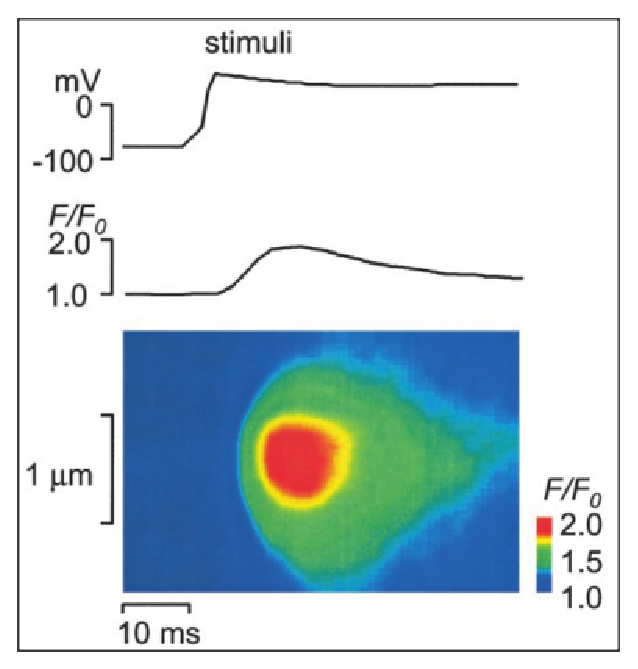
\includegraphics[height=5cm,
    angle=0]{./images/spark_Inoue2003.eps}}
\caption{Averaged signal: (A) AP, (B) F/F0, (C) line-scan image}
\label{fig:Wenckebach}
\end{figure}

Many experiments use +0 (mV) to study LCC behavior. However, to reach AP peak,
we need more positive potential, e.g. +50 (mV). At this positive potential, the
dynamics of LCC can be different. So, that's why some model use adaptive
formula, rather than a single equation.


\section{Hinch (2004)}
\label{sec:hinch-2004}

~\citep{hinch2004mag} conducted a mathematical analysis on spark frequencies,
spark duration distribution, using {\bf asymptotic analysis}. This is the single
CRU model with
\begin{enumerate}
  \item Bulk cytoplasm, dyadic subspace (height 10nm, width
  200nm, giving the volume 1.26$\times 10^{-3}\mum^3$)
  \citep{frank1990}, jSR and nSR.
  \item A cluster of RyRs, gating stochastically (coupled together and
  sensitive to jSR $\Ca$)
  \item $\Ca$ buffer in the dyadic subspace and jSR (Calmodulin and
  Calsequestrin)
\end{enumerate}

Two macro-states are built: one when the most RyRs are closed, and one when the
most RyRs are open. Asymptotic analysis is used to calculate the rate of
transitions between the two macroscopic states. The distribution of spark
lengths are analyzed using {\bf stochastic phase-plane analysis}
\citep{hinch2002prop}. 

The buffer in the subspace is calmodulin. It's assumed that the total
buffer concentration in the subspace is conversved, i.e. no diffusion of buffer
out of the subspace. Given the buffering time constant $\tau_B$, the dynamics of
the buffer is
\begin{equation}
\frac{d[\B]_\ds}{dt} = \frac{1}{\tau_B} \left( [\BCa]_\ds -
\frac{[\Ca]_\ds[\B]_\ds}{K_{d,\B}} \right)
\end{equation}
with $K_{d,\B}$ is the dissociation constant.

The dynamic equation of calcium in the subspace
\begin{equation}
V_\ds \frac{[\Ca]_\ds}{dt} = J_\ryr - J_\ef + \frac{V_\ds}{\tau_B}\left(
[\BCa]_\ds - \frac{[\Ca]_\ds[\B]_\ds}{K_{d,\B}} \right)
\end{equation}
with 
\begin{equation}
J_\ef = v_\ef ([\Ca]_\ds - [\Ca]_\myo)
\end{equation}
with $v_\ef$ is the rate of diffusion from the dyadic subspace. This value can
be approximated by considering (1) an area of interface between the subspace and
the bulk myoplasm, (2) the diffusion coefficient for $\Ca$, and (3) an effective
diffusion length. 





\section{Koh-\ldots-Levchenko (2006)}
\label{sec:koh_levchenko_2006}

\citep{koh2006} introduced a spatial model for a single release site to study
spark properties using stochastic simulation in 3D,
Fig.\ref{fig:dyad_space_Koh2006}. The stochastic nature of a few $\Ca$ ions in
the cleft space was modeled using random walks.


To study the variability of cleft geometry,they change $L_\text{cleft}$ from 100
to 500nm; yet the channel density remains unchanged, i.e. the wider the cleft,
the more channels in the release site.
Also, they study the change in coupling by varying $D_\text{cleft}$ distance;
here the number of channels doesn't change.
The role (1) of geometry (by varying $L_\text{cleft}$ and $D_\text{cleft}$), (2)
protein kinase (PKA)-mediated phosphorylation in $\Ca$ regulation in cleft were
examined.

\begin{figure}[hbt]
  \centerline{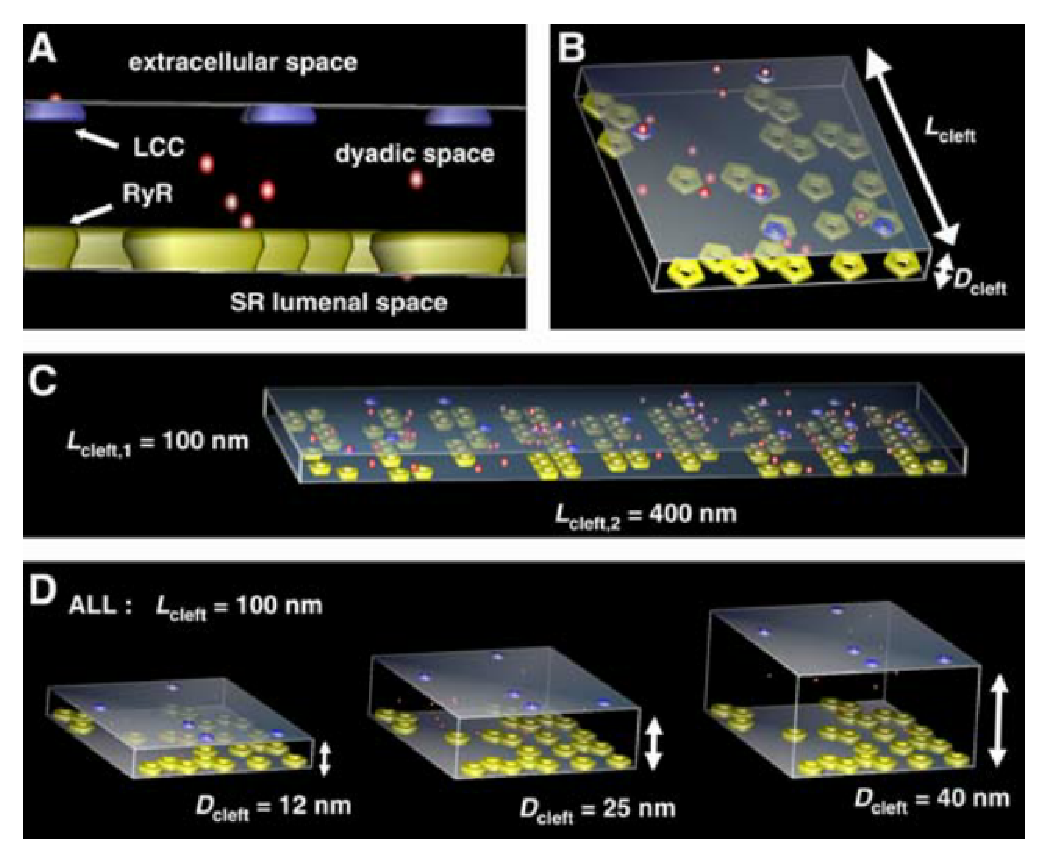
\includegraphics[height=4cm,
    angle=0]{./images/dyad_space_Koh2006.eps}}
\caption{The cleft model is assumed to be a rectangular space where the
distance betwen T-tubule and jSR membrane $D_\text{cleft}=12$nm. The lateral
section is square, each size is $L_\text{cleft,i}$ with $i=1,2,3$. (C)
$L_\text{cleft,1}=100nm, L_\text{cleft,2}=400nm$. (D) Models with variations in
$D_\text{cleft}$}
\label{fig:dyad_space_Koh2006}
\end{figure}

The volume of the cleft, i.e. dyadic subspace volume $V_\ds$, is estimated about
1.0-20.0$\times 10^{-13} \muL$ (if a cylindrical cleft is assumed). During $\Ca$
spark formation, the local $[\Ca]_\ds$ in this small compartment can reach a
peak of 100$\muM$ to 1mM during the first 10ms, and decline rapidly with a
half-time of 20ms, to the diastolic level of calcium ($\le 0.1\muM$). This
concentration of calcium translates to 1-2 calcium ions at rest, and $\sim 1000$
ions at peak.

\begin{framed}
The simulation is done by using MCell \url{http://www.mcell.cnl.salk.edu/}. This
tools allows tracking the position of individual molecules in space and time, as
well as predict how the change in physical environment might influence $\Ca$
signalling. 
\end{framed}




\subsection{Modelling}

The model for LCC is described in Sect.\ref{sec:LCC_Koh2006}. After 2 calcium
binding events, the channel enter the $\Ca$-inactivates state, with
high-affinity CaM sites. The recovery from this state is governed by
dissociation of $\Ca$ from the CaM/LCC complex. The model for RyR2 is based on
Sect.\ref{sec:RYR_Saftenku2001} with 8 states (5 closed, 3 open) in regular
setting; one state in $\Ca$-depedent inactivation (jumping from state O1 or C3).
The effect of RyR2 phosphorylation is incorporated with an additional state of
$\Ca$-dependent inactivation of this phosphorylated state.
The parameters on gating kinetics of phosphorylates states for the RyR2 model
are based on \citep{uehara2002}.

MCell software maps the positions of surfaces and effector sites in space, and
track the positions of individual diffusion molecules at every time steps. When
a ligand is detected at a point of intersection with a surface, there can be
different possible outcomes, depending on the current state of the
surfaces (e.g. reflective, transparent, absorptive, or occupied by an effector
site with an associated chemical reaction mechanism).

{\bf Boundary condition}: The four sidewalls of the dyadic subspace are modified
to absorb $\Ca$ when it comes to the border. The top and bottom surface of the
dyadic subspace is modeled to reflect $\Ca$ back into the cleft (jSR) or the
T-tubule, respectively. However, to avoid discontinuity in the diffusion
gradient along the edges of the cleft, larger volumes were placed around the
cleft, which moves the absorptive surfaces away from the boundaries of the cleft
and allowed reentry of $\Ca$ into the cleft. This pericleft volume didn't affect
significantly to the characteristics of the original $\Ca$ response (proved
in the paper). 

{\bf T-Tubule morphology disruption}: This was modelled by increasing the
distance between T-tubular wall and jSR wall, i.e. 20-50nm increase
\citep{lohn2000}. So, they studied it by varying $D_\text{cleft}$ from small
(9nm) to large (40nm). 

{\bf Densities of LCC and RyR2s}: A hypothetical dyadic cleft with 5 LCCs and 25
RyR2s. 

Unitary currents of RyR $\sim 0.1$ pA was used in the simulation. 

\subsection{Simulation method}

Based on Monte-Carlo simulation, at each time step only one reaction event (e.g.
single ion entry and single channel gating) is allowed to occur. The generation
of calcium is represented by channel in the open state transit to itself in the
next time step (indicated by {\it asterisks}). To simulate unitary current with
a reasonable accuracy, a time step should be small enough. Example: a single
channel current of 1.3pA is equivalent to the entry of 4 divalent ions per
$\mus$, or one ion per 0.25$\mus$. So, the time step should be smaller or equal
to 0.25$\mus$ to simulate any current not exceeding 1.3pA. 

The tool MCell was used \footnote{\url{www.mcell.cnl.salk.edu}}. MCell used
pseudo-random numbers to describe 3D Brownian random-walk for
diffusion and chemical reaction kinetics in complex spatial environments.
Reaction transaction probabilities are calculated according to user-specified
rate constants, then the probabilities are compared to the single random number
to determine which reaction to occur.

MCell allows user to define the model using a special model description
language, which MCell used to parse and create corresponding C++ objects and
simulation according to user instructions.
\begin{enumerate}
  \item geometry of the subcellular ultrastructure
  \item diffusion constant of diffusing ligands
  \item position of effector sites that interact with ligands
  \item chemical reaction mechanisms and kinetic rates constants governing the
  system
  \item appropriate time step and number of Monte Carlo time steps or iterations
  to simulate
\end{enumerate}

Simulations were done on dual Intel Xeon 1.0GHz workstation (Hummingbird Exceed
8.0 X-server). 100ms of physiological time took $\sim 3$min of computer time. 

\section{Higgins-\ldots-Sneyd (2006)}

\citep{higgins2007} used the software COMSOL Multiphysics to solve the finite
element method.

\section{Groff-Smith (2008)}
\label{sec:groff_smith_2008}

The dynamics of $\Ca$ sparks may arise due to the cooperative activity of RyRs
mediated by $\Ca$. In essence, individual channels are globally coupled via a
time-depenent or time-independent representation of the subspace $\Ca$, and
locally coupled with 2-4 neighboring channels. 

Modeling allosteric coupling is important in producing stable EC coupling. To
model this, \citep{stern1999lcm} use free energies of interactions between
neighboring channels. 

Similar to Sobie et al. method, mean-field approach is used; yet the ad-hoc term
is replaced by one derivied from the microscopic parameters of the $\Ca$ release
site. 

There are two things we need to investigate here: (1) the effect of
calcium coupling, (2) the effect of allosteric coupling between
neighboring RyRs. 

\textcolor{red}{\bf Calcium coupling}

Consider the cluster of $N$ RyRs in a planar ($z_n=0$), and we assume
linear superposing local $[\Ca]$ increase due to the contribution of
calcium diffusing from individual (opening) RyR channels at the
release site. So, the position of the RyR $n$-th can be written as
$\mathbf{r}_n=x_n.i+y_n.j$ (as $z_n=0$). Another assumption is the single (high
concentration) $\Ca$ buffer and the buffer is mobile. Then, based on
eq.\ref{eq:dCa}, the calcium concentration at an arbitrary point of coordinate
$\mathbf{r}=x.i+y.j+z.k$ is the summation of contribution from all channels
\begin{equation}
  \label{eq:1144}
  c(\mathbf{r})=\sum^N_{i=1}\frac{\sigma_n}{2\pi|\mathbf{r}_n-\mathbf{r}|(D_c+\kappa_\infty
    D_b)}\left[1+\frac{D_c + \kappa_\infty
    D_b}{D_c}\exp\frac{-|\mathbf{r}_n-\mathbf{r}|}{\lambda}\right]
\end{equation}
(NOTE: there's a typo in the original paper) with 
\begin{eqnarray}
  \label{eq:1145}
  \frac{1}{\tau} &&= k^+_bc_\infty + k^-_b \\
  \frac{1}{\lambda^2}&&=\frac{1}{\tau}\left(\frac{1}{D_b}+\frac{\kappa_\infty}{D_c}\right)
  \\
  \kappa_\infty &&= \frac{K_b[B]_T}{(K_b+c_\infty)^2} 
\end{eqnarray}
$\sigma_n=i_\ca/(2F)$ (when channel opens) or $\sigma_n=0$ (when channel closes)
is the source amplitude (i.e. number of $\Ca$ ions passing through per unit of
time) of the channel $n$. $D_c,D_b$ is diffusion  coefficient of free $\Ca$ and
buffer, respectively. $k^+_b,k^-_b$ is  the association/dissociation constant of
calcium binding. The  buffer is assumed rapid-buffering.

\begin{framed}
  The single mobile buffer is assumed Calmodulin-like buffer, i.e.
  $k^+_b=100\mu$M$^{-\eta}$.s$^{-1}$, $k^-_b=38$s$^{-1}$,
  $D_c=250\difu$, $D_b=32\difu$
\end{framed}
\begin{framed}
  There are different factors that may affect unitary RyR current,
  e.g. lumenal calcium.~\citep{groff2008} didn't include localized
  depletion of lumenal calcium, a phenomenon that is expected to
  reduce the effective unitary current of RyR {\it in vivo}. So, they
  assumed there are only 2 conducting states, and they are all the
  same for all channels
  \begin{equation}
    \label{eq:1132}
    \sigma_n(t) = \left\{
      \begin{array}{ll}
        0 & \text{if channel open}\\
        \overline{\sigma} & \text{if channel close}
      \end{array}
    \right.
  \end{equation}
  and all channels are assumed to have the same unitary current
  \begin{equation}
    \label{eq:1133}
    \overline{\sigma} = \frac{i_\ryr}{z_\ca F}
  \end{equation}
  $i_\ryr=0.4$pA.
\end{framed}

Typically, we want to know the concentration of calcium near the $\Ca$
regulatory site of the channel. Suppose the location of the regulatory site is
at a distance $r_d$ to the pore of the channel $m$ which is on the planar plane,
then the location of the regulatory site is $\mathbf{a}_m=x_m.i+y_m.j+r_d.k$,
and the calcium elevation at that position contributed by channel $n$ is
\begin{equation}
  \label{eq:1147}
  c_{nm}=\frac{\sigma_\circ}{2\pi|\mathbf{r}_n-\mathbf{a}_m|(D_c+\kappa_\infty
    D_b)}\left[1+\frac{D_c+ \kappa_\infty
    D_b}{D_c}\exp\frac{-|\mathbf{r}_n-\mathbf{a}_m|}{\lambda}\right]
\end{equation}
with $\sigma_n(t)=\sigma_\circ$ if the channel open.

Here, we assume linear summation of $\Ca$ concentration. So, the total calcium
at the regulatory site of channel $m$ at state $i$ is
\begin{equation}
  \label{eq:1148}
  c_{m(i)} = c_\infty + \sum^N_{n=1} \overline{c}_{nm_i}
\end{equation}
which is the calcium that involves in the determination of state change
of RyR $m$-th as depicted in eq.~\eqref{eq:1131}. Here
\begin{equation}
\overline{c}_{nm} = \left\{ \begin{array}{ll}
c_{nm} & \text{if $i_n$ is open} \\
0 & \text{otherwise}
\end{array}
\right.
\end{equation}

So, to consider the rate of $\Ca$-mediated transition for a single channel
$m$ from $i$ to $j$, we need to find $c_{m(j)}$ for all $j$.

In practice, the location of the calcium regulatory site is unknown, i.e. $r_d$
is unknown. The cryon-electron microscopy data suggest that RyR oligomer has a
large 29x29x12 nm cytoplasmic assembly. So, they choose $r_d = 30$ (nm). 

\begin{framed}
  The calcium coupling strength $c_{nm}$ can be adjusted by (1)
  changing the channel source amplitude, (2) buffer parameters, or (3)
  the diffusion constant for free $\Ca$.
\end{framed}

In situation, when they ignore the invidiual channels, i.e. mean-field
approach, we only consider how many channels in a given state. The coupling
strength is now defined as the average of off-diagonal elements in the coupling matrix
$\mathbf{C}=(c_{mn})$.
\begin{equation}
  \label{eq:1149}
  c^* = \frac{1}{N(N-1)}\sum^N_{
    \begin{array}{l}
      n,m=1\\
      n\ne m
    \end{array}
  }
  c_{nm}
\end{equation}
which is a decreasing function of $[\BT]$ for any fixed unitary
current $i_\ryr$, and increasing function of $i_\ryr$ for fixed
$[\BT]$, Fig. 2(C) in \citep{groff2008}. 

So, in the mean-field approach, to be discussed later, each opening
channel is assumed to contribute $c^*$ to the calcium elevation of
every other channel, then all channels in the cluster experience the
same calcium level
\begin{equation}
  \label{eq:1154}
  c_m = c_\infty + nc^*
\end{equation}

\textcolor{red}{\bf Allosteric coupling}

When two channels interact to each other, each one may create an allosteric
interaction on to another. To quantify such effect, a dimensionless
free energy term $\varepsilon_{ij}$ (in units of $k_BT$) is used. 
NOTE: As $E_{ij}$ and $k_BT$ has the same unit and $k_BT$ is the smallest energy
discretization, instead of using free energy $E_{ij}$ as  described in
~\citep{stern1999lcm},~\citep{groff2008} defined  dimensionless free energy
$\varepsilon_{ij}$ of interactions (in unit  of $k_BT$). 
So, the original formula in eq.~\eqref{eq:1130} can be written as
\begin{equation}
  \label{eq:1139}
  K_{ij} = k_{ij} \exp\left(-\eta_{ij}\sum^4_{m=1}(\varepsilon_{js_m}-\varepsilon_{is_m})\right)
\end{equation}
with $s_m$ is the state of the $m$-th neighboring channel.

Traditionally, the transition rates $k_{ij}$ are rate constants and 
are constants. However, the transition rate can now change due to
$\Ca$-dependency, a new notation we use is $q_\ij$. Then, \textcolor{blue}{the
new quantity of rate transition is $Q_{ij}$,  rather than $K_{ij}$}.

\begin{equation}
  \label{eq:1151}
  Q_{ij} = q_{ij} \exp\left(-\eta_{ij}\sum^4_{m=1}(\varepsilon_{js_m}-\varepsilon_{is_m})\right)
\end{equation}


These unitless interaction energies are organized into a matrix
$\mathcal{E}_{M\times M}$ with $M$ is the number of single-channel
states and $\varepsilon_{ij}=\varepsilon_{ji}$ ($i\ne j$) to satisfy
the requirement of thermodynamics reversibility. For example: $M=2$
\begin{equation}
  \label{eq:1135}
  \mathcal{E}=\left(
    \begin{array}{ll}
      \varepsilon_{CC} & \varepsilon_{CO}\\
      \varepsilon_{OC} & \varepsilon_{OO} 
    \end{array}
\right)
\end{equation}
and
\begin{equation}
  \label{eq:1152}
  \begin{split}
    q_{CO} &= k^+ c^\eta\\
    q_{OC} &= k^-
  \end{split}
\end{equation}

To know which channel is in adjacent to another, we build adjacent matrix
$\mathbf{A}$. \textcolor{red}{For $N$ channels in the dyad}, the adjacent matrix
is defined as
\begin{equation}
  \label{eq:1136}
  A = (a_{mn}) = \left\{
      \begin{array}{lc}
        1 & \text{if 2 channels $m$ and $n$ are adjacent} \\
        0 & \text{otherwise} \\
      \end{array}\right.
\end{equation}
NOTE: $a_{nn}=0$, as a channel does not experience allosteric
interaction with itself. So, using matrix notation, a convenient way
to formulate eq.~\eqref{eq:1151} for the channel $n'$ from state $i$
to $j$ is
\begin{equation}
  \label{eq:1140}
  Q_\ij = q_\ij \exp\left(-\eta_\ij(\gamma_j-\gamma_i) \right)
\end{equation}
with the total allosteric coupling energy imposing on each state is
\begin{equation}
  \label{eq:1141}
  \begin{split}
    \gamma_i &= \sum^N_{k=1}a_{kn'}\varepsilon_{k_s i}\\
    \gamma_j &= \sum^N_{k=1}a_{kn'}\varepsilon_{k_s j}
  \end{split}
\end{equation}
with $k_s$ is the state of the RyR $k$.
\textcolor{red}{NOTE: This is the Q-matrix for a single channel. In a cluster
with $N$ channel, we need to have $N$ Q-matrix for all channels in the cluster}.

Similar to~\citep{stern1999lcm}, to consider allosteric coupling, this
transition rate is modified by a coupling factor $\chi_{ij}$ 
\begin{equation}
  \label{eq:1138}
  \tilde{q_{ij}} = q_{ij}\chi_{ij}
\end{equation}
Utilize eq.~\eqref{eq:1140}, we have
\begin{equation}
  \label{eq:1142}
  \begin{split}
    \tilde{q_\ij} &=q_\ij\exp\left(-\eta_\ij(\gamma_j-\gamma_i)
    \right)\\
    \tilde{q_\ji} &=q_\ji\exp\left(\eta_\ji(\gamma_j-\gamma_i)
    \right)\\
  \end{split}
\end{equation}
So, with $n_\ij=1-n_\ji$, then $1 = (n_\ij+n_\ji)$ and
\begin{equation}
  \label{eq:1143}
  \frac{\tilde{q_\ij}}{\tilde{q_\ji}} = \frac{q_\ij}{q_\ji}\exp(-(\gamma_j-\gamma_i))
\end{equation}
\begin{framed}
  
  In general, $\eta_\ij$ can potentially receive different values for
  every transition $i$ to $j$. However, if we assume the transition
  rate involving the association of $\Ca$ are diffusion-limited,
  $\eta=0$ when channel makes transition from C to O, i.e. the change
  in free energy cannot increase the on-rate. Conversely, $\eta=1$ for
  all other configuration where channels make O to C transition.  So,
  for the 2-state RyR model:
  \begin{equation}
    \label{eq:1156}
    \begin{split}
      \tilde{q}_{CO} &= k^+c^\eta \\
      \tilde{q}_{OC} &= k^-\exp(-(\gamma_2-\gamma_1))
    \end{split}
  \end{equation}
\end{framed}

In the 2-state RyR model, using the assumption of diffusion-limited,
the allosteric energy is the combination of
$(\varepsilon_{CC}-\varepsilon_{CO})$ and
$(\varepsilon_{OC}-\varepsilon_{OO})$.

In the 3-state RyR model, e.g. $S1<=>S2<=>S3$, using the assumption of
diffusion-limited, the allosteric energy is the combination of
$(\varepsilon_{S_1S_2}-\varepsilon_{S_1S_1})$,
$(\varepsilon_{S_1S_2}-\varepsilon_{S_2S_2})$,
$(\varepsilon_{S_1S_3}-\varepsilon_{S_1S_1})$,
$(\varepsilon_{S_1S_3}-\varepsilon_{S_3S_3})$,
... In other words, the problem is getting much more complicated if we
consider 3-state and above. 

To simplify that, without the loss of generality, we can fix
$\varepsilon_{CO}=\varepsilon_{OC}=0$ or any $\varepsilon_{S_iS_j}=0$
with $i\ne j$. It means we focus on the allosteric interaction that
promotes synchronous gating, or no state change ($\varepsilon_{CC}\le
0, \varepsilon_{OO}\le 0$).

The experimental result showed that allosteric interaction is not
required for channel to exhibit synchronous gating. Indeed, coupled
gating can be mediated entirely via buffered diffusion of local
calcium as long as coupled strength is sufficient,
e.g. $c^*=0.75\mu$M. In the 2-state RyR model, optimal $c^*$ is an
increasing function of the magnitude of $\varepsilon_{CC}$. Indeed,
sparks depend on $c^*, \varepsilon_{CC}, \varepsilon_{OO}$ in a
complicated manner. 

\textcolor{red}{\bf Mean-field approximation}

In different computational studies, it was demonstrated that
{\bf mean-field approach} (i.e. ignoring the spatial arrangement of
RyRs) to modeling RyR clusters often perform well. So, ignoring the
position of individual channels in the cluster, we can get rid of
examining maximum 4 neighbors for each channel. However, instead of
using the ad-hoc approach like ~\citep{sobie2002tcas}
(Sect.~\ref{sec:RYR_Sobie2002}),~\citep{groff2008} simplified Stern
{\it et al.} approach and solve it using matrix computational
approach.

So, when the locations are not important, all RyRs are
indistinguishable and the adjacent matrix can be now mapped to a new
form $\mathbf{\overline{A}}=(a^*)$, where $0\le a^*\le 1$ is the average
allosteric connectivity
\begin{equation}
  \label{eq:1150}
  a^* = \frac{1}{N(N-1)}\sum^N_{
    \begin{array}{l}
      n,m=1\\
      n\ne m
    \end{array}
  }
  a_{nm}
\end{equation}
Then, the calcium coupling contribute to each channel can be assumed
to be the same $\mathbf{\overline{C}} = (c^*)$

\begin{framed}
  NOTE: It's impossible to generate a cluster of RyR that satisfies
  any of the two assumptions: $c^*$ and $a^*$. However, it simplifies
  dramatically the computational demand and the simulation results are
  still reasonable.
\end{framed}

The old definition of a state of a cluster is
$\mathbf{i}=(s_1,s_2,...,s_N)$ in which $s_i$ is the current state of
channel $i$, $s_i=1..M$. Using mean-field approach, the new definition
of a state of a cluster is $\mathbf{i}=(n_1,n_2,...,n_M)$, with $n_i$
is the number of channels in the cluster in state $i$. So, if the next
state is $\mathbf{j}=(n_1-1,n_2+1,...,n_M)$, there are $n_1$ chances
for a channel to switch from state $\mathbf{i}$ to state $\mathbf{j}$,
i.e.
\begin{equation}
  \label{eq:1155}
  q_\ij = n_1 k^+ (c_\infty + N_O c^*)^\eta
\end{equation}
with $N_O$ is the number of open channel

Consider the 2-state RyR model above:
\begin{equation}
  \label{eq:1153}
  \begin{split}
    \tilde{q}_{CO} &= (N-N_O)k^+(c_\infty + N_O.c^*)^\eta\\
    \tilde{q}_{OC} &= k^- N_O
    \exp\left(-(a^*(N_O-1)(\varepsilon_{OC}-\varepsilon_{OO})-(N-N_O)
      a^*(\varepsilon_{CC}-\varepsilon_{CO}))\right)
  \end{split}
\end{equation}
Using the assumption of calcium diffusion-limited, we have
\begin{equation}
  \label{eq:1157}
  \tilde{q}_{OC} = k^- N_O
  \exp\left(-a^*(-(N_O-1)\varepsilon_{OO}-(N-N_O)
    \varepsilon_{CC})\right)  
\end{equation}


\section{Laver-\ldots-Cannell (2012)}
\label{sec:laver_cannell_2012}

\citep{laver2012} built a 3D model of the cardiac dyad for rat ventricular cell
at physiological condition. The termination was robust, i.e. insensitive to the
number of RyRs in the cluster and automatic. However, the model assumed that
intrinsic inactivation of the channels and lumenal calcium depletion is not
necessary for spark termination. Here, jSR is reduced to about 10\% of resting
level (i.e. $[\Ca]_\jsr=100\muM$) that reduced the calcium flux via RyR due
to the reduced gradient between Ca-jSR and Ca-dyad. In their model, the
threshold is about 70$\muM$. The RyR closed time has a steep calcium dependence,
i.e. the opening rate (per second) reduced significantly with reducing Ca-jSR.

They measure RyR opening and closing rates as a function of $[\Ca]$ based on
the setting that RyRs are incorporated into planar lipid bilayer in the presence
of $\Mg$ and ATP (See Sect.\ref{sec:RyR_Laver2012}). The geometry is
derived from electron micrographs.

The nSR and jSR contains the buffer calsequestrin (CSQ), distributed throughout
the space. Myplasmic buffers included troponin (Trpn), Calmodulin (CMD), Fluo-3,
ATP, as well as fixed binding sites on the T-tubules and SR membranes. The
cluster has 36 RyRs (triggered by influx of calcium via $I_\dhpr=0.2$ pA for
3ms). 

They modeled 
\begin{enumerate}
  \item T-tubule of diameter 250nm \citep{}
  \item The subspace with 26nm high
\citep{} and 360nm long and 450nm around the T-tubule circumferene
   \item The jSR has a diameter of 31nm
   \item The nSR occupied 3.5\% of the cytoplasmic volume \citep{}
   \item The center to center distance between RyRs was set to 31nm \citep{}
\end{enumerate}

The model encompass a volume of 50$\mum^3$ with reflective boundaries (i.e.
Von-Neumann with zero-flux were located at $\pm 2\mum$ in r and z).
The volume is divided into 18 slices along the x-axis of the tubule (z), 13
radial rings (r) and 16 segments around the axis ($\theta$) giving 3744 volume
elements. Polar coordinates were used to calculate the diffusion using Laplacian
\begin{equation}
\nabla^2 = \frac{\partial ^2}{\partial r^2} +
\frac{1}{r}\frac{\partial}{\partial r} +
\frac{1}{r^2}\frac{\partial^2}{\partial \theta^2} + \frac{\partial^2}{\partial
z^2}
\end{equation}
with finite difference method on a non-linear cylindrical grid. 


The flux is defined as
\begin{equation}
J_\ryr = \frac{K_\ryr}{V_\ds} \left( [\Ca]_\jsr - [\Ca]_\ds \right)
\end{equation}
with $K_\ryr$ is a constant so that single channel RyR is set to
$i_{1,\ryr}=0.6$ pA \citep{17,18} at $[\Ca]_\jsr = 1$ mM.

SERCA pump modeled was based on reverse-mode of Shannon et al. \citep{}
\textcolor{red}{which is not a realistic one}. 

\section{Hake et al. (2012)}

\section{(need to revise) $\Ca$ gradients in the neighboring of a channel}
\label{sec:calcium-gradient-neighborhood-channels}

For simplicity, we ignore calcium buffering, as most cytosolic buffers
are stationary and locate on myofilaments or other membranes or
organelles~\citep{stern1992tec}. Another assumption is that the
channel is treated as a point source at which $\Ca$ flux rate is $s$
(mol/s). 
\begin{enumerate}
\item The calcium concentration $C$ in the region around the channel
  pore is governed by
  \begin{equation}
    \label{eq:994}
    \frac{\partial C}{\partial t} = D\nabla^2C
  \end{equation}

\item assume the channel close at $t=0$ and then open for a some time
  which leads to the steady-state condition.  Then, the steady-state
  solution of eq.~\eqref{eq:994} is
  \begin{equation}
    \label{eq:995}
    C_\circ = \frac{s}{2\pi Dr} = \frac{s}{2\pi D\sqrt{(x^2+y^2+z^2)}}
  \end{equation}
  The factor 2 (rather than 4) in the denominator means that all calcium
  issuing from the channel pore goes to the cytosolic side, unlike true
  isotropic point source.
\item The concentration of free calcium at a distance $r$ from the
  pore, at time $t$ after the channel closure is
  \begin{equation}
    \label{eq:996}
    C = \frac{s.\erf\{\frac{r}{2\sqrt{Dt}}\}}{2\pi Dt}
  \end{equation}

  The result shows that there is a large local excess concentration of
  calcium above ambient cytosolic levels when the channel is open, and
  this excess dissipates within a fraction of a milliseconds after the
  channel closes. 

\end{enumerate}


%%% Local Variables: 
%%% mode: latex
%%% TeX-master: "mainfile"
%%% End: 
